\documentclass{amsart}
%\usepackage{morefloats}
\usepackage{tikz}
\usetikzlibrary{knots,intersections,decorations.pathreplacing,hobby}
 
\newcommand{\Braid}     {\operatorname{Braid}}

\newcommand{\N}         {\mathbb{N}}
\newcommand{\Z}         {\mathbb{Z}}
\newcommand{\R}         {\mathbb{R}}
\newcommand{\C}         {\mathbb{C}}

\newcommand{\al}        {\alpha}
\newcommand{\bt}        {\beta}
\newcommand{\ep}        {\epsilon}
\newcommand{\tht}       {\theta}

\newcommand{\Sg}        {\Sigma}

\newcommand{\ab}        {\overline{a}}
\newcommand{\bb}        {\overline{b}}
\newcommand{\cb}        {\overline{c}}
\newcommand{\db}        {\overline{d}}
\newcommand{\eb}        {\overline{e}}
\newcommand{\fb}        {\overline{f}}
\newcommand{\gb}        {\overline{g}}
\newcommand{\pb}        {\overline{p}}
\newcommand{\qb}        {\overline{q}}
\newcommand{\rb}        {\overline{r}}
\newcommand{\ub}        {\overline{u}}
\newcommand{\vb}        {\overline{v}}
\newcommand{\wb}        {\overline{w}}
\newcommand{\xb}        {\overline{x}}
\newcommand{\yb}        {\overline{y}}
\newcommand{\zb}        {\overline{z}}

\newcommand{\tu}        {\widetilde{u}}

\newcommand{\lk}        {\operatorname{lk}}
\newcommand{\ip}[1]     {\langle #1\rangle}
\newcommand{\un}[1]     {\langle\!\langle #1\rangle\!\rangle}
\newcommand{\st}        {\;|\;}
\newcommand{\tm}        {\times}
\newcommand{\ov}        {\overline}
\newcommand{\sse}       {\subseteq}
\newcommand{\sm}        {\setminus}

\renewcommand{\:}       {\colon}


\tikzset{every path/.style={blue,ultra thick}, every node/.style={transform shape, knot crossing, inner sep=2.5pt}}


\begin{document}

\tikzset{every path/.style={blue,very thick}, every node/.style={transform shape, knot crossing, inner sep=2.5pt}}

\begin{center}
 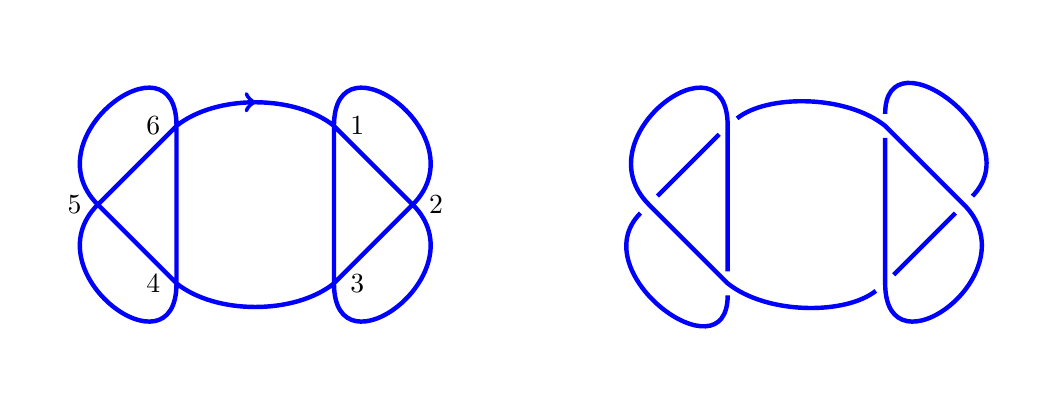
\begin{tikzpicture}
  \begin{scope}
   \begin{scope}
    \node (a) at (-1.0, 1) {};
    \node (b) at (-2, 0) {};
    \node (c) at (-1.0,-1) {};
    \node (d) at ( 1.0, 1) {};
    \node (e) at ( 2, 0) {};
    \node (f) at ( 1.0,-1) {};
    \draw (a.center) .. controls (-0.5,1.4) and (0.5,1.4) ..
          (d.center) .. controls (d.8 south east) and (e.8 north west) ..
          (e.center) .. controls (e.8 south east) and (f.8 south) ..
          (f.center) .. controls (f.8 north) and (d.8 south) ..
          (d.center) .. controls (d.8 north) and (e.8 north east) ..
          (e.center) .. controls (e.8 south west) and (f.8 north east) ..
          (f.center) .. controls (0.5,-1.4) and (-0.5,-1.4) ..
          (c.center) .. controls (c.8 north west) and (b.8 south east) ..
          (b.center) .. controls (b.8 north west) and (a.8 north) ..
          (a.center) .. controls (a.8 south) and (c.8 north) ..
          (c.center) .. controls (c.8 south) and (b.8 south west) ..
          (b.center) .. controls (b.8 north east) and (a.8 south west) ..
          (a.center) ;
    \draw[black] (d) node[anchor=west] {$1$};
    \draw[black] (e) node[anchor=west] {$2$};
    \draw[black] (f) node[anchor=west] {$3$};
    \draw[black] (c) node[anchor=east] {$4$};
    \draw[black] (b) node[anchor=east] {$5$};
    \draw[black] (a) node[anchor=east] {$6$};
    \draw[->] (0,1.3) -- +(0.01,0);
   \end{scope}
  \end{scope}
  \begin{scope}[xshift=7cm]
   \begin{scope}
    \node (a) at (-1.0, 1) {};
    \node (b) at (-2, 0) {};
    \node (c) at (-1.0,-1) {};
    \node (d) at ( 1.0, 1) {};
    \node (e) at ( 2, 0) {};
    \node (f) at ( 1.0,-1) {};
    \draw (a)        .. controls (-0.5,1.4) and (0.5,1.4) ..
          (d.center) .. controls (d.8 south east) and (e.8 north west) ..
          (e.center) .. controls (e.8 south east) and (f.8 south) ..
          (f.center) .. controls (f.8 north) and (d.8 south) ..
          (d)        .. controls (d.8 north) and (e.8 north east) ..
          (e)        .. controls (e.8 south west) and (f.8 north east) ..
          (f)        .. controls (0.5,-1.4) and (-0.5,-1.4) ..
          (c.center) .. controls (c.8 north west) and (b.8 south east) ..
          (b.center) .. controls (b.8 north west) and (a.8 north) ..
          (a.center) .. controls (a.8 south) and (c.8 north) ..
          (c)        .. controls (c.8 south) and (b.8 south west) ..
          (b)        .. controls (b.8 north east) and (a.8 south west) ..
          (a);
   \end{scope}
  \end{scope}
 \end{tikzpicture}
\end{center}


\begin{center}
 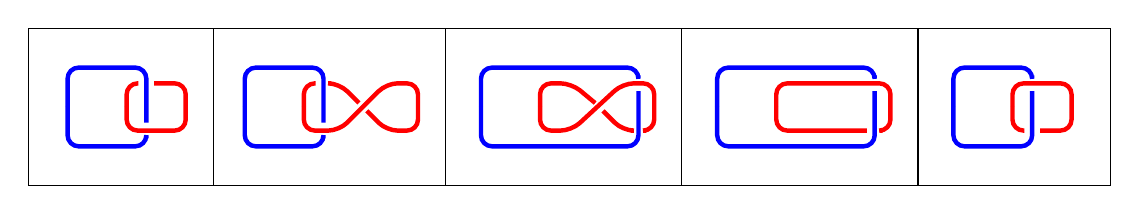
\begin{tikzpicture}[scale=0.5]
  \draw[thin,black] (-2,-2) rectangle (25.5,2);
  \draw[thin,black] (2.7,2) -- (2.7,-2);
  \draw[thin,black] ( 8.6,2) -- ( 8.6,-2);
  \draw[thin,black] (14.6,2) -- (14.6,-2);
  \draw[thin,black] (20.6,2) -- (20.6,-2);
  \begin{scope}
   \draw[rounded corners] (-1,0) -- (-1,1) -- (1,1) -- (1,-0.4);
   \draw[rounded corners] (1,-0.8) -- (1,-1) -- (-1,-1) -- (-1,0);
   \draw[red,rounded corners] (0.5,0) -- (0.5,-0.6) -- (2,-0.6) -- (2,0.6) -- (1.2,0.6);
   \draw[red,rounded corners] (0.8,0.6) -- (0.5,0.6) -- (0.5,0); 
  \end{scope}
  \begin{scope}[xshift=4.5cm]
   \draw[rounded corners] (-1,0) -- (-1,1) -- (1,1) -- (1,-0.4);
   \draw[rounded corners] (1,-0.8) -- (1,-1) -- (-1,-1) -- (-1,0);
   \draw[red,rounded corners]
     (0.5,0) -- (0.5,-0.6) -- (1.4,-0.6) -- (2.6,0.6) -- (3.4,0.6) --
     (3.4,-0.6) -- (2.6,-0.6) -- (2.1,-0.1);
   \draw[red,rounded corners]
     (1.9, 0.1) -- (1.4,0.6) -- (1.2,0.6);
   \draw[red,rounded corners] (0.8,0.6) -- (0.5,0.6) -- (0.5,0); 
  \end{scope}
  \begin{scope}[xshift=10.5cm]
   \draw[rounded corners] (-1,0) -- (-1,1) -- (3,1) -- (3,0.8);
   \draw[rounded corners] (3,0.4) -- (3,-1) -- (-1,-1) -- (-1,0);
   \draw[red,rounded corners]
    (0.5,0) -- (0.5,-0.6) -- (1.3,-0.6) -- (2.6,0.6) -- (3.4,0.6) --
    (3.4,-0.6) -- (3.2,-0.6);
   \draw[red,rounded corners]
    (2.8,-0.6) -- (2.6,-0.6) -- (2.1,-0.1);
   \draw[red,rounded corners]
    (1.9,0.1) -- (1.3,0.6) -- (0.5,0.6) -- (0.5,0); 
  \end{scope}
  \begin{scope}[xshift=16.5cm]
   \draw[rounded corners] (-1,0) -- (-1,1) -- (3,1) -- (3,0.8);
   \draw[rounded corners] (3,0.4) -- (3,-1) -- (-1,-1) -- (-1,0);
   \draw[red,rounded corners]
    (0.5,0) -- (0.5,-0.6) -- (2.8,-0.6);
   \draw[red,rounded corners]
    (3.2,-0.6) -- (3.4,-0.6) -- (3.4,0.6) -- (0.5,0.6) -- (0.5,0); 
  \end{scope}
  \begin{scope}[xshift=22.5cm]
   \draw[rounded corners] (-1,0) -- (-1,1) -- (1,1) -- (1,0.8);
   \draw[rounded corners] (1,0.4) -- (1,-1) -- (-1,-1) -- (-1,0);
   \draw[red,rounded corners]
    (0.5,0) -- (0.5,-0.6) -- (0.8,-0.6);
   \draw[red,rounded corners]
    (1.2,-0.6) -- (2,-0.6) -- (2,0.6) -- (0.5,0.6) -- (0.5,0); 
  \end{scope}
 \end{tikzpicture}
\end{center}



  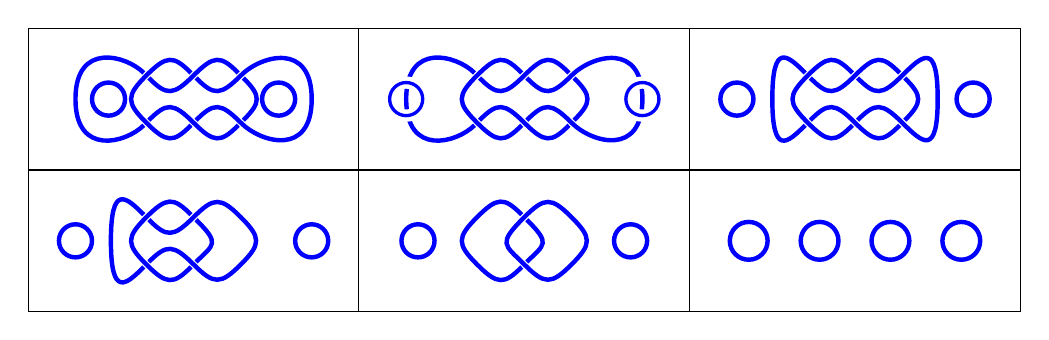
\begin{tikzpicture}[scale=0.3]
   \begin{scope}
    \node (p) at (-5, 0) {};
    \node (q) at ( 5, 0) {};
    \node (a) at (-2, 1) {};
    \node (b) at ( 0, 1) {};
    \node (c) at ( 2, 1) {};
    \node (d) at (-2,-1) {};
    \node (e) at ( 0,-1) {};
    \node (f) at ( 2,-1) {};
    \draw 
     (a)        .. controls (a.8 south east) and (b.8 south west) ..
     (b.center) .. controls (b.8 north east) and (c.8 north west) ..
     (c)        .. controls (c.8 south east) and (f.8 north east) ..
     (f)        .. controls (f.8 south west) and (e.8 south east) ..
     (e.center) .. controls (e.8 north west) and (d.8 north east) ..
     (d)        .. controls (d.8 south west) and (p.16 south) ..
     (p.center) .. controls (p.16 north) and (a.8 north west) ..
     (a);
    \draw 
     (c.center) .. controls (c.8 south west) and (b.8 south east) ..
     (b)        .. controls (b.8 north west) and (a.8 north east) ..
     (a.center) .. controls (a.8 south west) and (d.8 north west) ..
     (d.center) .. controls (d.8 south east) and (e.8 south west) ..
     (e)        .. controls (e.8 north east) and (f.8 north west) ..
     (f.center) .. controls (f.8 south east) and (q.16 south) ..
     (q.center) .. controls (q.16 north) and (c.8 north east) ..
     (c.center);
    \draw (-3.6,0) circle(0.7);
    \draw ( 3.6,0) circle(0.7);
    \draw[thin,black] (-7,-3) rectangle (7,3);
   \end{scope}
   \begin{scope}[xshift=14cm]
    \node (p) at (-5, 0) {};
    \node (q) at ( 5, 0) {};
    \node (a) at (-2, 1) {};
    \node (b) at ( 0, 1) {};
    \node (c) at ( 2, 1) {};
    \node (d) at (-2,-1) {};
    \node (e) at ( 0,-1) {};
    \node (f) at ( 2,-1) {};
    \draw 
     (a)        .. controls (a.8 south east) and (b.8 south west) ..
     (b.center) .. controls (b.8 north east) and (c.8 north west) ..
     (c)        .. controls (c.8 south east) and (f.8 north east) ..
     (f)        .. controls (f.8 south west) and (e.8 south east) ..
     (e.center) .. controls (e.8 north west) and (d.8 north east) ..
     (d)        .. controls (d.8 south west) and (p.16 south) ..
     (p.center) .. controls (p.16 north) and (a.8 north west) ..
     (a);
    \draw 
     (c.center) .. controls (c.8 south west) and (b.8 south east) ..
     (b)        .. controls (b.8 north west) and (a.8 north east) ..
     (a.center) .. controls (a.8 south west) and (d.8 north west) ..
     (d.center) .. controls (d.8 south east) and (e.8 south west) ..
     (e)        .. controls (e.8 north east) and (f.8 north west) ..
     (f.center) .. controls (f.8 south east) and (q.16 south) ..
     (q.center) .. controls (q.16 north) and (c.8 north east) ..
     (c.center);
    \draw[draw=white,double=blue ,ultra thick,double distance=1.2pt] (-5,0) circle(0.7);
    \draw[draw=white,double=blue ,ultra thick,double distance=1.2pt] ( 5,0) circle(0.7);
    \draw[thin,black] (-7,-3) rectangle (7,3);
   \end{scope}
   \begin{scope}[xshift=28cm]
    \node (p) at (-3.5, 0) {};
    \node (q) at ( 3.5, 0) {};
    \node (a) at (-2, 1) {};
    \node (b) at ( 0, 1) {};
    \node (c) at ( 2, 1) {};
    \node (d) at (-2,-1) {};
    \node (e) at ( 0,-1) {};
    \node (f) at ( 2,-1) {};
    \draw 
     (a)        .. controls (a.8 south east) and (b.8 south west) ..
     (b.center) .. controls (b.8 north east) and (c.8 north west) ..
     (c)        .. controls (c.8 south east) and (f.8 north east) ..
     (f)        .. controls (f.8 south west) and (e.8 south east) ..
     (e.center) .. controls (e.8 north west) and (d.8 north east) ..
     (d)        .. controls (d.8 south west) and (p.16 south) ..
     (p.center) .. controls (p.16 north) and (a.8 north west) ..
     (a);
    \draw 
     (c.center) .. controls (c.8 south west) and (b.8 south east) ..
     (b)        .. controls (b.8 north west) and (a.8 north east) ..
     (a.center) .. controls (a.8 south west) and (d.8 north west) ..
     (d.center) .. controls (d.8 south east) and (e.8 south west) ..
     (e)        .. controls (e.8 north east) and (f.8 north west) ..
     (f.center) .. controls (f.8 south east) and (q.16 south) ..
     (q.center) .. controls (q.16 north) and (c.8 north east) ..
     (c.center);
    \draw (-5,0) circle(0.7);
    \draw ( 5,0) circle(0.7);
    \draw[thin,black] (-7,-3) rectangle (7,3);
   \end{scope}
   \begin{scope}[yshift=-6cm]
    \node (p) at (-3.5, 0) {};
    \node (q) at ( 3.5, 0) {};
    \node (a) at (-2, 1) {};
    \node (b) at ( 0, 1) {};
    \node (c) at ( 2, 1) {};
    \node (d) at (-2,-1) {};
    \node (e) at ( 0,-1) {};
    \node (f) at ( 2,-1) {};
    \draw 
     (b.center) .. controls (b.8 north east) and (c.8 north west) ..
     (c.center) .. controls (c.8 south east) and (f.8 north east) ..
     (f.center) .. controls (f.8 south west) and (e.8 south east) ..
     (e.center) .. controls (e.8 north west) and (d.8 north east) ..
     (d)        .. controls (d.8 south west) and (p.16 south) ..
     (p.center) .. controls (p.16 north) and (a.8 north west) ..
     (a)        .. controls (a.8 south east) and (b.8 south west) ..
     (b.center);
    \draw 
     (b)        .. controls (b.8 north west) and (a.8 north east) ..
     (a.center) .. controls (a.8 south west) and (d.8 north west) ..
     (d.center) .. controls (d.8 south east) and (e.8 south west) ..
     (e)        .. controls (e.8 north east) and (f.8 north west) ..
     (b);
    \draw (-5,0) circle(0.7);
    \draw ( 5,0) circle(0.7);
    \draw[thin,black] (-7,-3) rectangle (7,3);
   \end{scope}
   \begin{scope}[yshift=-6cm,xshift=14cm]
    \node (p) at (-3.5, 0) {};
    \node (q) at ( 3.5, 0) {};
    \node (a) at (-2, 1) {};
    \node (b) at ( 0, 1) {};
    \node (c) at ( 2, 1) {};
    \node (d) at (-2,-1) {};
    \node (e) at ( 0,-1) {};
    \node (f) at ( 2,-1) {};
    \draw 
     (b.center) .. controls (b.8 north east) and (c.8 north west) ..
     (c.center) .. controls (c.8 south east) and (f.8 north east) ..
     (f.center) .. controls (f.8 south west) and (e.8 south east) ..
     (e.center) .. controls (e.8 north west) and (d.8 north east) ..
     (b.center);
    \draw 
     (b)        .. controls (b.8 north west) and (a.8 north east) ..
     (a.center) .. controls (a.8 south west) and (d.8 north west) ..
     (d.center) .. controls (d.8 south east) and (e.8 south west) ..
     (e)        .. controls (e.8 north east) and (f.8 north west) ..
     (b);
    \draw (-4.5,0) circle(0.7);
    \draw ( 4.5,0) circle(0.7);
    \draw[thin,black] (-7,-3) rectangle (7,3);
   \end{scope}
   \begin{scope}[yshift=-6cm,xshift=28cm]
    \draw[thin,black] (-7,-3) rectangle (7,3);
    \draw (-4.5,0) circle(0.8);
    \draw (-1.5,0) circle(0.8);
    \draw ( 1.5,0) circle(0.8);
    \draw ( 4.5,0) circle(0.8);
   \end{scope}
  \end{tikzpicture}

\begin{center}
 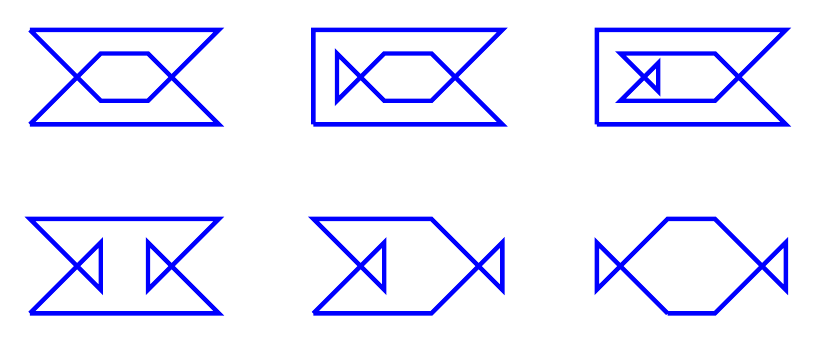
\begin{tikzpicture}[scale=0.6]
  \begin{scope}
   \draw (-2,-1) -- (2,-1) -- (0.5, 0.5) -- (-0.5, 0.5) -- (-2,-1);
   \draw (-2, 1) -- (2, 1) -- (0.5,-0.5) -- (-0.5,-0.5) -- (-2, 1);
  \end{scope}
  \begin{scope}[xshift=6cm]
   \draw (-2,-1) -- (2,-1) -- (0.5, 0.5) -- (-0.5, 0.5) -- (-1.5,-0.5) --
         (-1.5,0.5) -- (-0.5,-0.5) -- (0.5,-0.5) -- (2,1) -- (-2,1) -- (-2,-1);
  \end{scope}
  \begin{scope}[xshift=12cm]
   \draw (-2,-1) -- (2,-1) -- (0.5, 0.5) -- (-1.5, 0.5) -- (-0.7,-0.3) --
         (-0.7,0.3) -- (-1.5,-0.5) -- (0.5,-0.5) -- (2,1) -- (-2,1) -- (-2,-1);
  \end{scope}
  \begin{scope}[yshift=-4cm]
   \draw (-2,-1) -- (2,-1) -- (0.5,0.5) -- (0.5,-0.5) -- (2,1) --
         (-2,1) -- (-0.5,-0.5) -- (-0.5,0.5) -- (-2,-1);
  \end{scope}
  \begin{scope}[xshift=6cm,yshift=-4cm]
   \draw (-2,-1) -- (0.5,-1) -- (2,0.5) -- (2,-0.5) -- (0.5,1) -- 
         (-2,1) -- (-0.5,-0.5) -- (-0.5,0.5) -- (-2,-1);
  \end{scope}
  \begin{scope}[xshift=12cm,yshift=-4cm]
   \draw (-0.5,-1) -- (0.5,-1) -- (2,0.5) -- (2,-0.5) -- (0.5,1) -- 
         (-0.5,1) -- (-2,-0.5) -- (-2,0.5) -- (-0.5,-1);
  \end{scope}
 \end{tikzpicture}
\end{center}

\begin{center}
 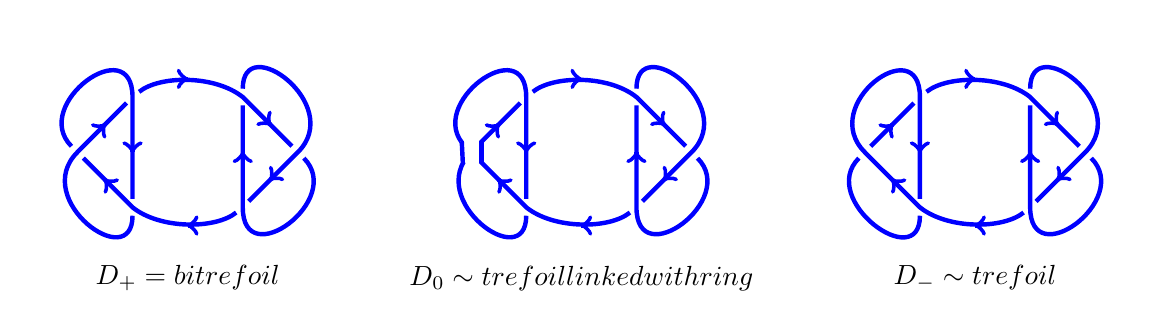
\begin{tikzpicture}
  \begin{scope}
   \begin{scope}[scale=0.7]
    \node (a) at (-1.0, 1) {};
    \node (b) at (-2, 0) {};
    \node (c) at (-1.0,-1) {};
    \node (d) at ( 1.0, 1) {};
    \node (e) at ( 2, 0) {};
    \node (f) at ( 1.0,-1) {};
    \draw (a)        .. controls (-0.5,1.4) and (0.5,1.4) ..
          (d.center) .. controls (d.8 south east) and (e.8 north west) ..
          (e)        .. controls (e.8 south east) and (f.8 south) ..
          (f.center) .. controls (f.8 north) and (d.8 south) ..
          (d)        .. controls (d.8 north) and (e.8 north east) ..
          (e.center) .. controls (e.8 south west) and (f.8 north east) ..
          (f)        .. controls (0.5,-1.4) and (-0.5,-1.4) ..
          (c.center) .. controls (c.8 north west) and (b.8 south east) ..
          (b)        .. controls (b.8 north west) and (a.8 north) ..
          (a.center) .. controls (a.8 south) and (c.8 north) ..
          (c)        .. controls (c.8 south) and (b.8 south west) ..
          (b.center) .. controls (b.8 north east) and (a.8 south west) ..
          (a);
    \draw[->] (0, 1.33) -- +( 0.01,0);
    \draw[->] (0,-1.33) -- +(-0.01,0);
    \draw[->] (-1,0) -- +(0,-0.01);
    \draw[->] ( 1,0) -- +(0, 0.01);
    \draw[->] (-1.5, 0.5) -- + ( 0.01, 0.01);
    \draw[->] (-1.5,-0.5) -- + (-0.01, 0.01);
    \draw[->] ( 1.5, 0.5) -- + ( 0.01,-0.01);
    \draw[->] ( 1.5,-0.5) -- + (-0.01,-0.01);
   \end{scope}
   \draw[black](0,-1.6) node {$D_+=\text{ bitrefoil }$};
  \end{scope}
  \begin{scope}[xshift=5cm]
   \begin{scope}[scale=0.7]
    \node (a) at (-1.0, 1) {};
    \node (b) at (-2, 0) {};
    \node (c) at (-1.0,-1) {};
    \node (d) at ( 1.0, 1) {};
    \node (e) at ( 2, 0) {};
    \node (f) at ( 1.0,-1) {};
    \draw (a)        .. controls (-0.5,1.4) and (0.5,1.4) ..
          (d.center) .. controls (d.8 south east) and (e.8 north west) ..
          (e)        .. controls (e.8 south east) and (f.8 south) ..
          (f.center) .. controls (f.8 north) and (d.8 south) ..
          (d)        .. controls (d.8 north) and (e.8 north east) ..
          (e.center) .. controls (e.8 south west) and (f.8 north east) ..
          (f)        .. controls (0.5,-1.4) and (-0.5,-1.4) ..
          (c.center) .. controls (c.8 north west) and (b.8 south east) ..
          (b)        .. controls (b.8 north west) and (a.8 north) ..
          (a.center) .. controls (a.8 south) and (c.8 north) ..
          (c)        .. controls (c.8 south) and (b.8 south west) ..
          (b.center) .. controls (b.8 north east) and (a.8 south west) ..
          (a);
    \draw[->] (0, 1.33) -- +( 0.01,0);
    \draw[->] (0,-1.33) -- +(-0.01,0);
    \draw[->] (-1,0) -- +(0,-0.01);
    \draw[->] ( 1,0) -- +(0, 0.01);
    \draw[->] (-1.5, 0.5) -- + ( 0.01, 0.01);
    \draw[->] (-1.5,-0.5) -- + (-0.01, 0.01);
    \draw[->] ( 1.5, 0.5) -- + ( 0.01,-0.01);
    \draw[->] ( 1.5,-0.5) -- + (-0.01,-0.01);
    \fill[white] (-2.2,-0.2) rectangle (-1.8, 0.2);
    \draw (-2.17,0.2) -- (-2.15,-0.2);
    \draw (-1.81,0.2) -- (-1.81,-0.2);
   \end{scope}
   \draw[black](0,-1.6) node {$D_0\sim\text{ trefoil linked with ring }$};
  \end{scope}
  \begin{scope}[xshift=10cm]
   \begin{scope}[scale=0.7]
    \node (a) at (-1.0, 1) {};
    \node (b) at (-2, 0) {};
    \node (c) at (-1.0,-1) {};
    \node (d) at ( 1.0, 1) {};
    \node (e) at ( 2, 0) {};
    \node (f) at ( 1.0,-1) {};
    \draw (a)        .. controls (-0.5,1.4) and (0.5,1.4) ..
          (d.center) .. controls (d.8 south east) and (e.8 north west) ..
          (e)        .. controls (e.8 south east) and (f.8 south) ..
          (f.center) .. controls (f.8 north) and (d.8 south) ..
          (d)        .. controls (d.8 north) and (e.8 north east) ..
          (e.center) .. controls (e.8 south west) and (f.8 north east) ..
          (f)        .. controls (0.5,-1.4) and (-0.5,-1.4) ..
          (c.center) .. controls (c.8 north west) and (b.8 south east) ..
          (b.center) .. controls (b.8 north west) and (a.8 north) ..
          (a.center) .. controls (a.8 south) and (c.8 north) ..
          (c)        .. controls (c.8 south) and (b.8 south west) ..
          (b)        .. controls (b.8 north east) and (a.8 south west) ..
          (a);
    \draw[->] (0, 1.33) -- +( 0.01,0);
    \draw[->] (0,-1.33) -- +(-0.01,0);
    \draw[->] (-1,0) -- +(0,-0.01);
    \draw[->] ( 1,0) -- +(0, 0.01);
    \draw[->] (-1.5, 0.5) -- + ( 0.01, 0.01);
    \draw[->] (-1.5,-0.5) -- + (-0.01, 0.01);
    \draw[->] ( 1.5, 0.5) -- + ( 0.01,-0.01);
    \draw[->] ( 1.5,-0.5) -- + (-0.01,-0.01);
   \end{scope}
   \draw[black](0,-1.6) node {$D_-\sim\text{ trefoil }$};
  \end{scope}
 \end{tikzpicture}
\end{center}

\begin{center}
 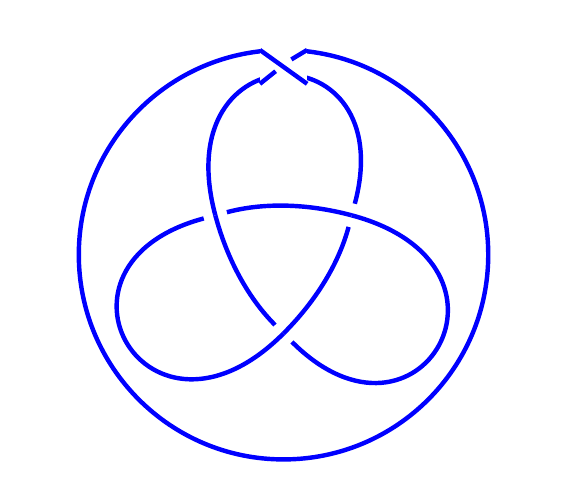
\begin{tikzpicture}
  \draw (0,0) circle(2.6);
  \begin{scope}[rotate=  0] \node (a) at (0,-1) {}; \end{scope}
  \begin{scope}[rotate=120] \node (b) at (0,-1) {}; \end{scope}
  \begin{scope}[rotate=240] \node (c) at (0,-1) {}; \end{scope}
  \draw (a) .. controls (a.4 north west) and (c.4 north east) .. (c.center);
  \draw (b) .. controls (b.4 north west) and (a.4 north east) .. (a.center);
  \draw (c) .. controls (c.4 north west) and (b.4 north east) .. (b.center);
  \draw (a.center) .. controls (a.16 south west) and (c.16 south east) .. (c);
  \draw (b.center) .. controls (b.16 south west) and (a.16 south east) .. (a);
  \draw (c.center) .. controls (c.16 south west) and (b.16 south east) .. (b);
  \fill[white] (-0.3,1.2) rectangle (0.3,2.7);
  \draw (-0.3,2.60) -- (0.3,2.17);
  \draw (-0.3,2.17) -- (-0.1,2.33);
  \draw ( 0.3,2.60) -- ( 0.1,2.48);
 \end{tikzpicture}
\end{center}

\begin{center}
 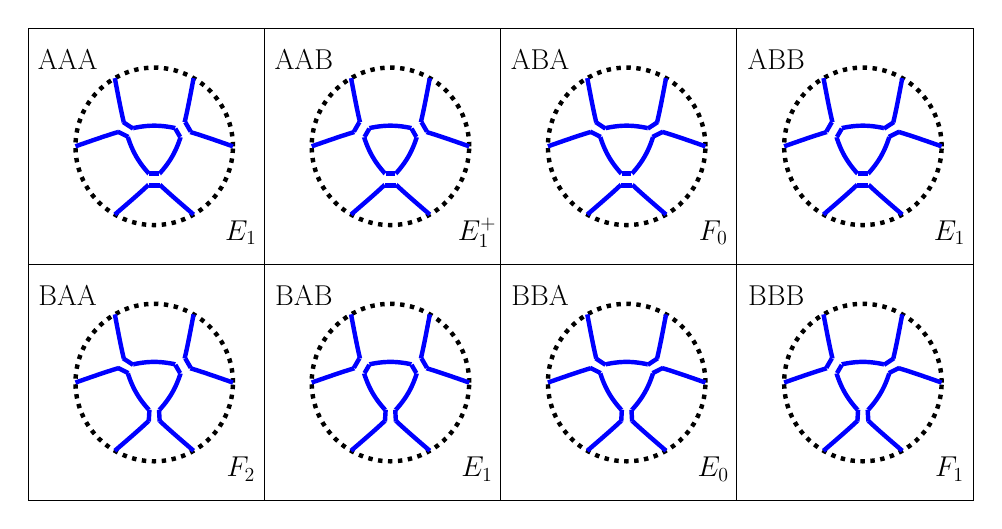
\begin{tikzpicture}
  \draw[thin,black] (-1.6, 1.5) -- (-1.6,-4.5);
  \draw[thin,black] ( 1.4, 1.5) -- ( 1.4,-4.5);
  \draw[thin,black] ( 4.4, 1.5) -- ( 4.4,-4.5);
  \draw[thin,black] ( 7.4, 1.5) -- ( 7.4,-4.5);
  \draw[thin,black] (10.4, 1.5) -- (10.4,-4.5);
  \draw[thin,black] (-1.6, 1.5) -- (10.4, 1.5);
  \draw[thin,black] (-1.6,-1.5) -- (10.4,-1.5);
  \draw[thin,black] (-1.6,-4.5) -- (10.4,-4.5);
  \def\pA{\draw ( 82:-1.00) -- ( 98:-1.00); \draw ( 80:-0.70) -- (100:-0.70);}
  \def\pB{\draw ( 82:-1.00) -- ( 80:-0.70); \draw ( 98:-1.00) -- (100:-0.70);}
  \def\qA{\draw (202:-1.00) -- (218:-1.00); \draw (200:-0.70) -- (220:-0.70);}
  \def\qB{\draw (202:-1.00) -- (200:-0.70); \draw (218:-1.00) -- (220:-0.70);}
  \def\rA{\draw (322:-1.00) -- (320:-0.70); \draw (338:-1.00) -- (340:-0.70);}
  \def\rB{\draw (322:-1.00) -- (338:-1.00); \draw (320:-0.70) -- (340:-0.70);}
  \begin{scope}
   \begin{scope}[scale=0.5]
    \draw[black] (-2.2, 2.2) node{\huge AAA};
    \draw[black] ( 2.2,-2.2) node{\huge $E_1$};
    \draw[black,dotted] (0,0) circle(2);
    \foreach \t in {0,120,240} {
     \begin{scope}[rotate=\t]
      \draw (  0:2) .. controls (270:-0.7) .. (180:2);
     \end{scope}
    }
    \foreach \t in {0,120,240} {
     \begin{scope}[rotate=\t]
      \fill[white] (90:-0.84) circle(0.2);
     \end{scope}
    }
    \pA\qA\rA
   \end{scope}
   \begin{scope}[xshift=3cm,scale=0.5]
    \draw[black] (-2.2, 2.2) node{\huge AAB};
    \draw[black] ( 2.2,-2.2) node{\huge $E_1^+$};
    \draw[black,dotted] (0,0) circle(2);
    \foreach \t in {0,120,240} {
     \begin{scope}[rotate=\t]
      \draw (  0:2) .. controls (270:-0.7) .. (180:2);
     \end{scope}
    }
    \foreach \t in {0,120,240} {
     \begin{scope}[rotate=\t]
      \fill[white] (90:-0.84) circle(0.2);
     \end{scope}
    }
    \pA\qA\rB
   \end{scope}
   \begin{scope}[xshift=6cm,scale=0.5]
    \draw[black] (-2.2, 2.2) node{\huge ABA};
    \draw[black] ( 2.2,-2.2) node{\huge $F_0$};
    \draw[black,dotted] (0,0) circle(2);
    \foreach \t in {0,120,240} {
     \begin{scope}[rotate=\t]
      \draw (  0:2) .. controls (270:-0.7) .. (180:2);
     \end{scope}
    }
    \foreach \t in {0,120,240} {
     \begin{scope}[rotate=\t]
      \fill[white] (90:-0.84) circle(0.2);
     \end{scope}
    }
    \pA\qB\rA
   \end{scope}
   \begin{scope}[xshift=9cm,scale=0.5]
    \draw[black] (-2.2, 2.2) node{\huge ABB};
    \draw[black] ( 2.2,-2.2) node{\huge $E_1$};
    \draw[black,dotted] (0,0) circle(2);
    \foreach \t in {0,120,240} {
     \begin{scope}[rotate=\t]
      \draw (  0:2) .. controls (270:-0.7) .. (180:2);
     \end{scope}
    }
    \foreach \t in {0,120,240} {
     \begin{scope}[rotate=\t]
      \fill[white] (90:-0.84) circle(0.2);
     \end{scope}
    }
    \pA\qB\rB
   \end{scope}
   \begin{scope}[yshift=-3cm,scale=0.5]
    \draw[black] (-2.2, 2.2) node{\huge BAA};
    \draw[black] ( 2.2,-2.2) node{\huge $F_2$};
    \draw[black,dotted] (0,0) circle(2);
    \foreach \t in {0,120,240} {
     \begin{scope}[rotate=\t]
      \draw (  0:2) .. controls (270:-0.7) .. (180:2);
     \end{scope}
    }
    \foreach \t in {0,120,240} {
     \begin{scope}[rotate=\t]
      \fill[white] (90:-0.84) circle(0.2);
     \end{scope}
    }
    \pB\qA\rA
   \end{scope}
   \begin{scope}[yshift=-3cm,xshift=3cm,scale=0.5]
    \draw[black] (-2.2, 2.2) node{\huge BAB};
    \draw[black] ( 2.2,-2.2) node{\huge $E_1$};
    \draw[black,dotted] (0,0) circle(2);
    \foreach \t in {0,120,240} {
     \begin{scope}[rotate=\t]
      \draw (  0:2) .. controls (270:-0.7) .. (180:2);
     \end{scope}
    }
    \foreach \t in {0,120,240} {
     \begin{scope}[rotate=\t]
      \fill[white] (90:-0.84) circle(0.2);
     \end{scope}
    }
    \pB\qA\rB
   \end{scope}
   \begin{scope}[yshift=-3cm,xshift=6cm,scale=0.5]
    \draw[black] (-2.2, 2.2) node{\huge BBA};
    \draw[black] ( 2.2,-2.2) node{\huge $E_0$};
    \draw[black,dotted] (0,0) circle(2);
    \foreach \t in {0,120,240} {
     \begin{scope}[rotate=\t]
      \draw (  0:2) .. controls (270:-0.7) .. (180:2);
     \end{scope}
    }
    \foreach \t in {0,120,240} {
     \begin{scope}[rotate=\t]
      \fill[white] (90:-0.84) circle(0.2);
     \end{scope}
    }
    \pB\qB\rA
   \end{scope}
   \begin{scope}[yshift=-3cm,xshift=9cm,scale=0.5]
    \draw[black] (-2.2, 2.2) node{\huge BBB};
    \draw[black] ( 2.2,-2.2) node{\huge $F_1$};
    \draw[black,dotted] (0,0) circle(2);
    \foreach \t in {0,120,240} {
     \begin{scope}[rotate=\t]
      \draw (  0:2) .. controls (270:-0.7) .. (180:2);
     \end{scope}
    }
    \foreach \t in {0,120,240} {
     \begin{scope}[rotate=\t]
      \fill[white] (90:-0.84) circle(0.2);
     \end{scope}
    }
    \pB\qB\rB
   \end{scope}
  \end{scope}
 \end{tikzpicture}
\end{center}

\begin{center}
 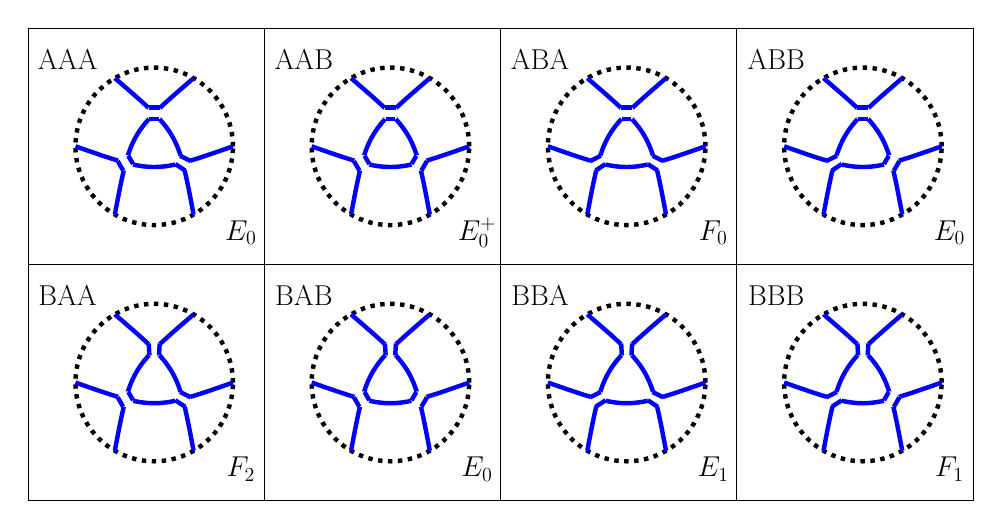
\begin{tikzpicture}
  \draw[thin,black] (-1.6, 1.5) -- (-1.6,-4.5);
  \draw[thin,black] ( 1.4, 1.5) -- ( 1.4,-4.5);
  \draw[thin,black] ( 4.4, 1.5) -- ( 4.4,-4.5);
  \draw[thin,black] ( 7.4, 1.5) -- ( 7.4,-4.5);
  \draw[thin,black] (10.4, 1.5) -- (10.4,-4.5);
  \draw[thin,black] (-1.6, 1.5) -- (10.4, 1.5);
  \draw[thin,black] (-1.6,-1.5) -- (10.4,-1.5);
  \draw[thin,black] (-1.6,-4.5) -- (10.4,-4.5);
  \def\pA{\draw ( 82:1.00) -- ( 98:1.00); \draw ( 80:0.70) -- (100:0.70);}
  \def\pB{\draw ( 82:1.00) -- ( 80:0.70); \draw ( 98:1.00) -- (100:0.70);}
  \def\qA{\draw (202:1.00) -- (218:1.00); \draw (200:0.70) -- (220:0.70);}
  \def\qB{\draw (202:1.00) -- (200:0.70); \draw (218:1.00) -- (220:0.70);}
  \def\rA{\draw (322:1.00) -- (320:0.70); \draw (338:1.00) -- (340:0.70);}
  \def\rB{\draw (322:1.00) -- (338:1.00); \draw (320:0.70) -- (340:0.70);}
  \begin{scope}
   \begin{scope}[scale=0.5]
    \draw[black] (-2.2, 2.2) node{\huge AAA};
    \draw[black] ( 2.2,-2.2) node{\huge $E_0$};
    \draw[black,dotted] (0,0) circle(2);
    \foreach \t in {0,120,240} {
     \begin{scope}[rotate=\t]
      \draw (  0:2) .. controls (270:0.7) .. (180:2);
     \end{scope}
    }
    \foreach \t in {0,120,240} {
     \begin{scope}[rotate=\t]
      \fill[white] (90:0.84) circle(0.2);
     \end{scope}
    }
    \pA\qA\rA
   \end{scope}
   \begin{scope}[xshift=3cm,scale=0.5]
    \draw[black] (-2.2, 2.2) node{\huge AAB};
    \draw[black] ( 2.2,-2.2) node{\huge $E_0^+$};
    \draw[black,dotted] (0,0) circle(2);
    \foreach \t in {0,120,240} {
     \begin{scope}[rotate=\t]
      \draw (  0:2) .. controls (270:0.7) .. (180:2);
     \end{scope}
    }
    \foreach \t in {0,120,240} {
     \begin{scope}[rotate=\t]
      \fill[white] (90:0.84) circle(0.2);
     \end{scope}
    }
    \pA\qA\rB
   \end{scope}
   \begin{scope}[xshift=6cm,scale=0.5]
    \draw[black] (-2.2, 2.2) node{\huge ABA};
    \draw[black] ( 2.2,-2.2) node{\huge $F_0$};
    \draw[black,dotted] (0,0) circle(2);
    \foreach \t in {0,120,240} {
     \begin{scope}[rotate=\t]
      \draw (  0:2) .. controls (270:0.7) .. (180:2);
     \end{scope}
    }
    \foreach \t in {0,120,240} {
     \begin{scope}[rotate=\t]
      \fill[white] (90:0.84) circle(0.2);
     \end{scope}
    }
    \pA\qB\rA
   \end{scope}
   \begin{scope}[xshift=9cm,scale=0.5]
    \draw[black] (-2.2, 2.2) node{\huge ABB};
    \draw[black] ( 2.2,-2.2) node{\huge $E_0$};
    \draw[black,dotted] (0,0) circle(2);
    \foreach \t in {0,120,240} {
     \begin{scope}[rotate=\t]
      \draw (  0:2) .. controls (270:0.7) .. (180:2);
     \end{scope}
    }
    \foreach \t in {0,120,240} {
     \begin{scope}[rotate=\t]
      \fill[white] (90:0.84) circle(0.2);
     \end{scope}
    }
    \pA\qB\rB
   \end{scope}
   \begin{scope}[yshift=-3cm,scale=0.5]
    \draw[black] (-2.2, 2.2) node{\huge BAA};
    \draw[black] ( 2.2,-2.2) node{\huge $F_2$};
    \draw[black,dotted] (0,0) circle(2);
    \foreach \t in {0,120,240} {
     \begin{scope}[rotate=\t]
      \draw (  0:2) .. controls (270:0.7) .. (180:2);
     \end{scope}
    }
    \foreach \t in {0,120,240} {
     \begin{scope}[rotate=\t]
      \fill[white] (90:0.84) circle(0.2);
     \end{scope}
    }
    \pB\qA\rA
   \end{scope}
   \begin{scope}[yshift=-3cm,xshift=3cm,scale=0.5]
    \draw[black] (-2.2, 2.2) node{\huge BAB};
    \draw[black] ( 2.2,-2.2) node{\huge $E_0$};
    \draw[black,dotted] (0,0) circle(2);
    \foreach \t in {0,120,240} {
     \begin{scope}[rotate=\t]
      \draw (  0:2) .. controls (270:0.7) .. (180:2);
     \end{scope}
    }
    \foreach \t in {0,120,240} {
     \begin{scope}[rotate=\t]
      \fill[white] (90:0.84) circle(0.2);
     \end{scope}
    }
    \pB\qA\rB
   \end{scope}
   \begin{scope}[yshift=-3cm,xshift=6cm,scale=0.5]
    \draw[black] (-2.2, 2.2) node{\huge BBA};
    \draw[black] ( 2.2,-2.2) node{\huge $E_1$};
    \draw[black,dotted] (0,0) circle(2);
    \foreach \t in {0,120,240} {
     \begin{scope}[rotate=\t]
      \draw (  0:2) .. controls (270:0.7) .. (180:2);
     \end{scope}
    }
    \foreach \t in {0,120,240} {
     \begin{scope}[rotate=\t]
      \fill[white] (90:0.84) circle(0.2);
     \end{scope}
    }
    \pB\qB\rA
   \end{scope}
   \begin{scope}[yshift=-3cm,xshift=9cm,scale=0.5]
    \draw[black] (-2.2, 2.2) node{\huge BBB};
    \draw[black] ( 2.2,-2.2) node{\huge $F_1$};
    \draw[black,dotted] (0,0) circle(2);
    \foreach \t in {0,120,240} {
     \begin{scope}[rotate=\t]
      \draw (  0:2) .. controls (270:0.7) .. (180:2);
     \end{scope}
    }
    \foreach \t in {0,120,240} {
     \begin{scope}[rotate=\t]
      \fill[white] (90:0.84) circle(0.2);
     \end{scope}
    }
    \pB\qB\rB
   \end{scope}
  \end{scope}
 \end{tikzpicture}
\end{center}

\begin{center}
 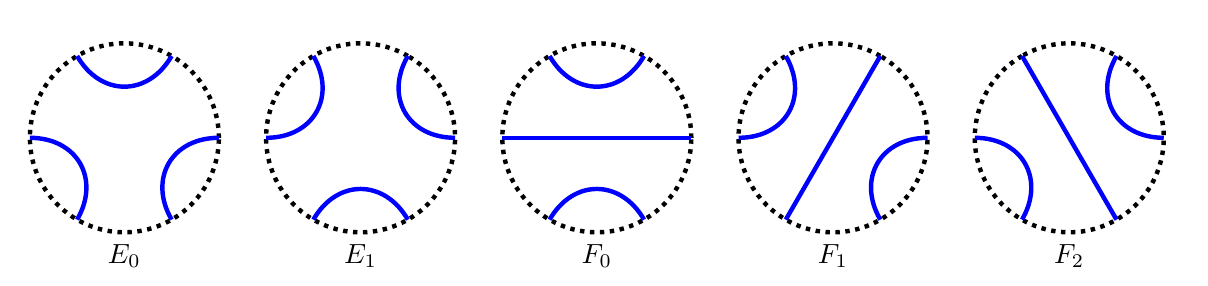
\begin{tikzpicture}
  \begin{scope}[scale=0.6]
   \draw[black,dotted] (0,0) circle(2);
   \draw ( 60:2) .. controls ( 60:1) and (120:1) .. (120:2);
   \draw (180:2) .. controls (180:1) and (240:1) .. (240:2);
   \draw (300:2) .. controls (300:1) and (360:1) .. (360:2);
  \end{scope}
  \begin{scope}[xshift=3cm,rotate=60,scale=0.6]
   \draw[black,dotted] (0,0) circle(2);
   \draw ( 60:2) .. controls ( 60:1) and (120:1) .. (120:2);
   \draw (180:2) .. controls (180:1) and (240:1) .. (240:2);
   \draw (300:2) .. controls (300:1) and (360:1) .. (360:2);
  \end{scope}
  \begin{scope}[xshift=6cm,scale=0.6]
   \draw[black,dotted] (0,0) circle(2);
   \draw ( 60:2) .. controls ( 60:1) and (120:1) .. (120:2);
   \draw (180:2) -- (  0:2);
   \draw (-60:2) .. controls (-60:1) and (240:1) .. (240:2);
  \end{scope}
  \begin{scope}[xshift=9cm,rotate=60,scale=0.6]
   \draw[black,dotted] (0,0) circle(2);
   \draw ( 60:2) .. controls ( 60:1) and (120:1) .. (120:2);
   \draw (180:2) -- (  0:2);
   \draw (-60:2) .. controls (-60:1) and (240:1) .. (240:2);
  \end{scope}
  \begin{scope}[xshift=12cm,rotate=120,scale=0.6]
   \draw[black,dotted] (0,0) circle(2);
   \draw ( 60:2) .. controls ( 60:1) and (120:1) .. (120:2);
   \draw (180:2) -- (  0:2);
   \draw (-60:2) .. controls (-60:1) and (240:1) .. (240:2);
  \end{scope}
  \draw[black] ( 0,-1.5) node{$E_0$};
  \draw[black] ( 3,-1.5) node{$E_1$};
  \draw[black] ( 6,-1.5) node{$F_0$};
  \draw[black] ( 9,-1.5) node{$F_1$};
  \draw[black] (12,-1.5) node{$F_2$};
 \end{tikzpicture}
\end{center}

\begin{center}
 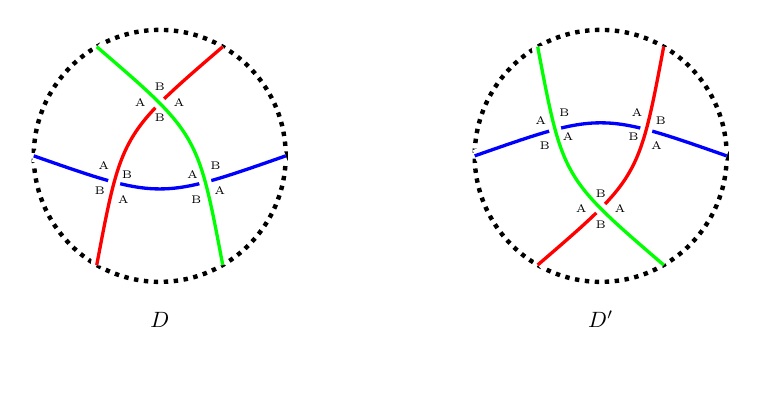
\begin{tikzpicture}[scale=0.8]
  \begin{scope}
   \draw[black,dotted] (0,0) circle(2);
   \draw[draw=white,double=blue ,ultra thick,double distance=1.2pt] (  0:2) .. controls (270:0.7) .. (180:2);
   \draw[draw=white,double=red  ,ultra thick,double distance=1.2pt] ( 60:2) .. controls (150:0.7) .. (240:2);
   \draw[draw=white,double=green,ultra thick,double distance=1.2pt] (120:2) .. controls ( 30:0.7) .. (300:2);
   \draw[black] ( 90: 1.1) node {\tiny B}; \draw[black] ( 90: 0.6) node {\tiny B};
   \draw[black] (210: 1.1) node {\tiny B}; \draw[black] (210: 0.6) node {\tiny B};
   \draw[black] (330: 1.1) node {\tiny A}; \draw[black] (330: 0.6) node {\tiny A};
   \draw[black] (-10: 0.9) node {\tiny B};
   \draw[black] ( 70: 0.9) node {\tiny A};
   \draw[black] (110: 0.9) node {\tiny A};
   \draw[black] (190: 0.9) node {\tiny A};
   \draw[black] (230: 0.9) node {\tiny A};
   \draw[black] (310: 0.9) node {\tiny B};
   \draw[black] (0,-2.6) node {$D$};
   \draw[white] (-2,-3.3) -- (2,-3.3);
  \end{scope}
  \begin{scope}[xshift=7cm]
   \draw[black,dotted] (0,0) circle(2);
   \draw[draw=white,double=blue ,ultra thick,double distance=1.2pt] (  0:2) .. controls ( 90:0.7) .. (180:2);
   \draw[draw=white,double=red  ,ultra thick,double distance=1.2pt] ( 60:2) .. controls (330:0.7) .. (240:2);
   \draw[draw=white,double=green,ultra thick,double distance=1.2pt] (120:2) .. controls (210:0.7) .. (300:2);
   \draw[black] ( 90:-1.1) node {\tiny B}; \draw[black] ( 90:-0.6) node {\tiny B};
   \draw[black] (210:-1.1) node {\tiny B}; \draw[black] (210:-0.6) node {\tiny B};
   \draw[black] (330:-1.1) node {\tiny A}; \draw[black] (330:-0.6) node {\tiny A};
   \draw[black] (-10:-0.9) node {\tiny B};
   \draw[black] ( 70:-0.9) node {\tiny A};
   \draw[black] (110:-0.9) node {\tiny A};
   \draw[black] (190:-0.9) node {\tiny A};
   \draw[black] (230:-0.9) node {\tiny A};
   \draw[black] (310:-0.9) node {\tiny B};
   \draw[black] (0,-2.6) node {$D'$};
   \draw[white] (-2,-3.3) -- (2,-3.3);
  \end{scope}
 \end{tikzpicture}
\end{center}

\begin{center}
 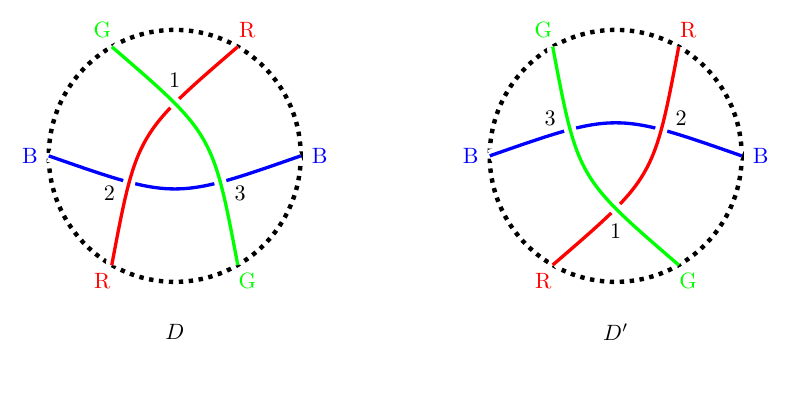
\begin{tikzpicture}[scale=0.8]
  \begin{scope}
   \draw[black,dotted] (0,0) circle(2);
   \draw[draw=white,double=blue ,ultra thick,double distance=1.2pt] (  0:2) .. controls (270:0.7) .. (180:2);
   \draw[draw=white,double=red  ,ultra thick,double distance=1.2pt] ( 60:2) .. controls (150:0.7) .. (240:2);
   \draw[draw=white,double=green,ultra thick,double distance=1.2pt] (120:2) .. controls ( 30:0.7) .. (300:2);
   \draw[red  ] ( 60: 2.3) node {R};  \draw[red  ] ( 60:-2.3) node {R};
   \draw[blue ] (180: 2.3) node {B};  \draw[blue ] (180:-2.3) node {B};
   \draw[green] (300: 2.3) node {G};  \draw[green] (300:-2.3) node {G};
   \draw[black] ( 90: 1.2) node {1};
   \draw[black] (210: 1.2) node {2};
   \draw[black] (330: 1.2) node {3};
   \draw[black] (0,-2.8) node {$D$};
   \draw[white] (-2,-3.3) -- (2,-3.3);
  \end{scope}
  \begin{scope}[xshift=7cm]
   \draw[black,dotted] (0,0) circle(2);
   \draw[draw=white,double=blue ,ultra thick,double distance=1.2pt] (  0:2) .. controls ( 90:0.7) .. (180:2);
   \draw[draw=white,double=red  ,ultra thick,double distance=1.2pt] ( 60:2) .. controls (330:0.7) .. (240:2);
   \draw[draw=white,double=green,ultra thick,double distance=1.2pt] (120:2) .. controls (210:0.7) .. (300:2);
   \draw[red  ] ( 60: 2.3) node {R};  \draw[red  ] ( 60:-2.3) node {R};
   \draw[blue ] (180: 2.3) node {B};  \draw[blue ] (180:-2.3) node {B};
   \draw[green] (300: 2.3) node {G};  \draw[green] (300:-2.3) node {G};
   \draw[black] ( 90:-1.2) node {1};
   \draw[black] (210:-1.2) node {2};
   \draw[black] (330:-1.2) node {3};
   \draw[black] (0,-2.8) node {$D'$};
   \draw[white] (-2,-3.3) -- (2,-3.3);
  \end{scope}
 \end{tikzpicture}
\end{center}


\begin{center}
 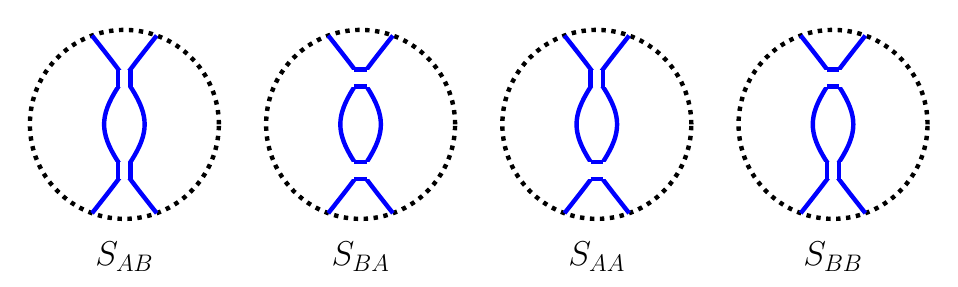
\begin{tikzpicture}[scale=0.6]
  \begin{scope}
   \draw[black,dotted] (0,0) circle(2);
   \draw (110:2) .. controls ( 0.8,0) .. (250:2); 
   \draw ( 70:2) .. controls (-0.8,0) .. (290:2);
   \fill[white] (-0.20, 0.80) rectangle (0.20, 1.16);
   \fill[white] (-0.20,-0.80) rectangle (0.20,-1.16);
   \draw (-0.13, 0.80) -- (-0.13, 1.16);
   \draw ( 0.13, 0.80) -- ( 0.13, 1.16);
   \draw (-0.13,-0.80) -- (-0.13,-1.16);
   \draw ( 0.13,-0.80) -- ( 0.13,-1.16);
   \draw[black] ( 0.0,-2.8) node {\huge $S_{AB}$};
  \end{scope}
  \begin{scope}[xshift=5cm]
   \draw[black,dotted] (0,0) circle(2);
   \draw (110:2) .. controls ( 0.8,0) .. (250:2); 
   \draw ( 70:2) .. controls (-0.8,0) .. (290:2);
   \fill[white] (-0.20, 0.80) rectangle (0.20, 1.16);
   \fill[white] (-0.20,-0.80) rectangle (0.20,-1.16);
   \draw (-0.13, 1.16) -- ( 0.13, 1.16);
   \draw (-0.13, 0.80) -- ( 0.13, 0.80);
   \draw (-0.13,-1.16) -- ( 0.13,-1.16);
   \draw (-0.13,-0.80) -- ( 0.13,-0.80);
   \draw[black] ( 0.0,-2.8) node {\huge $S_{BA}$};
  \end{scope}
  \begin{scope}[xshift=10cm]
   \draw[black,dotted] (0,0) circle(2);
   \draw (110:2) .. controls ( 0.8,0) .. (250:2); 
   \draw ( 70:2) .. controls (-0.8,0) .. (290:2);
   \fill[white] (-0.20, 0.80) rectangle (0.20, 1.16);
   \fill[white] (-0.20,-0.80) rectangle (0.20,-1.16);
   \draw (-0.13, 0.80) -- (-0.13, 1.16);
   \draw ( 0.13, 0.80) -- ( 0.13, 1.16);
   \draw (-0.13,-1.16) -- ( 0.13,-1.16);
   \draw (-0.13,-0.80) -- ( 0.13,-0.80);
   \draw[black] ( 0.0,-2.8) node {\huge $S_{AA}$};
  \end{scope}
  \begin{scope}[xshift=15cm]
   \draw[black,dotted] (0,0) circle(2);
   \draw (110:2) .. controls ( 0.8,0) .. (250:2); 
   \draw ( 70:2) .. controls (-0.8,0) .. (290:2);
   \fill[white] (-0.20, 0.80) rectangle (0.20, 1.16);
   \fill[white] (-0.20,-0.80) rectangle (0.20,-1.16);
   \draw[black] ( 0.0,-2.8) node {\huge $S_{BB}$};
   \draw (-0.13, 1.16) -- ( 0.13, 1.16);
   \draw (-0.13, 0.80) -- ( 0.13, 0.80);
   \draw (-0.13,-0.80) -- (-0.13,-1.16);
   \draw ( 0.13,-0.80) -- ( 0.13,-1.16);
  \end{scope}
 \end{tikzpicture}
\end{center}

\begin{center}
 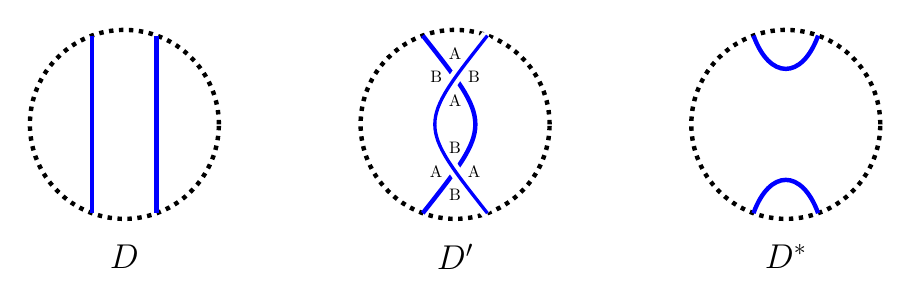
\begin{tikzpicture}[scale=0.6]
  \begin{scope}
   \draw[black,dotted] (0,0) circle(2);
   \draw (110:2) -- (250:2);
   \draw ( 70:2) -- (290:2);
   \draw[black] (0,-2.8) node {\huge $D$};
  \end{scope}
  \begin{scope}[xshift=7cm]
   \draw[black,dotted] (0,0) circle(2);
   \draw (110:2) .. controls ( 0.8,0) .. (250:2); 
   \draw[draw=white,double=blue,ultra thick,double distance=1.2pt] ( 70:2) .. controls (-0.8,0) .. (290:2);
   \draw[black] ( 0.0, 1.5) node {A};
   \draw[black] ( 0.0, 0.5) node {A};
   \draw[black] ( 0.0,-0.5) node {B};
   \draw[black] ( 0.0,-1.5) node {B};
   \draw[black] ( 0.4, 1.0) node {B};
   \draw[black] ( 0.4,-1.0) node {A};
   \draw[black] (-0.4, 1.0) node {B};
   \draw[black] (-0.4,-1.0) node {A};
   \draw[black] ( 0.0,-2.8) node {\huge $D'$};
  \end{scope}
  \begin{scope}[xshift=14cm]
   \draw[black,dotted] (0,0) circle(2);
   \draw (110:2) .. controls (110:1) and ( 70:1) .. ( 70:2); 
   \draw (250:2) .. controls (250:1) and (290:1) .. (290:2); 
   \draw[black] (0,-2.8) node {\huge $D^*$};
  \end{scope}
 \end{tikzpicture}
\end{center}


\begin{center}
 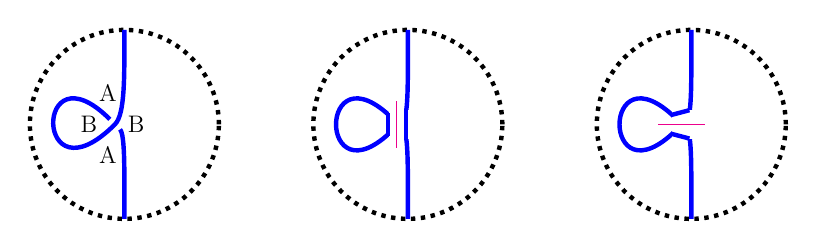
\begin{tikzpicture}[scale=0.6]
  \begin{scope}
   \node (a) at (-0.2,0) {};
   \draw[black,dotted] (0,0) circle(2);
   \draw 
    (0,2) .. controls (0,1) and (a.2 north east) ..
    (a.center) .. controls (a.16 south west) and (a.16 north west) ..
    (a) .. controls (a.2 south east) and (0,-1) ..
    (0,-2);
   \draw[black] (-0.75, 0.00) node {\Large B};
   \draw[black] ( 0.25, 0.00) node {\Large B};
   \draw[black] (-0.35, 0.65) node {\Large A};
   \draw[black] (-0.35,-0.65) node {\Large A};
  \end{scope}
  \begin{scope}[xshift=6cm]
   \node (a) at (-0.2,0) {};
   \draw[black,dotted] (0,0) circle(2);
   \draw 
    (0,2) .. controls (0,1) and (a.2 north east) ..
    (a) .. controls (a.16 south west) and (a.16 north west) ..
    (a) .. controls (a.2 south east) and (0,-1) ..
    (0,-2);
   \fill[white] (-0.4,-0.3) rectangle (0.3,0.3);
   \draw (-0.42,0.24) -- (-0.42,-0.24);
   \draw (-0.04,0.30) -- (-0.04,-0.30);
   \draw[thin,magenta] (-0.24,-0.5) -- (-0.24,0.5);
  \end{scope}
  \begin{scope}[xshift=12cm]
   \node (a) at (-0.2,0) {};
   \draw[black,dotted] (0,0) circle(2);
   \draw 
    (0,2) .. controls (0,1) and (a.2 north east) ..
    (a) .. controls (a.16 south west) and (a.16 north west) ..
    (a) .. controls (a.2 south east) and (0,-1) ..
    (0,-2);
   \fill[white] (-0.4,-0.3) rectangle (0.3,0.3);
   \draw (-0.42, 0.20) -- (-0.04, 0.30);
   \draw (-0.42,-0.20) -- (-0.04,-0.30);
   \draw[thin,magenta] (-0.7,0) -- (0.3,0);
  \end{scope}
 \end{tikzpicture}
\end{center} 

\begin{center}
 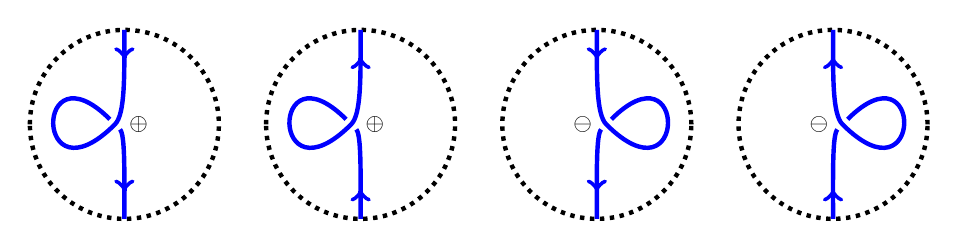
\begin{tikzpicture}[scale=0.6]
  \begin{scope}[xscale=-1]
   \node (a) at (0.2,0) {};
   \draw[black,dotted] (0,0) circle(2);
   \draw 
    (0,2) .. controls (0,1) and (a.2 north west) ..
    (a.center) .. controls (a.16 south east) and (a.16 north east) ..
    (a) .. controls (a.2 south west) and (0,-1) ..
    (0,-2);
   \draw[->] (0, 1.4) -- +(0,-0.01); 
   \draw[->] (0,-1.4) -- +(0,-0.01); 
   \draw[black] (-0.3,0) node {\Large $\oplus$};
  \end{scope}
  \begin{scope}[xshift=5cm,xscale=-1]
   \node (a) at (0.2,0) {};
   \draw[black,dotted] (0,0) circle(2);
   \draw 
    (0,2) .. controls (0,1) and (a.2 north west) ..
    (a.center) .. controls (a.16 south east) and (a.16 north east) ..
    (a) .. controls (a.2 south west) and (0,-1) ..
    (0,-2);
   \draw[->] (0, 1.4) -- +(0, 0.01); 
   \draw[->] (0,-1.4) -- +(0, 0.01); 
   \draw[black] (-0.3,0) node {\Large $\oplus$};
  \end{scope}
  \begin{scope}[xshift=10cm]
   \node (a) at (0.2,0) {};
   \draw[black,dotted] (0,0) circle(2);
   \draw 
    (0,2) .. controls (0,1) and (a.2 north west) ..
    (a.center) .. controls (a.16 south east) and (a.16 north east) ..
    (a) .. controls (a.2 south west) and (0,-1) ..
    (0,-2);
   \draw[->] (0, 1.4) -- +(0,-0.01); 
   \draw[->] (0,-1.4) -- +(0,-0.01); 
   \draw[black] (-0.3,0) node {\Large $\ominus$};
  \end{scope}
  \begin{scope}[xshift=15cm]
   \node (a) at (0.2,0) {};
   \draw[black,dotted] (0,0) circle(2);
   \draw 
    (0,2) .. controls (0,1) and (a.2 north west) ..
    (a.center) .. controls (a.16 south east) and (a.16 north east) ..
    (a) .. controls (a.2 south west) and (0,-1) ..
    (0,-2);
   \draw[->] (0, 1.4) -- +(0, 0.01); 
   \draw[->] (0,-1.4) -- +(0, 0.01); 
   \draw[black] (-0.3,0) node {\Large $\ominus$};
  \end{scope}
 \end{tikzpicture}
\end{center}

\begin{center}
 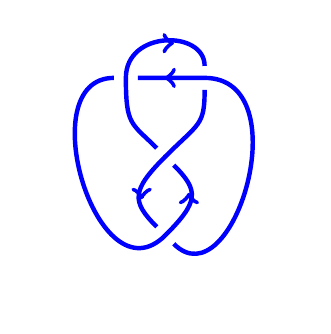
\begin{tikzpicture}
  \node (a) at (-0.50, 1.00) {};
  \node (b) at ( 0.50, 1.00) {};
  \node (c) at ( 0.00, 0.00) {};
  \node (d) at ( 0.00,-1.00) {};
  \draw (a) -- (b.center) 
   .. controls (b.8 east) and (d.8 south east) .. (d)
   .. controls (d.4 north west) and (c.4 south west) .. (c.center)
   .. controls (c.4 north east) and (b.4 south) .. (b)
   .. controls (b.4 north) and (a.4 north) .. (a.center)
   .. controls (a.4 south) and (c.4 north west) .. (c)
   .. controls (c.4 south east) and (d.4 north east) ..(d.center)
   .. controls (d.8 south west) and (a.8 west) .. (a); 
  \draw[->] ( 0.1, 1.44) -- +( 0.01,0); 
  \draw[->] ( 0.0, 1.00) -- +(-0.01,0); 
  \draw[->] ( 0.3,-0.47) -- +( 0, 0.01); 
  \draw[->] (-0.3,-0.53) -- +( 0,-0.01); 
 \end{tikzpicture}
\end{center}

\begin{center}
 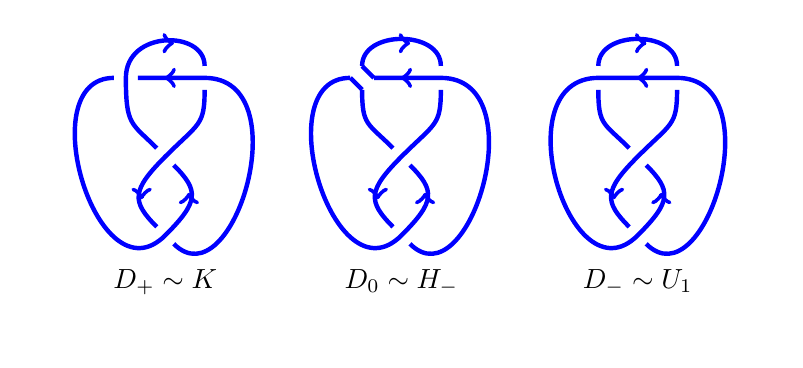
\begin{tikzpicture}
  \begin{scope}
   \node (a) at (-0.50, 1.00) {};
   \node (b) at ( 0.50, 1.00) {};
   \node (c) at ( 0.00, 0.00) {};
   \node (d) at ( 0.00,-1.00) {};
   \draw (a) -- (b.center) 
    .. controls (b.8 east) and (d.8 south east) .. (d)
    .. controls (d.4 north west) and (c.4 south west) .. (c.center)
    .. controls (c.4 north east) and (b.4 south) .. (b)
    .. controls (b.4 north) and (a.4 north) .. (a.center)
    .. controls (a.4 south) and (c.4 north west) .. (c)
    .. controls (c.4 south east) and (d.4 north east) ..(d.center)
    .. controls (d.8 south west) and (a.8 west) .. (a); 
   \draw[->] ( 0.1, 1.44) -- +( 0.01,0); 
   \draw[->] ( 0.0, 1.00) -- +(-0.01,0); 
   \draw[->] ( 0.3,-0.47) -- +( 0, 0.01); 
   \draw[->] (-0.3,-0.53) -- +( 0,-0.01); 
  \end{scope}
  \begin{scope}[xshift=3cm]
   \node (a) at (-0.50, 1.00) {};
   \node (b) at ( 0.50, 1.00) {};
   \node (c) at ( 0.00, 0.00) {};
   \node (d) at ( 0.00,-1.00) {};
   \draw (a) -- (b.center) 
    .. controls (b.8 east) and (d.8 south east) .. (d)
    .. controls (d.4 north west) and (c.4 south west) .. (c.center)
    .. controls (c.4 north east) and (b.4 south) .. (b)
    .. controls (b.4 north) and (a.4 north) .. (a)
    .. controls (a.4 south) and (c.4 north west) .. (c)
    .. controls (c.4 south east) and (d.4 north east) ..(d.center)
    .. controls (d.8 south west) and (a.8 west) .. (a); 
   \draw (-0.35,1.00) -- (-0.50,1.15);
   \draw (-0.65,1.00) -- (-0.50,0.85);
   \draw[->] ( 0.1, 1.44) -- +( 0.01,0); 
   \draw[->] ( 0.0, 1.00) -- +(-0.01,0); 
   \draw[->] ( 0.3,-0.47) -- +( 0, 0.01); 
   \draw[->] (-0.3,-0.53) -- +( 0,-0.01); 
  \end{scope}
  \begin{scope}[xshift=6cm]
   \node (a) at (-0.50, 1.00) {};
   \node (b) at ( 0.50, 1.00) {};
   \node (c) at ( 0.00, 0.00) {};
   \node (d) at ( 0.00,-1.00) {};
   \draw (a.center) -- (b.center) 
    .. controls (b.8 east) and (d.8 south east) .. (d)
    .. controls (d.4 north west) and (c.4 south west) .. (c.center)
    .. controls (c.4 north east) and (b.4 south) .. (b)
    .. controls (b.4 north) and (a.4 north) .. (a)
    .. controls (a.4 south) and (c.4 north west) .. (c)
    .. controls (c.4 south east) and (d.4 north east) ..(d.center)
    .. controls (d.8 south west) and (a.8 west) .. (a.center); 
   \draw[->] ( 0.1, 1.44) -- +( 0.01,0); 
   \draw[->] ( 0.0, 1.00) -- +(-0.01,0); 
   \draw[->] ( 0.3,-0.47) -- +( 0, 0.01); 
   \draw[->] (-0.3,-0.53) -- +( 0,-0.01); 
  \end{scope}
  \draw[black] (0,-1.6) node {$D_+\sim K$};
  \draw[black] (3,-1.6) node {$D_0\sim H_-$};
  \draw[black] (6,-1.6) node {$D_-\sim U_1$};
  \draw[white] (0,-2.3) -- (6,-2);
 \end{tikzpicture}
\end{center}

\begin{center}
 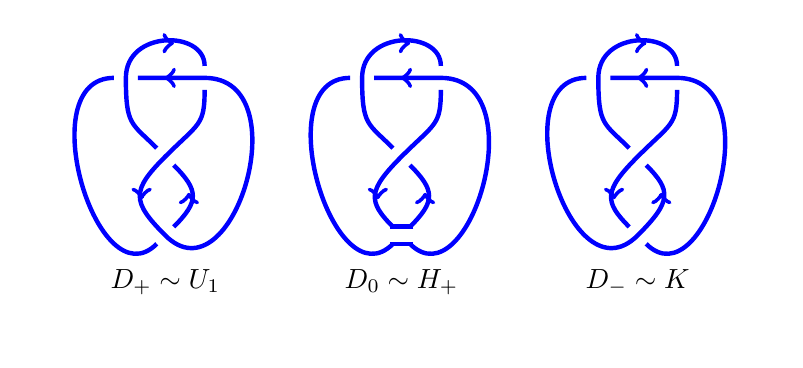
\begin{tikzpicture}
  \begin{scope}
   \node (a) at (-0.50, 1.00) {};
   \node (b) at ( 0.50, 1.00) {};
   \node (c) at ( 0.00, 0.00) {};
   \node (d) at ( 0.00,-1.00) {};
   \draw (a) -- (b.center) 
    .. controls (b.8 east) and (d.8 south east) .. (d.center)
    .. controls (d.4 north west) and (c.4 south west) .. (c.center)
    .. controls (c.4 north east) and (b.4 south) .. (b)
    .. controls (b.4 north) and (a.4 north) .. (a.center)
    .. controls (a.4 south) and (c.4 north west) .. (c)
    .. controls (c.4 south east) and (d.4 north east) ..(d)
    .. controls (d.8 south west) and (a.8 west) .. (a); 
   \draw[->] ( 0.1, 1.44) -- +( 0.01,0); 
   \draw[->] ( 0.0, 1.00) -- +(-0.01,0); 
   \draw[->] ( 0.3,-0.47) -- +( 0, 0.01); 
   \draw[->] (-0.3,-0.53) -- +( 0,-0.01); 
  \end{scope}
  \begin{scope}[xshift=3cm]
   \node (a) at (-0.50, 1.00) {};
   \node (b) at ( 0.50, 1.00) {};
   \node (c) at ( 0.00, 0.00) {};
   \node (d) at ( 0.00,-1.00) {};
   \draw (a) -- (b.center) 
    .. controls (b.8 east) and (d.8 south east) .. (d)
    .. controls (d.4 north west) and (c.4 south west) .. (c.center)
    .. controls (c.4 north east) and (b.4 south) .. (b)
    .. controls (b.4 north) and (a.4 north) .. (a.center)
    .. controls (a.4 south) and (c.4 north west) .. (c)
    .. controls (c.4 south east) and (d.4 north east) ..(d)
    .. controls (d.8 south west) and (a.8 west) .. (a); 
   \draw ( 0.15,-0.89) -- (-0.15,-0.89);
   \draw ( 0.15,-1.11) -- (-0.15,-1.11);
   \draw[->] ( 0.1, 1.44) -- +( 0.01,0); 
   \draw[->] ( 0.0, 1.00) -- +(-0.01,0); 
   \draw[->] ( 0.3,-0.47) -- +( 0, 0.01); 
   \draw[->] (-0.3,-0.53) -- +( 0,-0.01); 
  \end{scope}
  \begin{scope}[xshift=6cm]
   \node (a) at (-0.50, 1.00) {};
   \node (b) at ( 0.50, 1.00) {};
   \node (c) at ( 0.00, 0.00) {};
   \node (d) at ( 0.00,-1.00) {};
   \draw (a) -- (b.center) 
    .. controls (b.8 east) and (d.8 south east) .. (d)
    .. controls (d.4 north west) and (c.4 south west) .. (c.center)
    .. controls (c.4 north east) and (b.4 south) .. (b)
    .. controls (b.4 north) and (a.4 north) .. (a.center)
    .. controls (a.4 south) and (c.4 north west) .. (c)
    .. controls (c.4 south east) and (d.4 north east) ..(d.center)
    .. controls (d.8 south west) and (a.8 west) .. (a); 
   \draw[->] ( 0.1, 1.44) -- +( 0.01,0); 
   \draw[->] ( 0.0, 1.00) -- +(-0.01,0); 
   \draw[->] ( 0.3,-0.47) -- +( 0, 0.01); 
   \draw[->] (-0.3,-0.53) -- +( 0,-0.01); 
  \end{scope}
  \draw[black] (0,-1.6) node {$D_+\sim U_1$};
  \draw[black] (3,-1.6) node {$D_0\sim H_+$};
  \draw[black] (6,-1.6) node {$D_-\sim K$};
  \draw[white] (0,-2.3) -- (6,-2);
 \end{tikzpicture}
\end{center}


 \begin{center}
  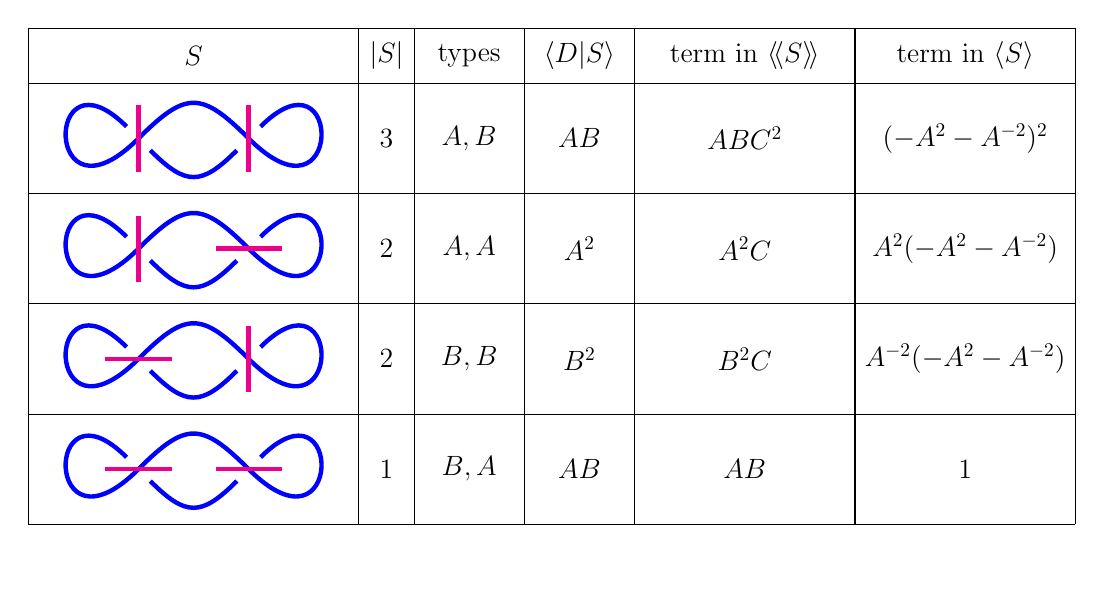
\begin{tikzpicture}[scale=0.7]
   \draw[thin,black] (-3.0, 2) -- (16.0, 2);
   \draw[thin,black] (-3.0, 1) -- (16.0, 1);
   \draw[thin,black] (-3.0,-1) -- (16.0,-1);
   \draw[thin,black] (-3.0,-3) -- (16.0,-3);
   \draw[thin,black] (-3.0,-5) -- (16.0,-5);
   \draw[thin,black] (-3.0,-7) -- (16.0,-7);
   \draw[thin,black] (-3.0, 2) -- (-3.0,-7);
   \draw[thin,black] ( 3.0, 2) -- ( 3.0,-7);
   \draw[thin,black] ( 4.0, 2) -- ( 4.0,-7);
   \draw[thin,black] ( 6.0, 2) -- ( 6.0,-7);
   \draw[thin,black] ( 8.0, 2) -- ( 8.0,-7);
   \draw[thin,black] (12.0, 2) -- (12.0,-7);
   \draw[thin,black] (16.0, 2) -- (16.0,-7);
   \draw[black] ( 0.0,1.5) node {\Large $S$};
   \draw[black] ( 3.5,1.5) node {\Large $|S|$};
   \draw[black] ( 5.0,1.5) node {\Large types};
   \draw[black] ( 7.0,1.5) node {\Large $\ip{D|S}$};
   \draw[black] (10.0,1.5) node {\Large term in $\un{S}$};
   \draw[black] (14.0,1.5) node {\Large term in $\ip{S}$};
   \draw[black] ( 3.5, 0) node {\Large $3$};
   \draw[black] ( 3.5,-2) node {\Large $2$};
   \draw[black] ( 3.5,-4) node {\Large $2$};
   \draw[black] ( 3.5,-6) node {\Large $1$};
   \draw[black] ( 5.0, 0) node {\Large $A,B$};
   \draw[black] ( 5.0,-2) node {\Large $A,A$};
   \draw[black] ( 5.0,-4) node {\Large $B,B$};
   \draw[black] ( 5.0,-6) node {\Large $B,A$};
   \draw[black] ( 7.0, 0) node {\Large $AB$};
   \draw[black] ( 7.0,-2) node {\Large $A^2$};
   \draw[black] ( 7.0,-4) node {\Large $B^2$};
   \draw[black] ( 7.0,-6) node {\Large $AB$};
   \draw[black] (10.0, 0) node {\Large $ABC^2$};
   \draw[black] (10.0,-2) node {\Large $A^2C$};
   \draw[black] (10.0,-4) node {\Large $B^2C$};
   \draw[black] (10.0,-6) node {\Large $AB$};
   \draw[black] (14.0, 0) node {\Large $(-A^2-A^{-2})^2$};
   \draw[black] (14.0,-2) node {\Large $A^2(-A^2-A^{-2})$};
   \draw[black] (14.0,-4) node {\Large $A^{-2}(-A^2-A^{-2})$};
   \draw[black] (14.0,-6) node {\Large $1$};

   \begin{scope}[scale=2]
    \node (a) at (-0.5,0) {};
    \node (b) at ( 0.5,0) {};
    \draw 
     (a.center) .. controls (a.4 north east) and (b.4 north west) ..
     (b.center) .. controls (b.8 south east) and (b.8 north east) ..
     (b)        .. controls (b.4 south west) and (a.4 south east) ..
     (a)        .. controls (a.8 north west) and (a.8 south west) ..
     (a.center);
    \draw[magenta] (-0.5,-0.3) -- (-0.5,0.3);
    \draw[magenta] ( 0.5,-0.3) -- ( 0.5,0.3);
   \end{scope}
   \begin{scope}[scale=2,yshift=-1cm]
    \node (a) at (-0.5,0) {};
    \node (b) at ( 0.5,0) {};
    \draw 
     (a.center) .. controls (a.4 north east) and (b.4 north west) ..
     (b.center) .. controls (b.8 south east) and (b.8 north east) ..
     (b)        .. controls (b.4 south west) and (a.4 south east) ..
     (a)        .. controls (a.8 north west) and (a.8 south west) ..
     (a.center);
    \draw[magenta] (-0.5,-0.3) -- (-0.5,0.3);
    \draw[magenta] ( 0.2, 0.0) -- ( 0.8,0.0);
   \end{scope}
   \begin{scope}[scale=2,yshift=-2cm]
    \node (a) at (-0.5,0) {};
    \node (b) at ( 0.5,0) {};
    \draw 
     (a.center) .. controls (a.4 north east) and (b.4 north west) ..
     (b.center) .. controls (b.8 south east) and (b.8 north east) ..
     (b)        .. controls (b.4 south west) and (a.4 south east) ..
     (a)        .. controls (a.8 north west) and (a.8 south west) ..
     (a.center);
    \draw[magenta] (-0.8, 0.0) -- (-0.2,0.0);
    \draw[magenta] ( 0.5,-0.3) -- ( 0.5,0.3);
   \end{scope}
   \begin{scope}[scale=2,yshift=-3cm]
    \node (a) at (-0.5,0) {};
    \node (b) at ( 0.5,0) {};
    \draw 
     (a.center) .. controls (a.4 north east) and (b.4 north west) ..
     (b.center) .. controls (b.8 south east) and (b.8 north east) ..
     (b)        .. controls (b.4 south west) and (a.4 south east) ..
     (a)        .. controls (a.8 north west) and (a.8 south west) ..
     (a.center);
    \draw[magenta] (-0.8, 0.0) -- (-0.2,0.0);
    \draw[magenta] ( 0.2, 0.0) -- ( 0.8,0.0);
   \end{scope}
  \end{tikzpicture}
 \end{center}

 \begin{center}
  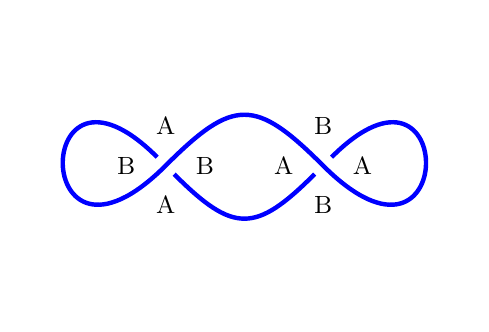
\begin{tikzpicture}
   \node (a) at (-1,0) {};
   \node (b) at ( 1,0) {};
   \draw 
     (a.center) .. controls (a.8  north east) and (b.8  north west) ..
     (b.center) .. controls (b.16 south east) and (b.16 north east) ..
     (b)        .. controls (b.8  south west) and (a.8  south east) ..
     (a)        .. controls (a.16 north west) and (a.16 south west) ..
     (a.center);
   \draw[black] (-1.0, 0.5) node{\small A};
   \draw[black] (-1.0,-0.5) node{\small A};
   \draw[black] (-1.5, 0.0) node{\small B};
   \draw[black] (-0.5, 0.0) node{\small B};
   \draw[black] ( 1.0, 0.5) node{\small B};
   \draw[black] ( 1.0,-0.5) node{\small B};
   \draw[black] ( 1.5, 0.0) node{\small A};
   \draw[black] ( 0.5, 0.0) node{\small A};
  \end{tikzpicture}
 \end{center}

\bigskip

\begin{center}
 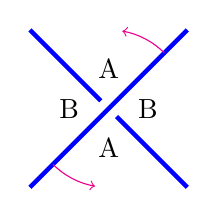
\begin{tikzpicture}
  \draw (-1.0,-1.0) -- ( 1.0, 1.0);
  \draw ( 1.0,-1.0) -- ( 0.1,-0.1);
  \draw (-0.1, 0.1) -- (-1.0, 1.0);
  \draw[thin,magenta,->] (0,0) ( 45:1) arc( 45: 80:1); 
  \draw[thin,magenta,->] (0,0) (225:1) arc(225:260:1); 
  \draw[black] ( 0.0, 0.5) node {A};
  \draw[black] ( 0.0,-0.5) node {A};
  \draw[black] ( 0.5, 0.0) node {B};
  \draw[black] (-0.5, 0.0) node {B};   
 \end{tikzpicture}
\end{center}

\begin{center}
 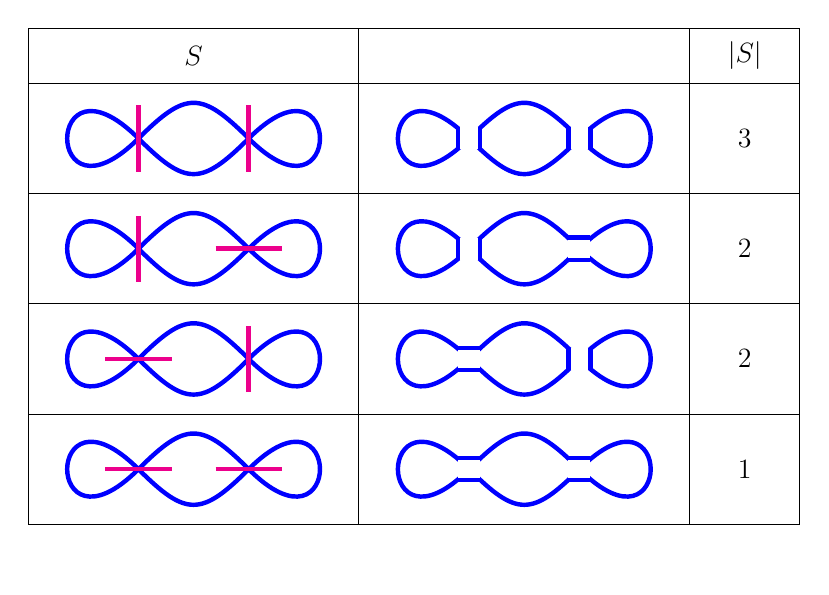
\begin{tikzpicture}[scale=0.7]
  \draw[thin,black] (-3.0, 2) -- (11.0, 2);
  \draw[thin,black] (-3.0, 1) -- (11.0, 1);
  \draw[thin,black] (-3.0,-1) -- (11.0,-1);
  \draw[thin,black] (-3.0,-3) -- (11.0,-3);
  \draw[thin,black] (-3.0,-5) -- (11.0,-5);
  \draw[thin,black] (-3.0,-7) -- (11.0,-7);
  \draw[thin,black] (-3.0, 2) -- (-3.0,-7);
  \draw[thin,black] ( 3.0, 2) -- ( 3.0,-7);
  \draw[thin,black] ( 9.0, 2) -- ( 9.0,-7);
  \draw[thin,black] (11.0, 2) -- (11.0,-7);
  \draw[black] ( 0,1.5) node {\Large $S$};
  \draw[black] (10,1.5) node {\Large $|S|$};
  \draw[black] (10, 0) node {\Large $3$};
  \draw[black] (10,-2) node {\Large $2$};
  \draw[black] (10,-4) node {\Large $2$};
  \draw[black] (10,-6) node {\Large $1$};

  \begin{scope}[scale=2]
   \node (a) at (-0.5,0) {};
   \node (b) at ( 0.5,0) {};
   \draw 
    (a.center) .. controls (a.4 north east) and (b.4 north west) ..
    (b.center) .. controls (b.8 south east) and (b.8 north east) ..
    (b.center) .. controls (b.4 south west) and (a.4 south east) ..
    (a.center) .. controls (a.8 north west) and (a.8 south west) ..
    (a.center);
   \draw[magenta] (-0.5,-0.3) -- (-0.5,0.3);
   \draw[magenta] ( 0.5,-0.3) -- ( 0.5,0.3);
  \end{scope}
  \begin{scope}[scale=2,yshift=-1cm]
   \node (a) at (-0.5,0) {};
   \node (b) at ( 0.5,0) {};
   \draw 
    (a.center) .. controls (a.4 north east) and (b.4 north west) ..
    (b.center) .. controls (b.8 south east) and (b.8 north east) ..
    (b.center) .. controls (b.4 south west) and (a.4 south east) ..
    (a.center) .. controls (a.8 north west) and (a.8 south west) ..
    (a.center);
   \draw[magenta] (-0.5,-0.3) -- (-0.5,0.3);
   \draw[magenta] ( 0.2, 0.0) -- ( 0.8,0.0);
  \end{scope}
  \begin{scope}[scale=2,yshift=-2cm]
   \node (a) at (-0.5,0) {};
   \node (b) at ( 0.5,0) {};
   \draw 
    (a.center) .. controls (a.4 north east) and (b.4 north west) ..
    (b.center) .. controls (b.8 south east) and (b.8 north east) ..
    (b.center) .. controls (b.4 south west) and (a.4 south east) ..
    (a.center) .. controls (a.8 north west) and (a.8 south west) ..
    (a.center);
   \draw[magenta] (-0.8, 0.0) -- (-0.2,0.0);
   \draw[magenta] ( 0.5,-0.3) -- ( 0.5,0.3);
  \end{scope}
  \begin{scope}[scale=2,yshift=-3cm]
   \node (a) at (-0.5,0) {};
   \node (b) at ( 0.5,0) {};
   \draw 
    (a.center) .. controls (a.4 north east) and (b.4 north west) ..
    (b.center) .. controls (b.8 south east) and (b.8 north east) ..
    (b.center) .. controls (b.4 south west) and (a.4 south east) ..
    (a.center) .. controls (a.8 north west) and (a.8 south west) ..
    (a.center);
   \draw[magenta] (-0.8, 0.0) -- (-0.2,0.0);
   \draw[magenta] ( 0.2, 0.0) -- ( 0.8,0.0);
  \end{scope}
  \begin{scope}[xshift=6cm,scale=2]
   \node (a) at (-0.5,0) {};
   \node (b) at ( 0.5,0) {};
   \draw 
    (a.center) .. controls (a.4 north east) and (b.4 north west) ..
    (b.center) .. controls (b.8 south east) and (b.8 north east) ..
    (b.center) .. controls (b.4 south west) and (a.4 south east) ..
    (a.center) .. controls (a.8 north west) and (a.8 south west) ..
    (a.center);
   \begin{scope}[xshift=-0.5cm] 
    \fill[white] (-0.1,-0.1) rectangle (0.1,0.1);
    \draw (-0.1,-0.1) -- (-0.1,0.1);
    \draw ( 0.1,-0.1) -- ( 0.1,0.1);
   \end{scope}
   \begin{scope}[xshift= 0.5cm] 
    \fill[white] (-0.1,-0.1) rectangle (0.1,0.1);
    \draw (-0.1,-0.1) -- (-0.1,0.1);
    \draw ( 0.1,-0.1) -- ( 0.1,0.1);
   \end{scope}
  \end{scope}
  \begin{scope}[xshift=6cm,scale=2,yshift=-1cm]
   \node (a) at (-0.5,0) {};
   \node (b) at ( 0.5,0) {};
   \draw 
    (a.center) .. controls (a.4 north east) and (b.4 north west) ..
    (b.center) .. controls (b.8 south east) and (b.8 north east) ..
    (b.center) .. controls (b.4 south west) and (a.4 south east) ..
    (a.center) .. controls (a.8 north west) and (a.8 south west) ..
    (a.center);
   \begin{scope}[xshift=-0.5cm] 
    \fill[white] (-0.1,-0.1) rectangle (0.1,0.1);
    \draw (-0.1,-0.1) -- (-0.1,0.1);
    \draw ( 0.1,-0.1) -- ( 0.1,0.1);
   \end{scope}
   \begin{scope}[xshift= 0.5cm] 
    \fill[white] (-0.1,-0.1) rectangle (0.1,0.1);
    \draw (-0.1,-0.1) -- ( 0.1,-0.1);
    \draw (-0.1, 0.1) -- ( 0.1, 0.1);
   \end{scope}
  \end{scope}
  \begin{scope}[xshift=6cm,scale=2,yshift=-2cm]
   \node (a) at (-0.5,0) {};
   \node (b) at ( 0.5,0) {};
   \draw 
    (a.center) .. controls (a.4 north east) and (b.4 north west) ..
    (b.center) .. controls (b.8 south east) and (b.8 north east) ..
    (b.center) .. controls (b.4 south west) and (a.4 south east) ..
    (a.center) .. controls (a.8 north west) and (a.8 south west) ..
    (a.center);
   \begin{scope}[xshift=-0.5cm] 
    \fill[white] (-0.1,-0.1) rectangle (0.1,0.1);
    \draw (-0.1,-0.1) -- ( 0.1,-0.1);
    \draw (-0.1, 0.1) -- ( 0.1, 0.1);
   \end{scope}
   \begin{scope}[xshift= 0.5cm] 
    \fill[white] (-0.1,-0.1) rectangle (0.1,0.1);
    \draw (-0.1,-0.1) -- (-0.1,0.1);
    \draw ( 0.1,-0.1) -- ( 0.1,0.1);
   \end{scope}
  \end{scope}
  \begin{scope}[xshift=6cm,scale=2,yshift=-3cm]
   \node (a) at (-0.5,0) {};
   \node (b) at ( 0.5,0) {};
   \draw 
    (a.center) .. controls (a.4 north east) and (b.4 north west) ..
    (b.center) .. controls (b.8 south east) and (b.8 north east) ..
    (b.center) .. controls (b.4 south west) and (a.4 south east) ..
    (a.center) .. controls (a.8 north west) and (a.8 south west) ..
    (a.center);
   \begin{scope}[xshift=-0.5cm] 
    \fill[white] (-0.1,-0.1) rectangle (0.1,0.1);
    \draw (-0.1,-0.1) -- ( 0.1,-0.1);
    \draw (-0.1, 0.1) -- ( 0.1, 0.1);
   \end{scope}
   \begin{scope}[xshift= 0.5cm] 
    \fill[white] (-0.1,-0.1) rectangle (0.1,0.1);
    \draw (-0.1,-0.1) -- ( 0.1,-0.1);
    \draw (-0.1, 0.1) -- ( 0.1, 0.1);
   \end{scope}
  \end{scope}
 \end{tikzpicture}
\end{center}

\begin{center}
 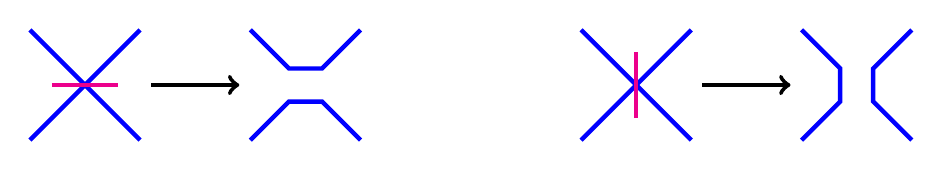
\begin{tikzpicture}[scale=0.7]
  \begin{scope}
   \draw (-1,-1) -- (1,1);
   \draw (-1,1) -- (1,-1);
   \draw[magenta] (-0.6,0) -- (0.6,0);
   \draw[->,black] (1.2,0) -- (2.8,0);
  \end{scope}
  \begin{scope}[xshift=4cm]
   \draw (-1,-1) -- (-0.3,-0.3) -- (0.3,-0.3) -- (1,-1);
   \draw (-1, 1) -- (-0.3, 0.3) -- (0.3, 0.3) -- (1, 1);
  \end{scope}
  \begin{scope}[xshift=10cm]
   \draw (-1,-1) -- (1,1);
   \draw (-1,1) -- (1,-1);
   \draw[magenta] (0,-0.6) -- (0,0.6);
   \draw[->,black] (1.2,0) -- (2.8,0);
  \end{scope}
  \begin{scope}[xshift=14cm]
   \draw (-1,-1) -- (-0.3,-0.3) -- (-0.3,0.3) -- (-1,1);
   \draw ( 1,-1) -- ( 0.3,-0.3) -- (0.3, 0.3) -- (1, 1);
  \end{scope}
 \end{tikzpicture}
\end{center}

\begin{center}
 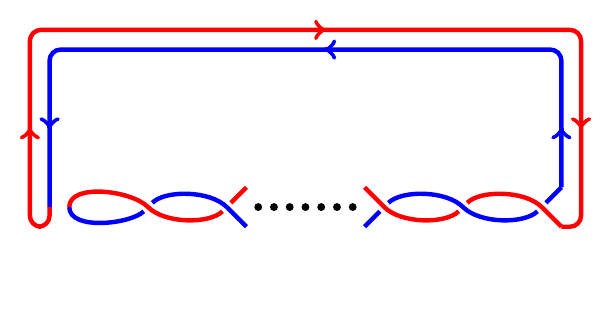
\begin{tikzpicture}[scale=0.5]
  \node (a) at (-6,0) {};
  \node (b) at (-4,0) {};
  \node (c) at (-2,0) {};
  \node (d) at ( 2,0) {};
  \node (e) at ( 4,0) {};
  \node (f) at ( 6,0) {};
  \draw 
   (1.5,-0.5) .. controls (d.4 south west) .. 
   (d)        .. controls (d.4 north east) and (e.4 north west) ..
   (e.center) .. controls (e.4 south east) and (f.4 south west) ..
   (f)        .. controls (f.4 north east) .. (6.5,0.5);
  \draw[rounded corners] (6.5,0.5) -- (6.5,4) -- (-6.5,4) -- (-6.5,0.0);
  \draw
   (a.center) .. controls (a.4 south) and (b.4 south west) ..
   (b)        .. controls (b.4 north east) and (c.4 north west) ..
   (c.center) .. controls (c.4 south east) .. (-1.5,-0.5);
  \draw[red] 
   (1.5, 0.5) .. controls (d.4 north west) .. 
   (d.center) .. controls (d.4 south east) and (e.4 south west) ..
   (e)        .. controls (e.4 north east) and (f.4 north west) ..
   (f.center) .. controls (f.4 south east) .. (6.5,-0.5);
  \draw[red,rounded corners]
   (6.5,-0.5) -- (7,-0.5) -- (7,4.5) -- (-7,4.5) -- (-7,-0.5) -- (-6.5,-0.5) -- (-6.5,0);
  \draw[red]
   (a.center) .. controls (a.4 north) and (b.4 north west) ..
   (b.center) .. controls (b.4 south east) and (c.4 south west) ..
   (c) .. controls (c.4 north east) .. (-1.5, 0.5);
  \draw[red, ->] (-7.0,2.0) -- +(0, 0.01);
  \draw[red, ->] ( 0.5,4.5) -- +( 0.01,0);
  \draw[red, ->] ( 7.0,2.0) -- +(0,-0.01);
  \draw[blue,->] (-6.5,2.0) -- +(0,-0.01);
  \draw[blue,->] (0.5,4.0) -- +(-0.01,0);
  \draw[blue,->] ( 6.5,2.0) -- +(0, 0.01);
  \fill[black] (-1.2,0) circle(0.1);
  \fill[black] (-0.8,0) circle(0.1);
  \fill[black] (-0.4,0) circle(0.1);
  \fill[black] ( 0.0,0) circle(0.1);
  \fill[black] ( 0.4,0) circle(0.1);
  \fill[black] ( 0.8,0) circle(0.1);
  \fill[black] ( 1.2,0) circle(0.1);
  \draw[white] (-6,-2) -- (6,-2);
 \end{tikzpicture}
\end{center}

\begin{center}
 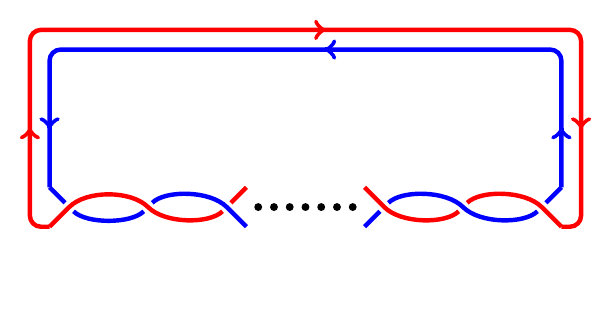
\begin{tikzpicture}[scale=0.5]
  \node (a) at (-6,0) {};
  \node (b) at (-4,0) {};
  \node (c) at (-2,0) {};
  \node (d) at ( 2,0) {};
  \node (e) at ( 4,0) {};
  \node (f) at ( 6,0) {};
  \draw 
   (1.5,-0.5) .. controls (d.4 south west) .. 
   (d)        .. controls (d.4 north east) and (e.4 north west) ..
   (e.center) .. controls (e.4 south east) and (f.4 south west) ..
   (f)        .. controls (f.4 north east) .. (6.5,0.5);
  \draw[rounded corners] (6.5,0.5) -- (6.5,4) -- (-6.5,4) -- (-6.5,0.5);
  \draw
   (-6.5,0.5) .. controls (a.4 north west) ..
   (a)        .. controls (a.4 south east) and (b.4 south west) ..
   (b)        .. controls (b.4 north east) and (c.4 north west) ..
   (c.center) .. controls (c.4 south east) .. (-1.5,-0.5);
  \draw[red] 
   (1.5, 0.5) .. controls (d.4 north west) .. 
   (d.center) .. controls (d.4 south east) and (e.4 south west) ..
   (e)        .. controls (e.4 north east) and (f.4 north west) ..
   (f.center) .. controls (f.4 south east) .. (6.5,-0.5);
  \draw[red,rounded corners] (6.5,-0.5) -- (7,-0.5) -- (7,4.5) -- (-7,4.5) -- (-7,-0.5) -- (-6.5,-0.5);
  \draw[red]
   (-6.5,-0.5) .. controls (a.4 south west) ..
   (a.center) .. controls (a.4 north east) and (b.4 north west) ..
   (b.center) .. controls (b.4 south east) and (c.4 south west) ..
   (c) .. controls (c.4 north east) .. (-1.5, 0.5);
  \draw[red, ->] (-7.0,2.0) -- +(0, 0.01);
  \draw[red, ->] ( 0.5,4.5) -- +( 0.01,0);
  \draw[red, ->] ( 7.0,2.0) -- +(0,-0.01);
  \draw[blue,->] (-6.5,2.0) -- +(0,-0.01);
  \draw[blue,->] (0.5,4.0) -- +(-0.01,0);
  \draw[blue,->] ( 6.5,2.0) -- +(0, 0.01);
  \fill[black] (-1.2,0) circle(0.1);
  \fill[black] (-0.8,0) circle(0.1);
  \fill[black] (-0.4,0) circle(0.1);
  \fill[black] ( 0.0,0) circle(0.1);
  \fill[black] ( 0.4,0) circle(0.1);
  \fill[black] ( 0.8,0) circle(0.1);
  \fill[black] ( 1.2,0) circle(0.1);
  \draw[white] (-6,-2) -- (6,-2);
 \end{tikzpicture}
\end{center}


\begin{center}
 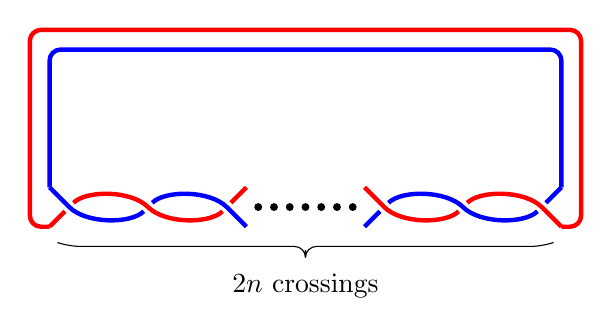
\begin{tikzpicture}[scale=0.5]
  \node (a) at (-6,0) {};
  \node (b) at (-4,0) {};
  \node (c) at (-2,0) {};
  \node (d) at ( 2,0) {};
  \node (e) at ( 4,0) {};
  \node (f) at ( 6,0) {};
  \draw 
   (1.5,-0.5) .. controls (d.4 south west) .. 
   (d)        .. controls (d.4 north east) and (e.4 north west) ..
   (e.center) .. controls (e.4 south east) and (f.4 south west) ..
   (f)        .. controls (f.4 north east) .. (6.5,0.5);
  \draw[rounded corners] (6.5,0.5) -- (6.5,4) -- (-6.5,4) -- (-6.5,0.5);
  \draw
   (-6.5,0.5) .. controls (a.4 north west) ..
   (a.center) .. controls (a.4 south east) and (b.4 south west) ..
   (b) .. controls (b.4 north east) and (c.4 north west) ..
   (c.center) .. controls (c.4 south east) .. (-1.5,-0.5);
  \draw[red] 
   (1.5, 0.5) .. controls (d.4 north west) .. 
   (d.center) .. controls (d.4 south east) and (e.4 south west) ..
   (e)        .. controls (e.4 north east) and (f.4 north west) ..
   (f.center) .. controls (f.4 south east) .. (6.5,-0.5);
  \draw[red,rounded corners] (6.5,-0.5) -- (7,-0.5) -- (7,4.5) -- (-7,4.5) -- (-7,-0.5) -- (-6.5,-0.5);
  \draw[red]
   (-6.5,-0.5) .. controls (a.4 south west) ..
   (a) .. controls (a.4 north east) and (b.4 north west) ..
   (b.center) .. controls (b.4 south east) and (c.4 south west) ..
   (c) .. controls (c.4 north east) .. (-1.5, 0.5);
  \fill[black] (-1.2,0) circle(0.1);
  \fill[black] (-0.8,0) circle(0.1);
  \fill[black] (-0.4,0) circle(0.1);
  \fill[black] ( 0.0,0) circle(0.1);
  \fill[black] ( 0.4,0) circle(0.1);
  \fill[black] ( 0.8,0) circle(0.1);
  \fill[black] ( 1.2,0) circle(0.1);
  \draw[thin,black,rounded corners]
   (-6.3,-0.9) -- (-6,-1.0) -- (0,-1.0) -- (0,-1.1);
  \draw[thin,black,rounded corners]
   ( 6.3,-0.9) -- ( 6,-1.0) -- (0,-1.0) -- (0,-1.1);
  \begin{scope}[scale=2]
   \draw[black] (0,-1) node{$2n$ crossings};
  \end{scope}
 \end{tikzpicture}
\end{center}

\begin{center}
 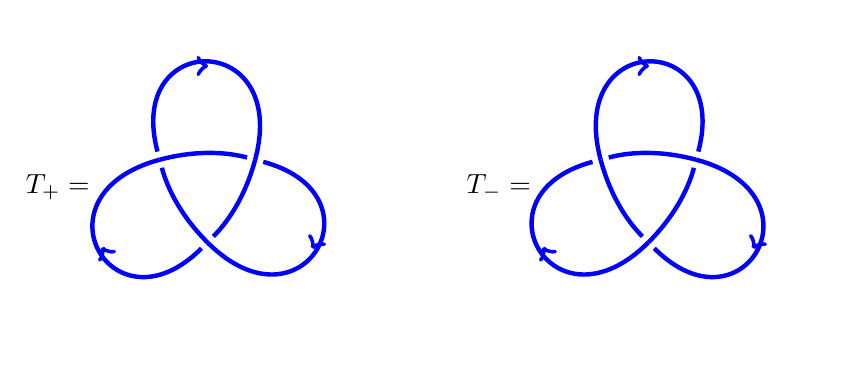
\begin{tikzpicture}
  \begin{scope}[scale=0.7]
   \begin{scope}[rotate=  0] \node (a) at (0,-1) {}; \end{scope}
   \begin{scope}[rotate=120] \node (b) at (0,-1) {}; \end{scope}
   \begin{scope}[rotate=240] \node (c) at (0,-1) {}; \end{scope}
   \draw (a.center) .. controls (a.4 north west) and (c.4 north east) .. (c);
   \draw (b.center) .. controls (b.4 north west) and (a.4 north east) .. (a);
   \draw (c.center) .. controls (c.4 north west) and (b.4 north east) .. (b);
   \draw (a) .. controls (a.16 south west) and (c.16 south east) .. (c.center);
   \draw (b) .. controls (b.16 south west) and (a.16 south east) .. (a.center);
   \draw (c) .. controls (c.16 south west) and (b.16 south east) .. (b.center);
   \draw[->] ( 90:2.2) -- +(  0:0.01);
   \draw[->] (210:2.2) -- +(120:0.01);
   \draw[->] (330:2.2) -- +(240:0.01);
  \end{scope}
  \draw[black] (-1.9,0) node {$T_+=$};
  \begin{scope}[scale=0.7,xshift=8cm]
   \begin{scope}[rotate=  0] \node (a) at (0,-1) {}; \end{scope}
   \begin{scope}[rotate=120] \node (b) at (0,-1) {}; \end{scope}
   \begin{scope}[rotate=240] \node (c) at (0,-1) {}; \end{scope}
   \draw (a) .. controls (a.4 north west) and (c.4 north east) .. (c.center);
   \draw (b) .. controls (b.4 north west) and (a.4 north east) .. (a.center);
   \draw (c) .. controls (c.4 north west) and (b.4 north east) .. (b.center);
   \draw (a.center) .. controls (a.16 south west) and (c.16 south east) .. (c);
   \draw (b.center) .. controls (b.16 south west) and (a.16 south east) .. (a);
   \draw (c.center) .. controls (c.16 south west) and (b.16 south east) .. (b);
   \draw[->] ( 90:2.2) -- +(  0:0.01);
   \draw[->] (210:2.2) -- +(120:0.01);
   \draw[->] (330:2.2) -- +(240:0.01);
  \end{scope}
  \draw[black] ( 3.7,0) node {$T_-=$};
 \end{tikzpicture}
\end{center}

\begin{center}
 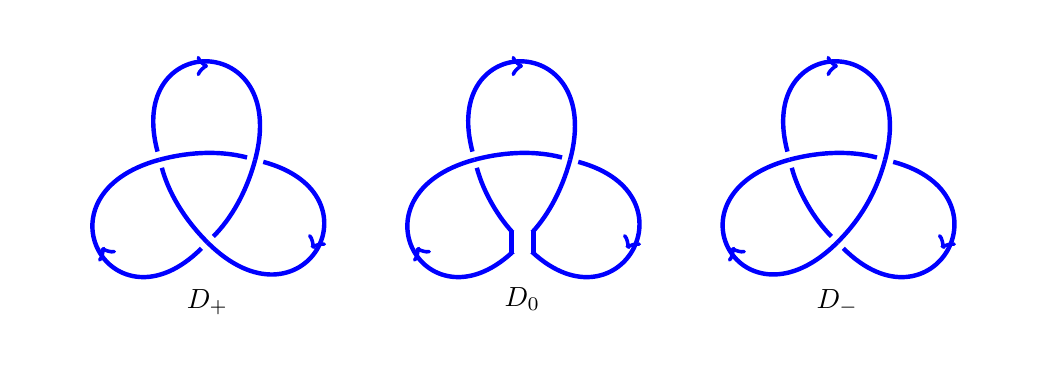
\begin{tikzpicture}
  \begin{scope}[scale=0.7]
   \begin{scope}[rotate=  0] \node (a) at (0,-1) {}; \end{scope}
   \begin{scope}[rotate=120] \node (b) at (0,-1) {}; \end{scope}
   \begin{scope}[rotate=240] \node (c) at (0,-1) {}; \end{scope}
   \draw (a.center) .. controls (a.4 north west) and (c.4 north east) .. (c);
   \draw (b.center) .. controls (b.4 north west) and (a.4 north east) .. (a);
   \draw (c.center) .. controls (c.4 north west) and (b.4 north east) .. (b);
   \draw (a)        .. controls (a.16 south west) and (c.16 south east) .. (c.center);
   \draw (b)        .. controls (b.16 south west) and (a.16 south east) .. (a.center);
   \draw (c)        .. controls (c.16 south west) and (b.16 south east) .. (b.center);
   \draw[->] ( 90:2.2) -- +(  0:0.01);
   \draw[->] (210:2.2) -- +(120:0.01);
   \draw[->] (330:2.2) -- +(240:0.01);
  \end{scope}
  \begin{scope}[xshift=4cm,scale=0.7]
   \begin{scope}[rotate=  0] \node (a) at (0,-1) {}; \end{scope}
   \begin{scope}[rotate=120] \node (b) at (0,-1) {}; \end{scope}
   \begin{scope}[rotate=240] \node (c) at (0,-1) {}; \end{scope}
   \draw (a)        .. controls (a.4 north west) and (c.4 north east) .. (c);
   \draw (b.center) .. controls (b.4 north west) and (a.4 north east) .. (a);
   \draw (c.center) .. controls (c.4 north west) and (b.4 north east) .. (b);
   \draw (a)        .. controls (a.16 south west) and (c.16 south east) .. (c.center);
   \draw (b)        .. controls (b.16 south west) and (a.16 south east) .. (a);
   \draw (c)        .. controls (c.16 south west) and (b.16 south east) .. (b.center);
   \draw[->] ( 90:2.2) -- +(  0:0.01);
   \draw[->] (210:2.2) -- +(120:0.01);
   \draw[->] (330:2.2) -- +(240:0.01);
   \fill[white] (-0.2,-1.2) rectangle (0.2,-0.8);
   \draw (-0.2,-1.2) -- (-0.2,-0.8);
   \draw ( 0.2,-1.2) -- ( 0.2,-0.8);
  \end{scope}
  \begin{scope}[xshift=8cm,scale=0.7]
   \begin{scope}[rotate=  0] \node (a) at (0,-1) {}; \end{scope}
   \begin{scope}[rotate=120] \node (b) at (0,-1) {}; \end{scope}
   \begin{scope}[rotate=240] \node (c) at (0,-1) {}; \end{scope}
   \draw (a)        .. controls (a.4 north west) and (c.4 north east) .. (c);
   \draw (b.center) .. controls (b.4 north west) and (a.4 north east) .. (a.center);
   \draw (c.center) .. controls (c.4 north west) and (b.4 north east) .. (b);
   \draw (a.center) .. controls (a.16 south west) and (c.16 south east) .. (c.center);
   \draw (b)        .. controls (b.16 south west) and (a.16 south east) .. (a);
   \draw (c)        .. controls (c.16 south west) and (b.16 south east) .. (b.center);
   \draw[->] ( 90:2.2) -- +(  0:0.01);
   \draw[->] (210:2.2) -- +(120:0.01);
   \draw[->] (330:2.2) -- +(240:0.01);
  \end{scope}
  \draw[black] (0,-1) node[anchor=north] {$D_+$};
  \draw[black] (4,-1) node[anchor=north] {$D_0$};
  \draw[black] (8,-1) node[anchor=north] {$D_-$};
  \draw[white] (0,-1.2) -- (8,-1.2);
 \end{tikzpicture}
\end{center}

\begin{center}
 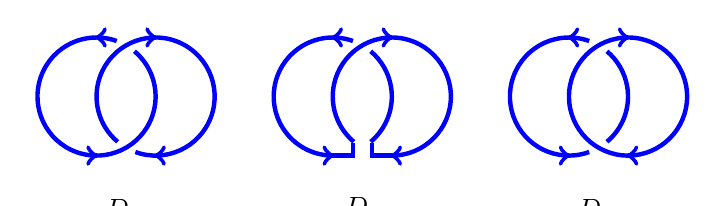
\begin{tikzpicture}[scale=1.5]
  \begin{scope}
   \draw (-0.25,0) +( 70: 0.5) arc( 70:410: 0.5);
   \draw ( 0.25,0) +( 70:-0.5) arc( 70:410:-0.5);
   \draw[->] (-0.25,-0.50) -- +( 0.01,0);
   \draw[->] ( 0.25,-0.50) -- +(-0.01,0);
   \draw[->] (-0.25, 0.50) -- +(-0.01,0);
   \draw[->] ( 0.25, 0.50) -- +( 0.01,0);
   \begin{scope}[scale=0.67]
    \draw[black] (0,-1) node[anchor=north] {$D_+$}; 
   \end{scope}
  \end{scope}
  \begin{scope}[xshift=2cm]
   \draw (-0.25,0) +( 70: 0.5) arc( 70:270: 0.5);
   \draw (-0.25,0) +(-50: 0.5) arc(-50: 50: 0.5);
   \draw ( 0.25,0) +(-90: 0.5) arc(-90:230: 0.5);
   \draw (-0.25,-0.50) -- (-0.08,-0.50) -- (-0.08,-0.39);
   \draw ( 0.25,-0.50) -- ( 0.08,-0.50) -- ( 0.08,-0.39);
   \draw[->] (-0.25,-0.50) -- +( 0.01,0);
   \draw[->] ( 0.25,-0.50) -- +(-0.01,0);
   \draw[->] (-0.25, 0.50) -- +(-0.01,0);
   \draw[->] ( 0.25, 0.50) -- +( 0.01,0);
   \begin{scope}[scale=0.67]
    \draw[black] (0,-1) node[anchor=north] {$D_0$}; 
   \end{scope}
  \end{scope}
  \begin{scope}[xshift=4cm]
   \draw (-0.25,0) +(-50: 0.5) arc(-50: 50: 0.5);
   \draw (-0.25,0) +( 70: 0.5) arc( 70:290: 0.5);
   \draw ( 0.25,0) circle(0.5);
   \draw[->] (-0.25,-0.50) -- +( 0.01,0);
   \draw[->] ( 0.25,-0.50) -- +(-0.01,0);
   \draw[->] (-0.25, 0.50) -- +(-0.01,0);
   \draw[->] ( 0.25, 0.50) -- +( 0.01,0);
   \begin{scope}[scale=0.67]
    \draw[black] (0,-1) node[anchor=north] {$D_-$}; 
   \end{scope}
  \end{scope}
 \end{tikzpicture}
\end{center}

\begin{center}
 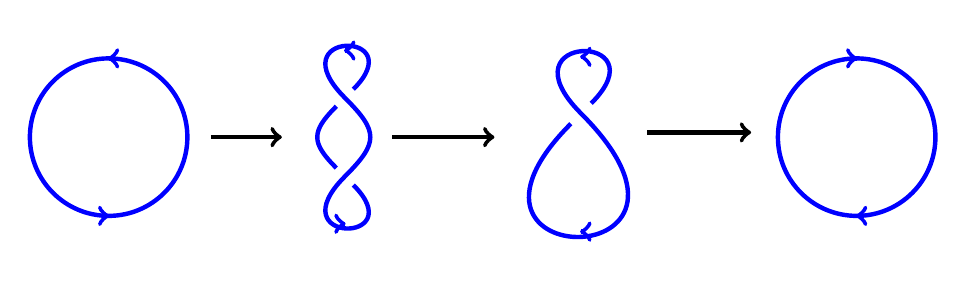
\begin{tikzpicture}
  \begin{scope}
   \draw(0,0) circle(1);
   \draw[->] (0, 1) -- +(-0.01,0);
   \draw[->] (0,-1) -- +( 0.01,0);
   \draw[black,->] (1.3,0) -- (2.2,0);
  \end{scope}
  \begin{scope}[xshift=3cm]
   \node (a) at (0, 0.5) {};
   \node (b) at (0,-0.5) {};
   \draw
    (a)        .. controls (a.8 north east) and (a.8 north west) ..
    (a.center) .. controls (a.4 south east) and (b.4 north east) ..
    (b.center) .. controls (b.8 south west) and (b.8 south east) ..
    (b)        .. controls (b.4 north west) and (a.4 south west) ..
    (a);
   \draw[->] (0, 1.1) -- +(-0.01,0);
   \draw[->] (0,-1.1) -- +( 0.01,0);
   \draw[black,->] (0.6,0,0) -- (1.9,0);
  \end{scope}
  \begin{scope}[xshift=6cm,yshift=-0.3cm,scale=1.2]
   \node (a) at (0, 0.5) {};
   \node (b) at (0,-0.5) {};
   \draw
    (a)        .. controls (a.8 north east) and (a.8 north west) ..
    (a.center) .. controls (a.16 south east) and (a.16 south west) ..
    (a);
   \draw[->] (0, 1.10) -- +(-0.01,0);
   \draw[->] (0,-0.75) -- +(-0.01,0);
   \draw[black,->] (0.7,0.3) -- (1.8,0.3);
  \end{scope}
  \begin{scope}[xshift=9.5cm]
   \draw(0,0) circle(1);
   \draw[->] (0, 1) -- +( 0.01,0);
   \draw[->] (0,-1) -- +(-0.01,0);
  \end{scope}
 \end{tikzpicture}
\end{center}

\begin{center}
 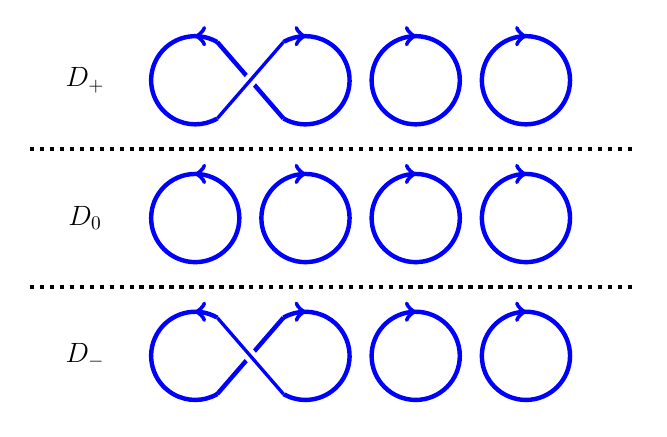
\begin{tikzpicture}[scale=0.7]
  \begin{scope}
   \draw (0,0) +(60: 0.8) arc(60:300: 0.8);
   \draw (2,0) +(60:-0.8) arc(60:300:-0.8);
   \draw (2,0) ++( 60:-0.8) -- ( 60:0.8);
   \draw[draw=white,double=blue ,ultra thick,double distance=1.2pt] (2,0) ++(300:-0.8) -- (300:0.8);
   \draw[->] (0,0.8) -- +(-0.01,0);
   \draw[->] (2,0.8) -- +( 0.01,0);
   \draw[->] (4,0.8) -- +( 0.01,0);
   \draw[->] (6,0.8) -- +( 0.01,0);
   \foreach \x in {4,6} {
    \draw (\x,0) circle (0.8);
   }
   \draw[black] (-2,0) node {\Large $D_+$};
  \end{scope}
  \draw[dotted,black] (-3,-1.25) -- (8,-1.25); 
  \begin{scope}[yshift=-2.5cm]
   \draw[->] (0,0.8) -- +(-0.01,0);
   \draw[->] (2,0.8) -- +( 0.01,0);
   \draw[->] (4,0.8) -- +( 0.01,0);
   \draw[->] (6,0.8) -- +( 0.01,0);
   \foreach \x in {0,2,4,6} {
    \draw (\x,0) circle (0.8);
   }
   \draw[black] (-2,0) node {\Large $D_0$};
  \end{scope}
  \draw[dotted,black] (-3,-3.75) -- (8,-3.75); 
  \begin{scope}[yshift=-5.0cm]
   \draw (0,0) +(60: 0.8) arc(60:300: 0.8);
   \draw (2,0) +(60:-0.8) arc(60:300:-0.8);
   \draw (2,0) ++(300:-0.8) -- (300:0.8);
   \draw[draw=white,double=blue ,ultra thick,double distance=1.2pt] (2,0) ++( 60:-0.8) -- ( 60:0.8);
   \draw[->] (0,0.8) -- +(-0.01,0);
   \draw[->] (2,0.8) -- +( 0.01,0);
   \draw[->] (4,0.8) -- +( 0.01,0);
   \draw[->] (6,0.8) -- +( 0.01,0);
   \foreach \x in {4,6} {
    \draw (\x,0) circle (0.8);
   }
   \draw[black] (-2,0) node {\Large $D_-$};
  \end{scope}
 \end{tikzpicture}
\end{center}

\begin{center}
 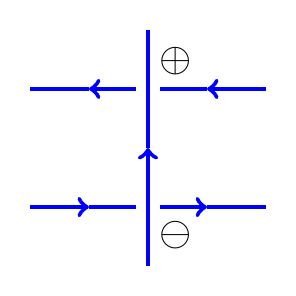
\begin{tikzpicture}[scale=1.5]
  \draw[->] (0,-1) -- (0,0);
  \draw (0,0) -- (0,1);
  \draw[->] (-1,-0.5) -- (-0.5,-0.5);
  \draw (-0.5,-0.5) -- (-0.1,-0.5);
  \draw[->] (0.1,-0.5) -- (0.5,-0.5);
  \draw (0.5,-0.5) -- (1,-0.5);
  \draw[->] (1,0.5) -- (0.5,0.5);
  \draw (0.5,0.5) -- (0.1,0.5);
  \draw[->] (-0.1,0.5) -- (-0.5,0.5);
  \draw (-0.5,0.5) -- (-1,0.5);
  \draw[black] (0, 0.5) node[anchor=south west] {$\oplus$};
  \draw[black] (0,-0.5) node[anchor=north west] {$\ominus$};
 \end{tikzpicture}
\end{center}


\begin{center}
 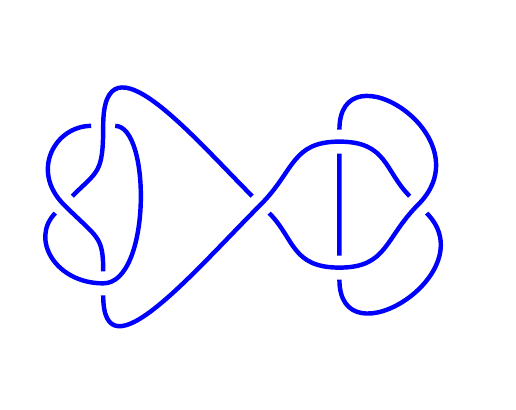
\begin{tikzpicture}
  \node (a) at (-2.0, 1.0) {};
  \node (b) at (-2.5, 0.0) {};
  \node (c) at (-2,-1.0) {};
  \node (d) at ( 0.0, 0.0) {};
  \node (e) at ( 1.0, 0.8) {};
  \node (f) at ( 1.0,-0.8) {};
  \node (g) at ( 2.0, 0.0) {};
  
  \draw
   (a)        .. controls (a.4 west) and (b.4 north west) ..
   (b.center) .. controls (b.4 south east) and (c.4 north) ..
   (c)        .. controls (c.8 south) and (d.8 south west) ..
   (d.center) .. controls (d.4 north east) and (e.4 west) ..
   (e.center) .. controls (e.4 east) and (g.4 north west) ..
   (g)        .. controls (g.8 south east) and (f.8 south) ..
   (f)        .. controls (f.4 north) and (e.4 south) ..
   (e)        .. controls (e.8 north) and (g.8 north east) ..
   (g.center) .. controls (g.4 south west) and (f.4 east) ..
   (f.center) .. controls (f.4 west) and (d.4 south east) ..
   (d)        .. controls (d.8 north west) and (a.8 north) ..
   (a.center) .. controls (a.4 south) and (b.4 north east) ..
   (b)        .. controls (b.4 south west) and (c.4 west) ..
   (c.center) .. controls (c.4 east) and (a.4 east) ..
   (a);
 \end{tikzpicture}
\end{center}

\begin{center}
 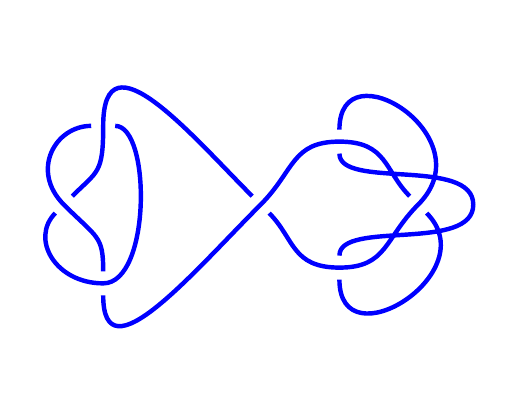
\begin{tikzpicture}
  \node (a) at (-2.0, 1.0) {};
  \node (b) at (-2.5, 0.0) {};
  \node (c) at (-2,-1.0) {};
  \node (d) at ( 0.0, 0.0) {};
  \node (e) at ( 1.0, 0.8) {};
  \node (f) at ( 1.0,-0.8) {};
  \node (g) at ( 2.0, 0.0) {};
  \node (h) at ( 2.7, 0.0) {};
  
  \draw
   (a)        .. controls (a.4 west) and (b.4 north west) ..
   (b.center) .. controls (b.4 south east) and (c.4 north) ..
   (c)        .. controls (c.8 south) and (d.8 south west) ..
   (d.center) .. controls (d.4 north east) and (e.4 west) ..
   (e.center) .. controls (e.4 east) and (g.4 north west) ..
   (g)        .. controls (g.8 south east) and (f.8 south) ..
   (f)        .. controls (f.4 north) and (h.4 south) ..
   (h.center) .. controls (h.4 north) and (e.4 south) .. 
   (e)        .. controls (e.8 north) and (g.8 north east) ..
   (g.center) .. controls (g.4 south west) and (f.4 east) ..
   (f.center) .. controls (f.4 west) and (d.4 south east) ..
   (d)        .. controls (d.8 north west) and (a.8 north) ..
   (a.center) .. controls (a.4 south) and (b.4 north east) ..
   (b)        .. controls (b.4 south west) and (c.4 west) ..
   (c.center) .. controls (c.4 east) and (a.4 east) ..
   (a);
 \end{tikzpicture}
\end{center}


\begin{center}
 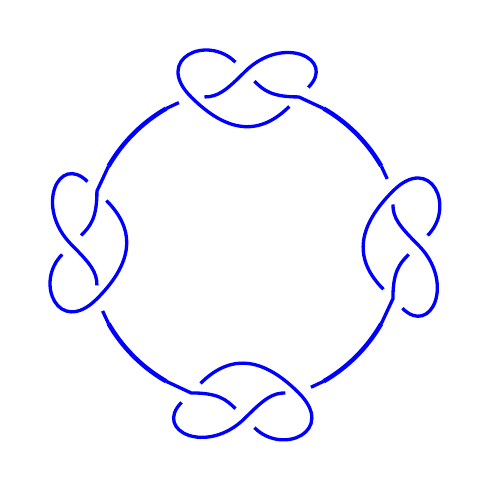
\begin{tikzpicture}[scale=0.4]
  \foreach \t in {0,90,180,270} {
   \begin{scope}[rotate=\t]
    \node[inner sep=8pt] (a) at ( 110:5.0) {};
    \node[inner sep=8pt] (b) at (  70:5.0) {};
    \node[inner sep=8pt] (c) at (  90:5.5) {};
    \draw[draw=white,double=blue ,ultra thick,double distance=1.2pt] (120:5) -- (a)
      .. controls (a.2 east) and (c.2 south west) .. (c.center)
      .. controls (c.4 north east) and (b.4 north east) .. (b)
      .. controls (b.4 south west) and (a.4 south east) .. (a.center)
      .. controls (a.4 north west) and (c.4 north west) .. (c)
      .. controls (c.2 south east) and (b.2 west) .. (b.center)
      -- (60:5);  
    \draw (0,0) (30:5) arc(30:60:5);
   \end{scope}
  }
 \end{tikzpicture}
\end{center}

\begin{center}
 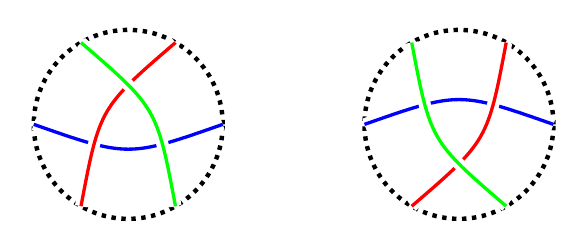
\begin{tikzpicture}[scale=0.6]
  \begin{scope}
   \draw[black,dotted] (0,0) circle(2);
   \draw[draw=white,double=blue ,ultra thick,double distance=1.2pt] (  0:2) .. controls (270:0.7) .. (180:2);
   \draw[draw=white,double=red  ,ultra thick,double distance=1.2pt] ( 60:2) .. controls (150:0.7) .. (240:2);
   \draw[draw=white,double=green,ultra thick,double distance=1.2pt] (120:2) .. controls ( 30:0.7) .. (300:2);
  \end{scope}
  \begin{scope}[xshift=7cm]
   \draw[black,dotted] (0,0) circle(2);
   \draw[draw=white,double=blue ,ultra thick,double distance=1.2pt] (  0:2) .. controls ( 90:0.7) .. (180:2);
   \draw[draw=white,double=red  ,ultra thick,double distance=1.2pt] ( 60:2) .. controls (330:0.7) .. (240:2);
   \draw[draw=white,double=green,ultra thick,double distance=1.2pt] (120:2) .. controls (210:0.7) .. (300:2);
  \end{scope}
 \end{tikzpicture}
\end{center}

\begin{center}
 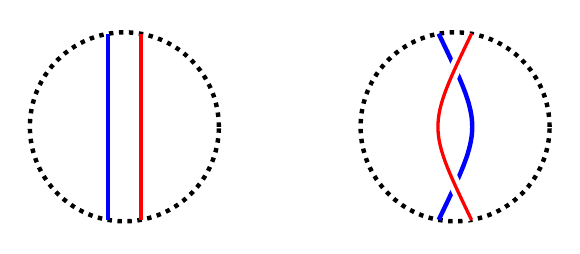
\begin{tikzpicture}[scale=0.6]
  \begin{scope}
   \draw[black,dotted] (0,0) circle(2);
   \draw[blue] (100:2) -- (260:2);
   \draw[red ] ( 80:2) -- (280:2);
  \end{scope}
  \begin{scope}[xshift=7cm]
   \draw[black,dotted] (0,0) circle(2);
   \draw[blue] (100:2) .. controls ( 0.6,0) .. (260:2); 
   \draw[draw=white,double=red,ultra thick,double distance=1.2pt] ( 80:2) .. controls (-0.6,0) .. (280:2);
  \end{scope}
 \end{tikzpicture}
\end{center}

\begin{center}
 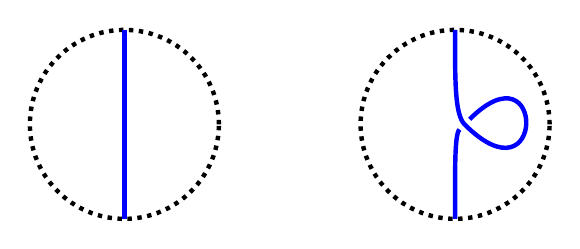
\begin{tikzpicture}[scale=0.6]
  \begin{scope}
   \draw[black,dotted] (0,0) circle(2);
   \draw (0,2) -- (0,-2);
  \end{scope}
  \begin{scope}[xshift=7cm]
   \node (a) at (0.2,0) {};
   \draw[black,dotted] (0,0) circle(2);
   \draw 
    (0,2) .. controls (0,1) and (a.2 north west) ..
    (a.center) .. controls (a.16 south east) and (a.16 north east) ..
    (a) .. controls (a.2 south west) and (0,-1) ..
    (0,-2);
  \end{scope}
 \end{tikzpicture}
\end{center}

% Reidemeister 1
\begin{center}
 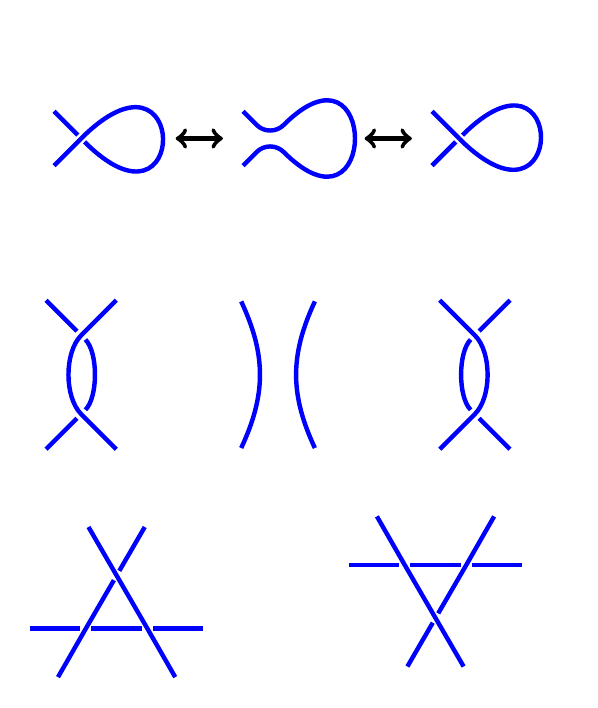
\begin{tikzpicture}
  \begin{scope}[scale=0.4]
   \node (a) {};
   \draw (a.center) .. controls (a.32 north east) and (a.32 south east) .. (a);
   \draw (a.center) -- (a.8 south west);
   \draw (a) -- (a.8 north west);
   \draw[double=none,black,<->] (3,0) -- ++(1.5,0);
   \begin{scope}[xshift=6cm]
    \node (b) {};
    \draw (b.8 north west) -- (b.4 north west) to[out=-45,in=-135] (b.4 north east) .. controls (b.32 north east) and (b.32 south east) .. (b.4 south east) to[out=135,in=45] (b.4 south west) -- (b.8 south west);
    \draw[double=none,black,<->] (3,0) -- ++(1.5,0);
   \end{scope}
   \begin{scope}[xshift=12cm]
    \node[rotate=90] (c) {};
    \draw (c.center) .. controls (c.32 south west) and (c.32 south east) .. (c);
    \draw (c.center) -- (c.8 north east);
    \draw (c) -- (c.8 north west);
   \end{scope}
  \end{scope}
  \begin{scope}[yshift=-3cm,scale=0.5]
   \begin{scope}
    \node (a) at (-1, 2) {};
    \node (b) at ( 1, 2) {};
    \node (c) at ( 0, 1) {};
    \node (d) at ( 0,-1) {};
    \node (e) at (-1,-2) {};
    \node (f) at ( 1,-2) {};
    \draw (a) .. controls (a.4 south east) and (c.4 north west) .. 
          (c) .. controls (c.4 south east) and (d.4 north east) ..
          (d) .. controls (d.4 south west) and (e.4 north east) .. (e);
    \draw (b) ..        controls (b.4 south west) and (c.4 north east) .. 
          (c.center) .. controls (c.4 south west) and (d.4 north west) ..
          (d.center) .. controls (d.4 south east) and (f.4 north west) .. (f);
   \end{scope}
   \begin{scope}[xshift=5cm]
    \node (a) at (-1, 2) {};
    \node (b) at ( 1, 2) {};
    \node (c) at ( 0, 1) {};
    \node (d) at ( 0,-1) {};
    \node (e) at (-1,-2) {};
    \node (f) at ( 1,-2) {};
    \draw (a) .. controls (-0.3, 0.5) and (-0.3,-0.5) .. (e);
    \draw (b) .. controls ( 0.3, 0.5) and ( 0.3,-0.5) .. (f);
   \end{scope}
   \begin{scope}[xshift=10cm]
    \node (a) at (-1, 2) {};
    \node (b) at ( 1, 2) {};
    \node (c) at ( 0, 1) {};
    \node (d) at ( 0,-1) {};
    \node (e) at (-1,-2) {};
    \node (f) at ( 1,-2) {};
    \draw (a)        .. controls (a.4 south east) and (c.4 north west) .. 
          (c.center) .. controls (c.4 south east) and (d.4 north east) ..
          (d.center) .. controls (d.4 south west) and (e.4 north east) .. (e);
    \draw (b) ..        controls (b.4 south west) and (c.4 north east) .. 
          (c) .. controls (c.4 south west) and (d.4 north west) ..
          (d) .. controls (d.4 south east) and (f.4 north west) .. (f);
   \end{scope}
  \end{scope}
  \begin{scope}[yshift=-6cm,scale=0.45]
   \begin{scope}[xshift=1cm]
    \node (a0) at ( 0.00, 1.00) {}; 
    \node (a1) at (-0.87,-0.50) {}; 
    \node (a2) at ( 0.87,-0.50) {}; 
    \node (b0) at ( 0.87, 2.50) {};
    \node (b1) at (-0.87, 2.50) {};
    \node (b2) at (-2.60,-0.50) {};
    \node (b3) at (-1.73,-2.00) {};
    \node (b4) at ( 1.73,-2.00) {};
    \node (b5) at ( 2.60,-0.50) {};

    \draw (b1) -- (a0.center) -- (a2.center) -- (b4);
    \draw (b0) -- (a0) -- (a1.center) -- (b3);
    \draw (b2) -- (a1) -- (a2) -- (b5);
   \end{scope}
   \begin{scope}[xshift=10cm,yshift=0.8cm]
    \node (a0) at ( 0.00,-1.00) {}; 
    \node (a1) at ( 0.87, 0.50) {}; 
    \node (a2) at (-0.87, 0.50) {}; 

    \node (b0) at ( 1.73, 2.00) {};
    \node (b1) at (-1.73, 2.00) {};
    \node (b2) at (-2.60, 0.50) {};
    \node (b3) at (-0.87,-2.50) {};
    \node (b4) at ( 0.87,-2.50) {};
    \node (b5) at ( 2.60, 0.50) {};

    \draw (b1) -- (a2.center) -- (a0.center) -- (b4);
    \draw (b0) -- (a1.center) -- (a0) -- (b3);
    \draw (b2) -- (a2) -- (a1) -- (b5);
   \end{scope}
  \end{scope}
 \end{tikzpicture}
\end{center}

\begin{center}
 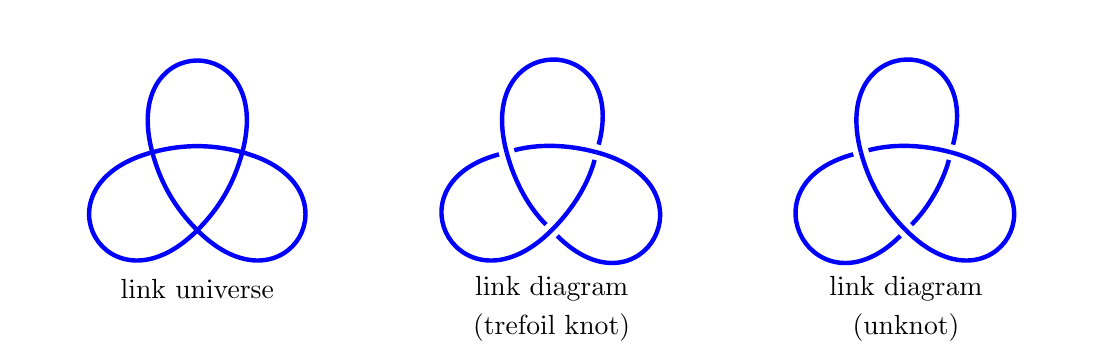
\begin{tikzpicture}
  \begin{scope}[scale=0.66]
   \begin{scope}[rotate=  0] \node (a) at (0,-1) {}; \end{scope}
   \begin{scope}[rotate=120] \node (b) at (0,-1) {}; \end{scope}
   \begin{scope}[rotate=240] \node (c) at (0,-1) {}; \end{scope}
   \draw (a.center) .. controls (a.4 north west) and (c.4 north east) .. (c.center);
   \draw (b.center) .. controls (b.4 north west) and (a.4 north east) .. (a.center);
   \draw (c.center) .. controls (c.4 north west) and (b.4 north east) .. (b.center);
   \draw (a.center) .. controls (a.16 south west) and (c.16 south east) .. (c.center);
   \draw (b.center) .. controls (b.16 south west) and (a.16 south east) .. (a.center);
   \draw (c.center) .. controls (c.16 south west) and (b.16 south east) .. (b.center);
  \end{scope}
  \begin{scope}[xshift=4.5cm,scale=0.66]
   \begin{scope}[rotate=  0] \node (a) at (0,-1) {}; \end{scope}
   \begin{scope}[rotate=120] \node (b) at (0,-1) {}; \end{scope}
   \begin{scope}[rotate=240] \node (c) at (0,-1) {}; \end{scope}
   \draw (a) .. controls (a.4 north west) and (c.4 north east) .. (c.center);
   \draw (b) .. controls (b.4 north west) and (a.4 north east) .. (a.center);
   \draw (c) .. controls (c.4 north west) and (b.4 north east) .. (b.center);
   \draw (a.center) .. controls (a.16 south west) and (c.16 south east) .. (c);
   \draw (b.center) .. controls (b.16 south west) and (a.16 south east) .. (a);
   \draw (c.center) .. controls (c.16 south west) and (b.16 south east) .. (b);
  \end{scope}
  \begin{scope}[xshift=9.0cm,scale=0.66]
   \begin{scope}[rotate=  0] \node (a) at (0,-1) {}; \end{scope}
   \begin{scope}[rotate=120] \node (b) at (0,-1) {}; \end{scope}
   \begin{scope}[rotate=240] \node (c) at (0,-1) {}; \end{scope}
   \draw (a.center) .. controls (a.4 north west) and (c.4 north east) .. (c.center);
   \draw (b)        .. controls (b.4 north west) and (a.4 north east) .. (a);
   \draw (c)        .. controls (c.4 north west) and (b.4 north east) .. (b.center);
   \draw (a)        .. controls (a.16 south west) and (c.16 south east) .. (c);
   \draw (b.center) .. controls (b.16 south west) and (a.16 south east) .. (a.center);
   \draw (c.center) .. controls (c.16 south west) and (b.16 south east) .. (b);
  \end{scope}
  \draw[black] (0.0,-1.4) node {link universe}; 
  \draw[black] (4.5,-1.4) node {link diagram}; 
  \draw[black] (4.5,-1.9) node {(trefoil knot)}; 
  \draw[black] (9.0,-1.4) node {link diagram}; 
  \draw[black] (9.0,-1.9) node {(unknot)}; 
 \end{tikzpicture}
\end{center}

\begin{center}
 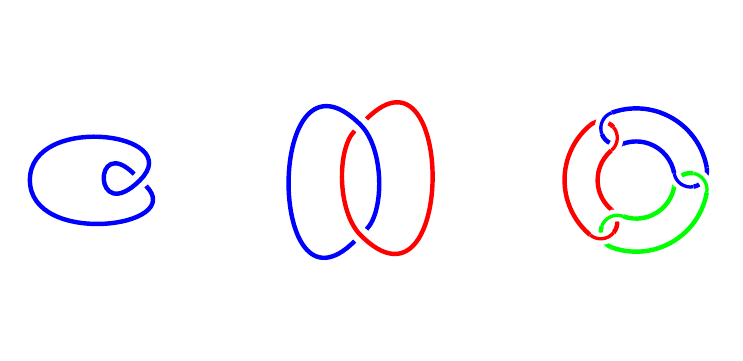
\begin{tikzpicture}[scale=0.7]
  \begin{scope}
   \node (a) at ( 1,0) {};
   \node (b) at (-1,0) {};
   \draw (a.center) .. controls (a.8 north east) and (b.8 north) ..
         (b.center) .. controls (b.8 south) and (a.8 south east) .. 
         (a) .. controls (a.8 north west) and (a.8 south west) .. (a.center);
  \end{scope}
  \begin{scope}[xshift=5cm]
   \node (a) at ( 0.00, 1.00) {};
   \node (b) at ( 0.00,-1.00) {};
   \draw[blue] (a.center) .. controls (a.4 south east) and (b.4 north east) ..
               (b) .. controls (b.16 south west) and (a.16 north west) .. (a.center);
   \draw[red]  (a) .. controls (a.4 south west) and (b.4 north west) ..
               (b.center) .. controls (b.16 south east) and (a.16 north east) .. (a);
  \end{scope}
  \begin{scope}[xshift=10cm]
   \begin{scope}[rotate=0]
    \draw[blue] (0,0) ( 10:1.3) arc( 10:110:1.3);
    \draw[blue] (0,0) ( 10:0.7) arc( 10:110:0.7);
    \draw[green] (350:1) +( 80:0.3) arc( 80:170:0.3);
    \draw[blue] ( 10:1) +(280:0.3) arc(280:370:0.3);
    \draw[draw=white,double=green,double distance=1.2pt] (350:1) +(350:0.3) arc(-10: 80:0.3);
    \draw[draw=white,double=blue,double distance=1.2pt] ( 10:1) +(190:0.3) arc(190:280:0.3);
   \end{scope}
   \begin{scope}[rotate=120]
    \draw[red] (0,0) ( 10:1.3) arc( 10:110:1.3);
    \draw[red] (0,0) ( 10:0.7) arc( 10:110:0.7);
    \draw[blue] (350:1) +( 80:0.3) arc( 80:170:0.3);
    \draw[red] ( 10:1) +(280:0.3) arc(280:370:0.3);
    \draw[draw=white,double=blue,double distance=1.2pt] (350:1) +(350:0.3) arc(-10: 80:0.3);
    \draw[draw=white,double=red,double distance=1.2pt] ( 10:1) +(190:0.3) arc(190:280:0.3);
   \end{scope}
   \begin{scope}[rotate=240]
    \draw[green] (0,0) ( 10:1.3) arc( 10:110:1.3);
    \draw[green] (0,0) ( 10:0.7) arc( 10:110:0.7);
    \draw[red] (350:1) +( 80:0.3) arc( 80:170:0.3);
    \draw[green] ( 10:1) +(280:0.3) arc(280:370:0.3);
    \draw[draw=white,double=red,double distance=1.2pt] (350:1) +(350:0.3) arc(-10: 80:0.3);
    \draw[draw=white,double=green,double distance=1.2pt] ( 10:1) +(190:0.3) arc(190:280:0.3);
   \end{scope}
  \end{scope}
 \end{tikzpicture}
\end{center}

\begin{center}
 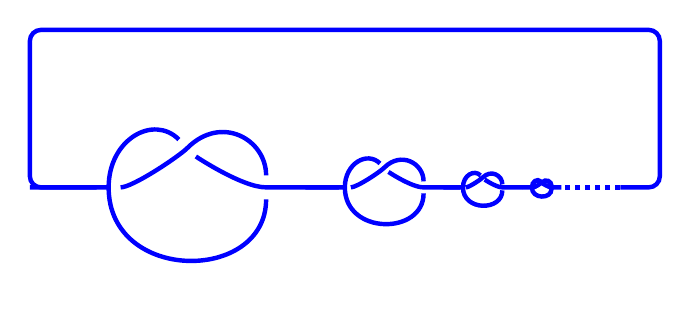
\begin{tikzpicture}
  \begin{scope}
   \node (a) at (-1.00, 0.00) {};
   \node (b) at ( 1.00, 0.00) {};
   \node (c) at ( 0.00, 0.50) {};
   \draw (-2,0) -- (a)
     .. controls (a.2 east) and (c.south west) .. (c.center)
     .. controls (c.4 north east) and (b.4 north) .. (b)
     .. controls (b.8 south) and (a.8 south) .. (a.center)
     .. controls (a.4 north) and (c.4 north west) .. (c)
     .. controls (c.south east) and (b.2 west) .. (b.center)
     -- (2,0);
  \end{scope}
  \begin{scope}[scale=0.5,xshift=5cm]
   \node (a) at (-1.00, 0.00) {};
   \node (b) at ( 1.00, 0.00) {};
   \node (c) at ( 0.00, 0.50) {};
   \draw (-2,0) -- (a)
     .. controls (a.2 east) and (c.south west) .. (c.center)
     .. controls (c.4 north east) and (b.4 north) .. (b)
     .. controls (b.8 south) and (a.8 south) .. (a.center)
     .. controls (a.4 north) and (c.4 north west) .. (c)
     .. controls (c.south east) and (b.2 west) .. (b.center)
     -- (2,0);
  \end{scope}
  \begin{scope}[scale=0.25,xshift=15cm]
   \node (a) at (-1.00, 0.00) {};
   \node (b) at ( 1.00, 0.00) {};
   \node (c) at ( 0.00, 0.50) {};
   \draw (-2,0) -- (a)
     .. controls (a.2 east) and (c.south west) .. (c.center)
     .. controls (c.4 north east) and (b.4 north) .. (b)
     .. controls (b.8 south) and (a.8 south) .. (a.center)
     .. controls (a.4 north) and (c.4 north west) .. (c)
     .. controls (c.south east) and (b.2 west) .. (b.center)
     -- (2,0);
  \end{scope}
  \begin{scope}[scale=0.125,xshift=36cm]
   \node (a) at (-1.00, 0.00) {};
   \node (b) at ( 1.00, 0.00) {};
   \node (c) at ( 0.00, 0.50) {};
   \draw (-2,0) -- (a)
     .. controls (a.2 east) and (c.south west) .. (c.center)
     .. controls (c.4 north east) and (b.4 north) .. (b)
     .. controls (b.8 south) and (a.8 south) .. (a.center)
     .. controls (a.4 north) and (c.4 north west) .. (c)
     .. controls (c.south east) and (b.2 west) .. (b.center)
     -- (2,0);
  \end{scope}
  \draw[dotted] (4.8,0) -- (5.5,0);
  \draw[rounded corners] (5.5,0) -- (6,0) -- (6,2) -- (-2,2) -- (-2,0) -- (-1,0);
 \end{tikzpicture}
\end{center}

\begin{center}
 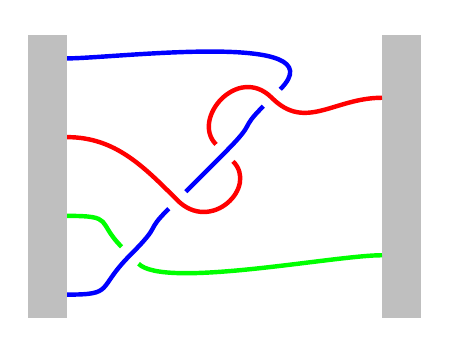
\begin{tikzpicture}
  \node (a) at ( 0.0, 1.5) {};
  \node (b) at ( 0.0, 0.5) {};
  \node (c) at ( 0.0,-0.5) {};
  \node (d) at ( 0.0,-1.5) {};
  \node (e) at ( 4.0, 1.0) {};
  \node (f) at ( 4.0,-1.0) {};
  \node (p) at ( 2.6, 1.0) {};
  \node (q) at ( 2.0, 0.3) {};
  \node (r) at ( 1.4,-0.3) {};
  \node (s) at ( 0.8,-1.0) {};
  
  \fill[lightgray] (-0.5,-1.8) rectangle ( 0.0, 1.8);
  \fill[lightgray] ( 4.0,-1.8) rectangle ( 4.5, 1.8);
  \draw[blue] 
   (a.center) .. controls (a.4 east) and (p.8 north east) ..
   (p)        .. controls (p.4 south west) and (q.4 north east) ..
   (q.center) .. controls (q.4 south west) and (r.4 north east) ..
   (r)        .. controls (r.4 south west) and (s.4 north east) ..
   (s.center) .. controls (s.4 south west) and (d.4 east) ..
   (d.center);
  \draw[red]
   (b.center) .. controls (b.4 east) and (r.4 north west) ..
   (r.center) .. controls (r.4 south east) and (q.4 south east) .. 
   (q)        .. controls (q.4 north west) and (p.4 north west) ..
   (p.center) .. controls (p.4 south east) and (e.4 west) ..
   (e.center);
  \draw[green]
   (c.center) .. controls (c.4 east) and (s.4 north west) ..
   (s)        .. controls (s.4 south east) and (f.4 west) ..
   (f.center);
 \end{tikzpicture}
\end{center}

\begin{center}
 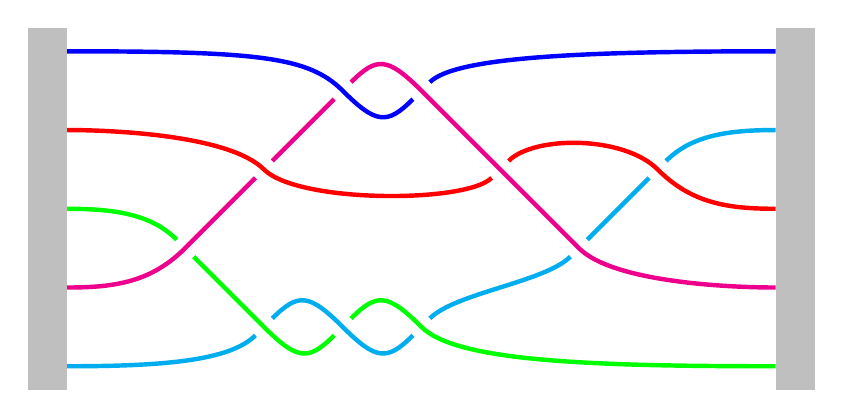
\begin{tikzpicture}
  \node (a) at (0, 2) {};
  \node (b) at (0, 1) {};
  \node (c) at (0, 0) {};
  \node (d) at (0,-1) {};
  \node (e) at (0,-2) {};
  \node (f) at (9, 2) {};
  \node (g) at (9, 1) {};
  \node (h) at (9, 0) {};
  \node (i) at (9,-1) {};
  \node (j) at (9,-2) {};
  \node (p) at ( 3.5, 1.5) {};
  \node (q) at ( 4.5, 1.5) {};
  \node (r) at ( 2.5, 0.5) {};
  \node (s) at ( 5.5, 0.5) {};
  \node (t) at ( 7.5, 0.5) {};
  \node (u) at ( 1.5,-0.5) {};
  \node (v) at ( 2.5,-1.5) {};
  \node (w) at ( 3.5,-1.5) {};
  \node (x) at ( 4.5,-1.5) {};
  \node (y) at ( 6.5,-0.5) {};

  \fill[lightgray] (-0.5,-2.3) rectangle ( 0.0, 2.3);
  \fill[lightgray] ( 9.0,-2.3) rectangle ( 9.5, 2.3);

  \draw[blue] 
   (a.center) .. controls (a.16 east) and (p.4 north west) ..
   (p.center) .. controls (p.4 south east) and (q.4 south west) ..
   (q)        .. controls (q.4 north east) and (f.16 west) ..
   (f.center);

  \draw[red]
   (b.center) .. controls (b.4 east) and (r.4 north west) ..
   (r.center) .. controls (r.4 south east) and (s.4 south west) ..
   (s)        .. controls (s.4 north east) and (t.4 north west) ..
   (t.center) .. controls (t.4 south east) and (h.4 west) ..
   (h.center);

  \draw[green] 
   (c.center) .. controls (c.4 east) and (u.4 north west) ..
   (u)        .. controls (u.4 south east) and (v.4 north west) ..
   (v.center) .. controls (v.4 south east) and (w.4 south west) ..
   (w)        .. controls (w.4 north east) and (x.4 north west) ..
   (x.center) .. controls (x.4 south east) and (j.16 west) ..
   (j.center);

  \draw[magenta] 
   (d.center) .. controls (d.4 east) and (u.4 south west) ..
   (u.center) .. controls (u.4 north east) and (r.4 south west) ..
   (r)        .. controls (r.4 north east) and (p.4 south west) ..
   (p)        .. controls (p.4 north east) and (q.4 north west) ..
   (q.center) .. controls (q.4 south east) and (s.4 north west) ..
   (s.center) .. controls (s.4 south east) and (y.4 north west) ..
   (y.center) .. controls (y.4 south east) and (i.4 west) ..
   (i.center);

  \draw[cyan] 
   (e.center) .. controls (e.8 east) and (v.4 south west) ..
   (v)        .. controls (v.4 north east) and (w.4 north west) ..
   (w.center) .. controls (w.4 south east) and (x.4 south west) ..
   (x)        .. controls (x.4 north east) and (y.4 south west) ..
   (y)        .. controls (y.4 north east) and (t.4 south west) ..
   (t)        .. controls (t.4 north east) and (g.4 west) ..
   (g.center);
 \end{tikzpicture}
\end{center}

\begin{center}
 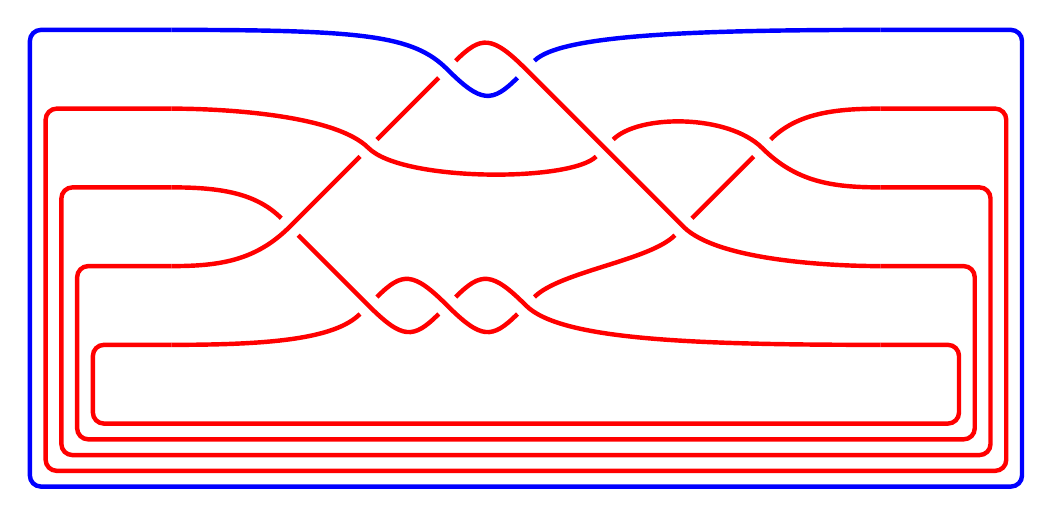
\begin{tikzpicture}
  \node (a) at (0, 2) {};
  \node (b) at (0, 1) {};
  \node (c) at (0, 0) {};
  \node (d) at (0,-1) {};
  \node (e) at (0,-2) {};
  \node (f) at (9, 2) {};
  \node (g) at (9, 1) {};
  \node (h) at (9, 0) {};
  \node (i) at (9,-1) {};
  \node (j) at (9,-2) {};
  \node (p) at ( 3.5, 1.5) {};
  \node (q) at ( 4.5, 1.5) {};
  \node (r) at ( 2.5, 0.5) {};
  \node (s) at ( 5.5, 0.5) {};
  \node (t) at ( 7.5, 0.5) {};
  \node (u) at ( 1.5,-0.5) {};
  \node (v) at ( 2.5,-1.5) {};
  \node (w) at ( 3.5,-1.5) {};
  \node (x) at ( 4.5,-1.5) {};
  \node (y) at ( 6.5,-0.5) {};

  \draw
   (a.center) .. controls (a.16 east) and (p.4 north west) ..
   (p.center) .. controls (p.4 south east) and (q.4 south west) ..
   (q)        .. controls (q.4 north east) and (f.16 west) ..
   (f.center);

  \draw[red]
   (b.center) .. controls (b.4 east) and (r.4 north west) ..
   (r.center) .. controls (r.4 south east) and (s.4 south west) ..
   (s)        .. controls (s.4 north east) and (t.4 north west) ..
   (t.center) .. controls (t.4 south east) and (h.4 west) ..
   (h.center);

  \draw[red]
   (c.center) .. controls (c.4 east) and (u.4 north west) ..
   (u)        .. controls (u.4 south east) and (v.4 north west) ..
   (v.center) .. controls (v.4 south east) and (w.4 south west) ..
   (w)        .. controls (w.4 north east) and (x.4 north west) ..
   (x.center) .. controls (x.4 south east) and (j.16 west) ..
   (j.center);

  \draw[red]
   (d.center) .. controls (d.4 east) and (u.4 south west) ..
   (u.center) .. controls (u.4 north east) and (r.4 south west) ..
   (r)        .. controls (r.4 north east) and (p.4 south west) ..
   (p)        .. controls (p.4 north east) and (q.4 north west) ..
   (q.center) .. controls (q.4 south east) and (s.4 north west) ..
   (s.center) .. controls (s.4 south east) and (y.4 north west) ..
   (y.center) .. controls (y.4 south east) and (i.4 west) ..
   (i.center);

  \draw[red]
   (e.center) .. controls (e.8 east) and (v.4 south west) ..
   (v)        .. controls (v.4 north east) and (w.4 north west) ..
   (w.center) .. controls (w.4 south east) and (x.4 south west) ..
   (x)        .. controls (x.4 north east) and (y.4 south west) ..
   (y)        .. controls (y.4 north east) and (t.4 south west) ..
   (t)        .. controls (t.4 north east) and (g.4 west) ..
   (g.center);

  \draw[rounded corners] (0, 2) -- (-1.8, 2) -- (-1.8,-3.8) -- (10.8,-3.8) -- (10.8, 2) -- (9, 2);
  \draw[red,rounded corners] (0, 1) -- (-1.6, 1) -- (-1.6,-3.6) -- (10.6,-3.6) -- (10.6, 1) -- (9, 1);
  \draw[red,rounded corners] (0, 0) -- (-1.4, 0) -- (-1.4,-3.4) -- (10.4,-3.4) -- (10.4, 0) -- (9, 0);
  \draw[red,rounded corners] (0,-1) -- (-1.2,-1) -- (-1.2,-3.2) -- (10.2,-3.2) -- (10.2,-1) -- (9,-1);
  \draw[red,rounded corners] (0,-2) -- (-1,-2) -- (-1,-3) -- (10,-3) -- (10,-2) -- (9,-2);
 \end{tikzpicture}
\end{center}

\begin{center}
 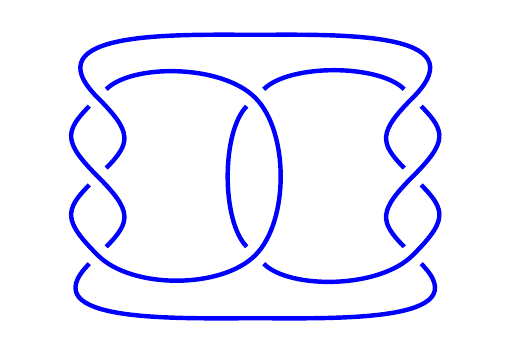
\begin{tikzpicture}
  \node (a) at (-2, 1) {};
  \node (b) at (-2, 0) {};
  \node (c) at (-2,-1) {};
  \node (d) at ( 0, 1) {};
  \node (e) at ( 0,-1) {};
  \node (f) at ( 2, 1) {};
  \node (g) at ( 2, 0) {};
  \node (h) at ( 2,-1) {};
  \draw
   (a.center) .. controls (a.4 south east) and (b.4 north east) ..
   (b)        .. controls (b.4 south west) and (c.4 north west) ..
   (c.center) .. controls (c.4 south east) and (e.4 south west) ..
   (e.center) .. controls (e.4 north east) and (d.4 south east) ..
   (d.center) .. controls (d.4 north west) and (a.4 north east) ..
   (a)        .. controls (a.4 south west) and (b.4 north west) ..
   (b.center) .. controls (b.4 south east) and (c.4 north east) ..
   (c)        .. controls (c.8 south west) and (-1,-1.8) ..
   (0,-1.8)   .. controls (1,-1.8) and (h.8 south east) ..
   (h)        .. controls (h.4 north west) and (g.4 south west) ..
   (g.center) .. controls (g.4 north east) and (f.4 south east) ..
   (f)        .. controls (f.4 north west) and (d.4 north east) ..
   (d)        .. controls (d.4 south west) and (e.4 north west) ..
   (e)        .. controls (e.4 south east) and (h.4 south west) ..
   (h.center) .. controls (h.4 north east) and (g.4 south east) ..
   (g)        .. controls (g.4 north west) and (f.4 south west) ..
   (f.center) .. controls (f.8 north east) and (1,1.8) ..
   (0, 1.8)   .. controls (-1,1.8) and (a.8 north west) .. (a.center);
 \end{tikzpicture}
\end{center}

\begin{center}
 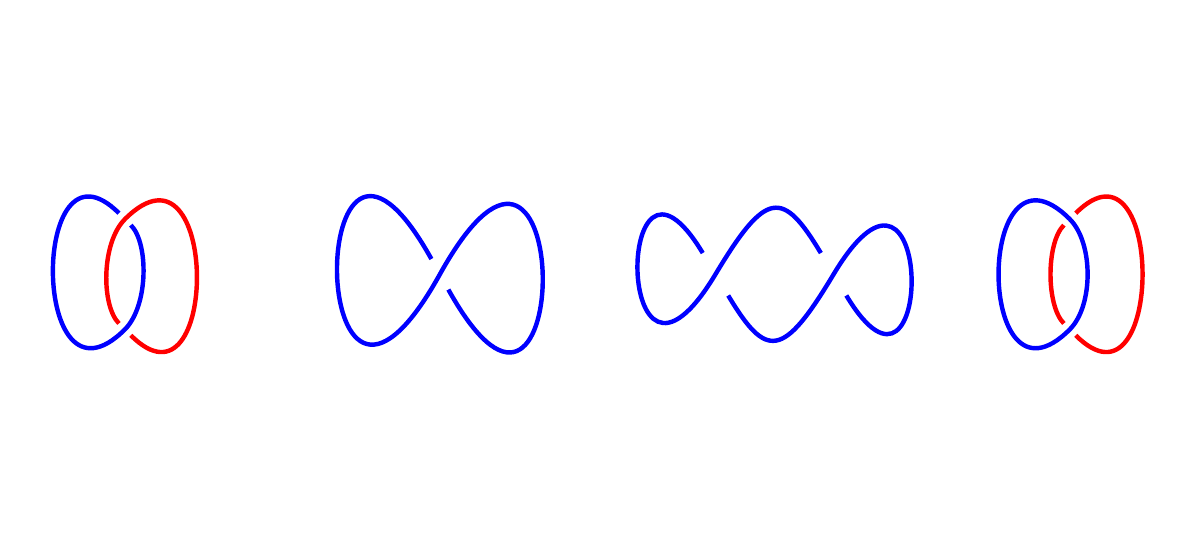
\begin{tikzpicture}
  \begin{scope}[scale=0.7]
   \node (a) at ( 0.00, 1.00) {};
   \node (b) at ( 0.00,-1.00) {};
   \draw[blue] (a) .. controls (a.4 south east) and (b.4 north east) ..
               (b.center) .. controls (b.16 south west) and (a.16 north west) .. (a);
   \draw[red]  (a.center) .. controls (a.4 south west) and (b.4 north west) ..
               (b) .. controls (b.16 south east) and (a.16 north east) .. (a.center);
  \end{scope}
  \begin{scope}[xshift=4cm,yscale=1.8]
   \node (a) at (0,0) {};
   \draw (a.center) .. controls (a.16 north east) and (a.16 south east) ..
         (a) .. controls (a.16 north west) and (a.16 south west) .. (a.center);
  \end{scope}
  \begin{scope}[xshift=7.5cm,xscale=1.5,yscale=2.5]
   \node (a) at (0,0) {};
   \node (b) at (1,0) {};
   \draw (a.center) .. controls (a.4 north east) and (b.4 north west) ..
         (b)        .. controls (b.8 south east) and (b.8 north east) ..
         (b.center) .. controls (b.4 south west) and (a.4 south east) .. 
         (a)        .. controls (a.8 north west) and (a.8 south west) .. (a.center);
  \end{scope}
  \begin{scope}[xshift=12cm,scale=0.7]
   \node (a) at ( 0.00, 1.00) {};
   \node (b) at ( 0.00,-1.00) {};
   \draw[blue] (a.center) .. controls (a.4 south east) and (b.4 north east) ..
               (b.center) .. controls (b.16 south west) and (a.16 north west) .. (a.center);
   \draw[red]  (a) .. controls (a.4 south west) and (b.4 north west) ..
               (b) .. controls (b.16 south east) and (a.16 north east) .. (a);
  \end{scope}
 \end{tikzpicture}
\end{center}

\begin{center}
 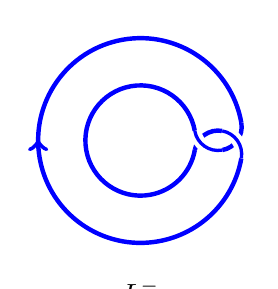
\begin{tikzpicture}
  \draw (0,0) (10:1.3) arc(10:350:1.3);
  \draw (0,0) (10:0.7) arc(10:350:0.7);
  \draw (350:1) +( 80:0.3) arc( 80:170:0.3);
  \draw ( 10:1) +(280:0.3) arc(280:370:0.3);
  \draw[draw=white,double=blue,double distance=1.2pt] (350:1) +(350:0.3) arc(-10: 80:0.3);
  \draw[draw=white,double=blue,double distance=1.2pt] ( 10:1) +(190:0.3) arc(190:280:0.3);
  \draw[->] (180:1.3) -- +(90:0.01);
  \draw[black] (0,-1.5) node[anchor=north] {$L_1^-$};
 \end{tikzpicture}
 \hspace{5em}
 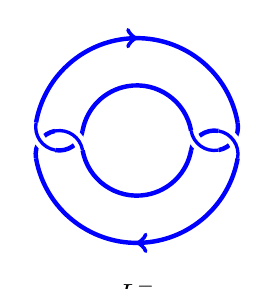
\begin{tikzpicture}
  \foreach \t in {0,180} {
   \begin{scope}[rotate=\t]
    \draw (0,0) ( 10:1.3) arc( 10:170:1.3);
    \draw (0,0) ( 10:0.7) arc( 10:170:0.7);
    \draw (350:1) +( 80:0.3) arc( 80:170:0.3);
    \draw ( 10:1) +(280:0.3) arc(280:370:0.3);
    \draw[draw=white,double=blue,double distance=1.2pt] (350:1) +(350:0.3) arc(-10: 80:0.3);
    \draw[draw=white,double=blue,double distance=1.2pt] ( 10:1) +(190:0.3) arc(190:280:0.3);
    \draw[->] (90:1.3) -- +( 0:0.01);
   \end{scope}
  }
  \draw[black] (0,-1.5) node[anchor=north] {$L_2^-$};
 \end{tikzpicture}
 \hspace{5em}
 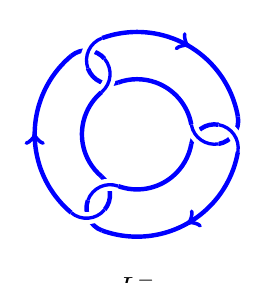
\begin{tikzpicture}
  \foreach \t in {0,120,240} {
   \begin{scope}[rotate=\t]
    \draw (0,0) ( 10:1.3) arc( 10:110:1.3);
    \draw (0,0) ( 10:0.7) arc( 10:110:0.7);
    \draw (350:1) +( 80:0.3) arc( 80:170:0.3);
    \draw ( 10:1) +(280:0.3) arc(280:370:0.3);
    \draw[draw=white,double=blue,double distance=1.2pt] (350:1) +(350:0.3) arc(-10: 80:0.3);
    \draw[draw=white,double=blue,double distance=1.2pt] ( 10:1) +(190:0.3) arc(190:280:0.3);
    \draw[->] (60:1.3) -- +(-30:0.01);
   \end{scope}
  }
  \draw[black] (0,-1.5) node[anchor=north] {$L_3^-$};
 \end{tikzpicture}
\end{center}

\begin{center}
 \begin{tikzpicture}
  \def\r{0.8}
  \foreach \x in {0.0,1.0,2.0,3.0,4.0,5.0} {
   \draw[draw=white,double=blue,double distance=1.2pt] (\x,0) +( \r,0) arc(0:180:\r);
   \draw[->] (\x,\r) -- +(0.01,0);
  }
  \foreach \x in {5.0,4.0,3.0,2.0,1.0,0.0}
   \draw[draw=white,double=blue,double distance=1.2pt] (\x,0) +(-\r,0) arc(180:360:\r);
  \draw[black] (-1,0) node[anchor=east] {$C_6=$};
 \end{tikzpicture}
\end{center}

\begin{center}
 \begin{tikzpicture}
  \fill[lightgray] (-1.2,-1.2) rectangle (1.2,1.2);
  \draw (1.2,-1) -- (1.5,-1);
  \draw (1.2, 1) -- (1.5, 1);
  \draw (1.5,0) (1.5, 1) arc ( 90:0:1);
  \draw[draw=white,double=red ,double distance=1.2pt] (2.5,0) circle(1);
  \draw[draw=white,double=blue,double distance=1.2pt] (1.5,0) (1.5,-1) arc (-90:0:1);
  \draw[red ,->] (3.5,0) -- (3.5,-0.01);
  \draw[blue,->] (2.5,0) -- (2.5,-0.01);
  \draw[black] (0,0) node{$L$};
 \end{tikzpicture}
\end{center}

\begin{center}
 \begin{tikzpicture}[scale=2,every path/.style={blue,very thick},
    every node/.style={transform shape, knot crossing, inner sep=2.5pt}]
  \node (a) at ( 0.00, 0.75) {};
  \node (b) at ( 0.00, 0.25) {};
  \node (c) at ( 0.00,-0.25) {};
  \node (d) at ( 0.00,-0.75) {};
  \draw[blue] (-0.5,1.0) .. controls (-0.4,1.0) and (a.2 north west) .. (a.center) 
   .. controls (a.2 south east) and (b.2 north east) .. (b) 
   .. controls (b.2 south west) and (c.2 north west) .. (c.center) 
   .. controls (c.2 south east) and (d.2 north east) .. (d)
   .. controls (d.2 south west) and (-0.4,-1.0) .. (-0.5,-1.0);
  \draw[blue,rounded corners] (-0.5,-1.0) -- (-0.75,-1.0) -- (-0.75,1.0) -- (-0.5,1.0);
  \draw[red ] ( 0.5,1.0) .. controls ( 0.4,1.0) and (a.2 north east) .. (a) 
   .. controls (a.2 south west) and (b.2 north west) .. (b.center) 
   .. controls (b.2 south east) and (c.2 north east) .. (c) 
   .. controls (c.2 south west) and (d.2 north west) .. (d.center)
   .. controls (d.2 south east) and ( 0.4,-1.0) .. ( 0.5,-1.0);
  \draw[red ,rounded corners] ( 0.5,-1.0) -- ( 0.75,-1.0) -- ( 0.75,1.0) -- ( 0.5,1.0);
  \draw[blue,->] (-0.75,0) -- (-0.75,-0.01);
  \draw[red ,->] ( 0.75,0) -- ( 0.75,-0.01);
 \end{tikzpicture}
\end{center}

\begin{center}
 \begin{tikzpicture}
  \node (a) at (0,1) {};
  \node (b) at (2,1) {};
  \node (c) at (3,1) {};
  \node (d) at (1,0) {};
  \node (e) at (2,0) {};
  \node (f) at (3,0) {};
  \draw 
   (b)        .. controls (b.4 north east) and (c.4 north west) ..
   (c.center) .. controls (c.4 south) and (f.4 north) ..
   (f.center) .. controls (f.4 south west) and (e.4 south east) ..
   (e)        .. controls (e.4 north) and (b.4 south) ..
   (b);
  \draw 
   (a)        .. controls (a.8 north east) and (b.8 west) ..
   (b.center) .. controls (b.8 east) and (c.8 west) ..
   (c)        .. controls (c.8 east) .. (3.2,1);
  \draw[rounded corners]
   (3.2,1) -- (4,1) -- (4,3) -- (-1,3) -- (-1,1) -- (-0.8,1);
  \draw
   (-0.8,1) .. controls (-0.1,1) and (a.8 west) ..
   (a.center) .. controls (a.8 east) and (d.8 north) ..
   (d)        .. controls (d.2 south) .. (1,-0.2);
  \draw[rounded corners]
   (1,-0.2) -- (1,-0.5) -- (-1.5,-0.5) -- (-1.5,3.5) -- (4.5,3.5) -- (4.5,0) -- (3.5,0);
  \draw 
   (3.5,0) .. controls (f.4 east) .. 
   (f) .. controls (e.4 east) ..
   (e.center) .. controls (d.4 east) ..
   (d.center) .. controls (d.4 west) and (a.4 south) .. (a);
  \draw[->] (1.5,3.5) -- (1.51,3.5);
  \draw[->] (3.0,0.5) -- (3.0,0.49);
 \end{tikzpicture}
\end{center}

\begin{center}
 \begin{tikzpicture}[scale=0.5]
  \begin{scope}
   \node (p) at (-5, 0) {};
   \node (q) at ( 5, 0) {};
   \node (a) at (-2, 1) {};
   \node (b) at ( 0, 1) {};
   \node (c) at ( 2, 1) {};
   \node (d) at (-2,-1) {};
   \node (e) at ( 0,-1) {};
   \node (f) at ( 2,-1) {};
   \draw 
    (a)        .. controls (a.8 south east) and (b.8 south west) ..
    (b.center) .. controls (b.8 north east) and (c.8 north west) ..
    (c)        .. controls (c.8 south east) and (f.8 north east) ..
    (f)        .. controls (f.8 south west) and (e.8 south east) ..
    (e.center) .. controls (e.8 north west) and (d.8 north east) ..
    (d)        .. controls (d.8 south west) and (p.16 south) ..
    (p.center) .. controls (p.16 north) and (a.8 north west) ..
    (a);
   \draw 
    (c.center) .. controls (c.8 south west) and (b.8 south east) ..
    (b)        .. controls (b.8 north west) and (a.8 north east) ..
    (a.center) .. controls (a.8 south west) and (d.8 north west) ..
    (d.center) .. controls (d.8 south east) and (e.8 south west) ..
    (e)        .. controls (e.8 north east) and (f.8 north west) ..
    (f.center) .. controls (f.8 south east) and (q.16 south) ..
    (q.center) .. controls (q.16 north) and (c.8 north east) ..
    (c.center);
   \draw (-3.6,0) circle(0.7);
   \draw ( 3.6,0) circle(0.7);
  \end{scope}
  \draw (7,0) node{\Huge and };
  \begin{scope}[xshift=10cm,draw=red]
   \draw[red] (0.0,0) circle(1);
   \draw[red] (2.4,0) circle(1);
   \draw[red] (4.8,0) circle(1);
   \draw[red] (7.2,0) circle(1);
  \end{scope}
 \end{tikzpicture}
\end{center}

\begin{center}
 \begin{tikzpicture}[scale=0.5]
  \begin{scope}
   \draw[red] (0,0) circle(2);  
   \node (a) at (0,0) {};
   \draw (a) .. controls (a.16 north east) and (a.16 north west) ..
         (a.center) .. controls (a.16 south east) and (a.16 south west) .. (a);
  \end{scope}
  \draw[dotted,black] (4,-2) -- (4,2);
  \begin{scope}[xshift=8cm,scale=2]
   \node (a) at ( 1,0) {};
   \node (b) at (-1,0) {};
   \draw[red] (a) .. controls (a.8 north east) and (b.8 north) ..
         (b.center) .. controls (b.8 south) and (a.8 south east) .. 
         (a.center) .. controls (a.8 north west) and (a.8 south west) .. (a);
   \begin{scope}[xshift=-0.4cm,scale=0.3]
    \node (a) at ( 1,0) {};
    \node (b) at (-1,0) {};
    \draw (a) .. controls (a.8 north east) and (b.8 north) ..
          (b.center) .. controls (b.8 south) and (a.8 south east) .. 
          (a.center) .. controls (a.8 north west) and (a.8 south west) .. (a);
   \end{scope}
  \end{scope}
  \begin{scope}[xshift=14cm]
   \begin{scope}
    \node (a) at (0,0) {};
    \draw[red] (a) .. controls (a.16 north east) and (a.16 north west) ..
          (a.center) .. controls (a.16 south east) and (a.16 south west) .. (a);
   \end{scope}
   \begin{scope}[xshift=2cm]
    \node (a) at (0,0) {};
    \draw (a.center) .. controls (a.16 north east) and (a.16 north west) ..
          (a) .. controls (a.16 south east) and (a.16 south west) .. (a.center);
   \end{scope}   
  \end{scope}
  \draw[dotted,black] (12,-2) -- (12,2);
 \end{tikzpicture}
\end{center}

\begin{center}
 \begin{tikzpicture}
  \begin{scope}
   \draw (0,0) circle(1);
  \end{scope}
  \begin{scope}[xshift=3cm]
   \node (a) at (0,0) {};
   \draw (a) .. controls (a.16 north east) and (a.16 north west) ..
         (a.center) .. controls (a.16 south east) and (a.16 south west) .. (a);
  \end{scope}
  \begin{scope}[xshift=6cm]
   \node (a) at (0,0) {};
   \draw (a.center) .. controls (a.16 north east) and (a.16 north west) ..
         (a) .. controls (a.16 south east) and (a.16 south west) .. (a.center);
  \end{scope}
  \begin{scope}[xshift=12cm]
   \node (a) at ( 1,0) {};
   \node (b) at (-1,0) {};
   \draw (a) .. controls (a.8 north east) and (b.8 north) ..
         (b.center) .. controls (b.8 south) and (a.8 south east) .. 
         (a.center) .. controls (a.8 north west) and (a.8 south west) .. (a);
  \end{scope}
  \begin{scope}[xshift=9cm]
   \node (a) at ( 1,0) {};
   \node (b) at (-1,0) {};
   \draw (a.center) .. controls (a.8 north east) and (b.8 north) ..
         (b.center) .. controls (b.8 south) and (a.8 south east) .. 
         (a) .. controls (a.8 north west) and (a.8 south west) .. (a.center);
  \end{scope}
 \end{tikzpicture}
\end{center}

\begin{center}
 \begin{tikzpicture}[scale=0.7]
  \node (a) at (-6,0) {};
  \node (b) at (-4,0) {};
  \node (c) at (-2,0) {};
  \node (d) at ( 2,0) {};
  \node (e) at ( 4,0) {};
  \node (f) at ( 6,0) {};
  \draw 
   (1.5,-0.5) .. controls (d.4 south west) .. 
   (d)        .. controls (d.4 north east) and (e.4 north west) ..
   (e.center) .. controls (e.4 south east) and (f.4 south west) ..
   (f)        .. controls (f.4 north east) .. (6.5,0.5);
  \draw[rounded corners] (6.5,0.5) -- (6.5,4) -- (-6.5,4) -- (-6.5,0.5);
  \draw
   (-6.5,0.5) .. controls (a.4 north west) ..
   (a.center) .. controls (a.4 south east) and (b.4 south west) ..
   (b) .. controls (b.4 north east) and (c.4 north west) ..
   (c.center) .. controls (c.4 south east) .. (-1.5,-0.5);
  \draw 
   (1.5, 0.5) .. controls (d.4 north west) .. 
   (d.center) .. controls (d.4 south east) and (e.4 south west) ..
   (e)        .. controls (e.4 north east) and (f.4 north west) ..
   (f.center) .. controls (f.4 south east) .. (6.5,-0.5);
  \draw[rounded corners] (6.5,-0.5) -- (7,-0.5) -- (7,4.5) -- (-7,4.5) -- (-7,-0.5) -- (-6.5,-0.5);
  \draw
   (-6.5,-0.5) .. controls (a.4 south west) ..
   (a) .. controls (a.4 north east) and (b.4 north west) ..
   (b.center) .. controls (b.4 south east) and (c.4 south west) ..
   (c) .. controls (c.4 north east) .. (-1.5, 0.5);
  \fill[black] (-1.2,0) circle(0.1);
  \fill[black] (-0.8,0) circle(0.1);
  \fill[black] (-0.4,0) circle(0.1);
  \fill[black] ( 0.0,0) circle(0.1);
  \fill[black] ( 0.4,0) circle(0.1);
  \fill[black] ( 0.8,0) circle(0.1);
  \fill[black] ( 1.2,0) circle(0.1);
 \end{tikzpicture}
\end{center}

\begin{center}
 \begin{tikzpicture}[scale=0.7]
  \node (a) at (-6,0) {};
  \node (b) at (-4,0) {};
  \node (c) at (-2,0) {};
  \node (d) at ( 2,0) {};
  \node (e) at ( 4,0) {};
  \node (f) at ( 6,0) {};
  \node (g) at ( 0.3,5.0) {};
  \node (h) at (-0.3,3.5) {};
  \draw 
   (1.5,-0.5) .. controls (d.4 south west) .. 
   (d)        .. controls (d.4 north east) and (e.4 north west) ..
   (e.center) .. controls (e.4 south east) and (f.4 south west) ..
   (f)        .. controls (f.4 north east) .. (6.5,0.5);
  \draw[rounded corners] (6.5,0.5) -- (6.5,4) -- (2,4); 
  \draw[rounded corners] (-2,4) -- (-6.5,4) -- (-6.5,0.5);
  \draw
   (-6.5,0.5) .. controls (a.4 north west) ..
   (a.center) .. controls (a.4 south east) and (b.4 south west) ..
   (b) .. controls (b.4 north east) and (c.4 north west) ..
   (c.center) .. controls (c.4 south east) .. (-1.5,-0.5);
  \draw 
   (1.5, 0.5) .. controls (d.4 north west) .. 
   (d.center) .. controls (d.4 south east) and (e.4 south west) ..
   (e)        .. controls (e.4 north east) and (f.4 north west) ..
   (f.center) .. controls (f.4 south east) .. (6.5,-0.5);
  \draw[rounded corners] (6.5,-0.5) -- (7,-0.5) -- (7,4.5) -- (2,4.5);
  \draw[rounded corners] (-2,4.5) -- (-7,4.5) -- (-7,-0.5) -- (-6.5,-0.5);
  \draw
   (-6.5,-0.5) .. controls (a.4 south west) ..
   (a) .. controls (a.4 north east) and (b.4 north west) ..
   (b.center) .. controls (b.4 south east) and (c.4 south west) ..
   (c) .. controls (c.4 north east) .. (-1.5, 0.5);
  \draw
   (2,4.5) .. controls (1,4.5) and (g.4 north east) ..
   (g) .. controls (g.4 south west) and (h.4 north west) ..
   (h.center) .. controls (h.4 east) and (1,4) .. (2,4); 
  \draw
   (-2,4.5) .. controls (-1,4.5) and (g.4 west) ..
   (g.center) .. controls (g.4 south east) and (h.4 north east) ..
   (h) .. controls (h.4 south west) and (-1,4) .. (-2,4); 
  \fill[black] (-1.2,0) circle(0.1);
  \fill[black] (-0.8,0) circle(0.1);
  \fill[black] (-0.4,0) circle(0.1);
  \fill[black] ( 0.0,0) circle(0.1);
  \fill[black] ( 0.4,0) circle(0.1);
  \fill[black] ( 0.8,0) circle(0.1);
  \fill[black] ( 1.2,0) circle(0.1);
 \end{tikzpicture}
\end{center}

% Hopf link
\begin{center}
 \begin{tikzpicture}
  \node (a) at ( 0.00, 1.00) {};
  \node (b) at ( 0.00,-1.00) {};
  \draw[blue] (a.center) .. controls (a.4 south east) and (b.4 north east) ..
              (b) .. controls (b.16 south west) and (a.16 north west) .. (a.center);
  \draw[red]  (a) .. controls (a.4 south west) and (b.4 north west) ..
              (b.center) .. controls (b.16 south east) and (a.16 north east) .. (a);
  \draw[red ,->] (-0.31,0) -- (-0.31, 0.01);
  \draw[blue,->] ( 0.31,0) -- ( 0.31,-0.01);
 \end{tikzpicture}
\end{center}

% Unlink
\begin{center}
 \begin{tikzpicture}
  \node (a) at ( 0.00, 1.00) {};
  \node (b) at ( 0.00,-1.00) {};
  \draw[blue] (a.center) .. controls (a.4 south east) and (b.4 north east) ..
              (b.center) .. controls (b.16 south west) and (a.16 north west) .. (a.center);
  \draw[red]  (a) .. controls (a.4 south west) and (b.4 north west) ..
              (b) .. controls (b.16 south east) and (a.16 north east) .. (a);
 \end{tikzpicture}
\end{center}

% Long overhand knot
\begin{center}
 \begin{tikzpicture}
  \node (a) at (-1.00, 0.00) {};
  \node (b) at ( 1.00, 0.00) {};
  \node (c) at ( 0.00, 0.50) {};
  \draw (-4,0) -- (a)
    .. controls (a.2 east) and (c.south west) .. (c.center)
    .. controls (c.4 north east) and (b.4 north) .. (b)
    .. controls (b.8 south) and (a.8 south) .. (a.center)
    .. controls (a.4 north) and (c.4 north west) .. (c)
    .. controls (c.south east) and (b.2 west) .. (b.center)
    -- (4,0);
 \end{tikzpicture}
\end{center}

% Closed overhand knot
\begin{center}
 \begin{tikzpicture}[every path/.style={blue,very thick}, every node/.style={transform shape, knot crossing, inner sep=2.5pt}]
  \node (a) at (-1.00, 0.00) {};
  \node (b) at ( 1.00, 0.00) {};
  \node (c) at ( 0.00, 0.50) {};
  \draw (-4,0) -- (a)
    .. controls (a.2 east) and (c.south west) .. (c.center)
    .. controls (c.4 north east) and (b.4 north) .. (b)
    .. controls (b.8 south) and (a.8 south) .. (a.center)
    .. controls (a.4 north) and (c.4 north west) .. (c)
    .. controls (c.south east) and (b.2 west) .. (b.center)
    -- (4,0);
  \draw[rounded corners]
   (4,0) -- (4.2,0) -- (4.2,1.5) -- (-4.2,1.5) -- (-4.2,0) -- (-4,0);
 \end{tikzpicture}
\end{center}

% Unknot
\begin{center}
 \begin{tikzpicture}
  \draw (0,0) circle (1.2);
 \end{tikzpicture}
\end{center}

\begin{center}
 \begin{tikzpicture}
  \node (a) at ( 0.00, 1.00) {};
  \node (b) at ( 0.00, 0.00) {};
  \node (c) at ( 0.00,-1.00) {};
  \draw (a.center) 
   .. controls (a.4 south east) and (b.4 north east) .. (b) 
   .. controls (b.4 south west) and (c.4 north west) .. (c.center) 
   .. controls (c.8 south east) and (a.8 north east) .. (a)
   .. controls (a.4 south west) and (b.4 north west) .. (b.center)
   .. controls (b.4 south east) and (c.4 north east) .. (c)
   .. controls (c.8 south west) and (a.8 north west) .. (a.center);
 \end{tikzpicture}
\end{center}

% Trefoil
\begin{center}
 \begin{tikzpicture}
  \begin{scope}[rotate=  0] \node (a) at (0,-1) {}; \end{scope}
  \begin{scope}[rotate=120] \node (b) at (0,-1) {}; \end{scope}
  \begin{scope}[rotate=240] \node (c) at (0,-1) {}; \end{scope}
  \draw (a) .. controls (a.4 north west) and (c.4 north east) .. (c.center);
  \draw (b) .. controls (b.4 north west) and (a.4 north east) .. (a.center);
  \draw (c) .. controls (c.4 north west) and (b.4 north east) .. (b.center);
  \draw (a.center) .. controls (a.16 south west) and (c.16 south east) .. (c);
  \draw (b.center) .. controls (b.16 south west) and (a.16 south east) .. (a);
  \draw (c.center) .. controls (c.16 south west) and (b.16 south east) .. (b);
  \draw[->] (0,2.2) -- (0.01,2.2);
 \end{tikzpicture}
\end{center}

% Eight
\begin{center}
 \begin{tikzpicture}
  \node (a) at (-0.50, 1.00) {};
  \node (b) at ( 0.50, 1.00) {};
  \node (c) at ( 0.00, 0.00) {};
  \node (d) at ( 0.00,-1.00) {};
  \draw (a) -- (b.center) 
   .. controls (b.8 east) and (d.8 south east) .. (d)
   .. controls (d.4 north west) and (c.4 south west) .. (c.center)
   .. controls (c.4 north east) and (b.4 south) .. (b)
   .. controls (b.4 north) and (a.4 north) .. (a.center)
   .. controls (a.4 south) and (c.4 north west) .. (c)
   .. controls (c.4 south east) and (d.4 north east) ..(d.center)
   .. controls (d.8 south west) and (a.8 west) .. (a); 
 \end{tikzpicture}
\end{center}

\begin{center}
 \begin{tikzpicture}[scale=1.2,every path/.style={blue,very thick},
    every node/.style={transform shape, knot crossing, inner sep=2.5pt}]
  \node (a) at (-1.00, 1.00) {};
  \node (b) at ( 1.00, 1.00) {};
  \node (c) at ( 0.00, 0.00) {};
  \node (d) at (-1.00,-1.00) {};
  \node (e) at ( 1.00,-1.00) {};
  \node (f) at ( 0.00,-2.00) {};
  \draw (a) -- (c.center) -- (e)
   .. controls (e.4 south east) and (f.4 south east) .. (f) -- (d.center)
   .. controls (d.4 north west) and (a.4 south west) .. (a.center) 
   .. controls (a.4 north east) and (b.4 north west) .. (b.center) 
   .. controls (b.4 south east) and (e.4 north east) .. (e.center) -- (f.center)
   .. controls (f.4 south west) and (d.4 south west) .. (d) 
   -- (c) -- (b) 
   .. controls (b.8 north east) and (a.8 north west) .. (a);
 \end{tikzpicture}
\end{center}

% Pentagram
\begin{center}
 \begin{tikzpicture}[scale=1,every path/.style={blue,very thick},
     every node/.style={transform shape, knot crossing, inner sep=2.5pt}]

  \begin{scope}[rotate=  0] \node (a) at (0,-1.5) {}; \end{scope}
  \begin{scope}[rotate= 72] \node (b) at (0,-1.5) {}; \end{scope}
  \begin{scope}[rotate=144] \node (c) at (0,-1.5) {}; \end{scope}
  \begin{scope}[rotate=216] \node (d) at (0,-1.5) {}; \end{scope}
  \begin{scope}[rotate=288] \node (e) at (0,-1.5) {}; \end{scope}

  \draw (0,0) 
   (a) .. controls (a.16 south east) and (b.16 south west) .. (b.center) .. controls (b.4 north east) and (c.4 north west) ..
   (c) .. controls (c.16 south east) and (d.16 south west) .. (d.center) .. controls (d.4 north east) and (e.4 north west) ..
   (e) .. controls (e.16 south east) and (a.16 south west) .. (a.center) .. controls (a.4 north east) and (b.4 north west) ..
   (b) .. controls (b.16 south east) and (c.16 south west) .. (c.center) .. controls (c.4 north east) and (d.4 north west) ..
   (d) .. controls (d.16 south east) and (e.16 south west) .. (e.center) .. controls (e.4 north east) and (a.4 north west) ..
   (a); 
 \end{tikzpicture}
\end{center}

% Reidemeister 1
\begin{center}
 \begin{tikzpicture}[scale=0.8]
  \node (a) {};
  \draw (a.center) .. controls (a.32 north east) and (a.32 south east) .. (a);
  \draw (a.center) -- (a.8 south west);
  \draw (a) -- (a.8 north west);
  \draw[double=none,black,<->] (3,0) -- ++(1.5,0);
  \begin{scope}[xshift=6cm]
   \node (b) {};
   \draw (b.8 north west) -- (b.4 north west) to[out=-45,in=-135] (b.4 north east) .. controls (b.32 north east) and (b.32 south east) .. (b.4 south east) to[out=135,in=45] (b.4 south west) -- (b.8 south west);
   \draw[double=none,black,<->] (3,0) -- ++(1.5,0);
  \end{scope}
  \begin{scope}[xshift=12cm]
   \node[rotate=90] (c) {};
   \draw (c.center) .. controls (c.32 south west) and (c.32 south east) .. (c);
   \draw (c.center) -- (c.8 north east);
   \draw (c) -- (c.8 north west);
  \end{scope}
 \end{tikzpicture}
\end{center}

% Reidemeister 2
\begin{center}
 \begin{tikzpicture}
  \begin{scope}
   \node (a) at (-1, 2) {};
   \node (b) at ( 1, 2) {};
   \node (c) at ( 0, 1) {};
   \node (d) at ( 0,-1) {};
   \node (e) at (-1,-2) {};
   \node (f) at ( 1,-2) {};
   \draw (a) .. controls (a.4 south east) and (c.4 north west) .. 
         (c) .. controls (c.4 south east) and (d.4 north east) ..
         (d) .. controls (d.4 south west) and (e.4 north east) .. (e);
   \draw (b) ..        controls (b.4 south west) and (c.4 north east) .. 
         (c.center) .. controls (c.4 south west) and (d.4 north west) ..
         (d.center) .. controls (d.4 south east) and (f.4 north west) .. (f);
  \end{scope}
  \begin{scope}[xshift=5cm]
   \node (a) at (-1, 2) {};
   \node (b) at ( 1, 2) {};
   \node (c) at ( 0, 1) {};
   \node (d) at ( 0,-1) {};
   \node (e) at (-1,-2) {};
   \node (f) at ( 1,-2) {};
   \draw (a) .. controls (-0.3, 0.5) and (-0.3,-0.5) .. (e);
   \draw (b) .. controls ( 0.3, 0.5) and ( 0.3,-0.5) .. (f);
  \end{scope}
  \begin{scope}[xshift=10cm]
   \node (a) at (-1, 2) {};
   \node (b) at ( 1, 2) {};
   \node (c) at ( 0, 1) {};
   \node (d) at ( 0,-1) {};
   \node (e) at (-1,-2) {};
   \node (f) at ( 1,-2) {};
   \draw (a)        .. controls (a.4 south east) and (c.4 north west) .. 
         (c.center) .. controls (c.4 south east) and (d.4 north east) ..
         (d.center) .. controls (d.4 south west) and (e.4 north east) .. (e);
   \draw (b) ..        controls (b.4 south west) and (c.4 north east) .. 
         (c) .. controls (c.4 south west) and (d.4 north west) ..
         (d) .. controls (d.4 south east) and (f.4 north west) .. (f);
  \end{scope}
 \end{tikzpicture}
\end{center}

% Reidemeister 3
\begin{center}
 \begin{tikzpicture}[scale=0.9]
  \begin{scope}
   \node (a0) at ( 0.00, 1.00) {}; 
   \node (a1) at (-0.87,-0.50) {}; 
   \node (a2) at ( 0.87,-0.50) {}; 
   \node (b0) at ( 0.87, 2.50) {};
   \node (b1) at (-0.87, 2.50) {};
   \node (b2) at (-2.60,-0.50) {};
   \node (b3) at (-1.73,-2.00) {};
   \node (b4) at ( 1.73,-2.00) {};
   \node (b5) at ( 2.60,-0.50) {};

   \draw (b1) -- (a0.center) -- (a2.center) -- (b4);
   \draw (b0) -- (a0) -- (a1.center) -- (b3);
   \draw (b2) -- (a1) -- (a2) -- (b5);
  \end{scope}
  \begin{scope}[xshift=7cm,yshift=0.8cm]
   \node (a0) at ( 0.00,-1.00) {}; 
   \node (a1) at ( 0.87, 0.50) {}; 
   \node (a2) at (-0.87, 0.50) {}; 

   \node (b0) at ( 1.73, 2.00) {};
   \node (b1) at (-1.73, 2.00) {};
   \node (b2) at (-2.60, 0.50) {};
   \node (b3) at (-0.87,-2.50) {};
   \node (b4) at ( 0.87,-2.50) {};
   \node (b5) at ( 2.60, 0.50) {};

   \draw (b1) -- (a2.center) -- (a0.center) -- (b4);
   \draw (b0) -- (a1.center) -- (a0) -- (b3);
   \draw (b2) -- (a2) -- (a1) -- (b5);
  \end{scope}
 \end{tikzpicture}
\end{center}

% Borromean rings
\begin{center}
 \begin{tikzpicture}
  \begin{scope}[rotate=  0] \node (a0) at (0,1) {}; \end{scope}
  \begin{scope}[rotate=120] \node (a1) at (0,1) {}; \end{scope}
  \begin{scope}[rotate=240] \node (a2) at (0,1) {}; \end{scope}
  \begin{scope}[rotate= 60] \node (b0) at (0,2) {}; \end{scope}
  \begin{scope}[rotate=180] \node (b1) at (0,2) {}; \end{scope}
  \begin{scope}[rotate=300] \node (b2) at (0,2) {}; \end{scope}
  \draw[blue]
        (b0)        .. controls (b0.4 south west) and (a1.4 north east) ..
        (a1.center) .. controls (a1.4 south west) and (a2.4 south east) ..
        (a2)        .. controls (a2.4 north west) and (b2.4 south east) ..
        (b2.center) .. controls (b2.16 north west) and (b0.16 north east) .. (b0);
  \draw[red]
        (b1)        .. controls (b1.4 south west) and (a2.4 north east) ..
        (a2.center) .. controls (a2.4 south west) and (a0.4 south east) ..
        (a0)        .. controls (a0.4 north west) and (b0.4 south east) ..
        (b0.center) .. controls (b0.16 north west) and (b1.16 north east) .. (b1);
  \draw[green]
        (b2)        .. controls (b2.4 south west) and (a0.4 north east) ..
        (a0.center) .. controls (a0.4 south west) and (a1.4 south east) ..
        (a1)        .. controls (a1.4 north west) and (b1.4 south east) ..
        (b1.center) .. controls (b1.16 north west) and (b2.16 north east) .. (b2);
  \draw[blue ,->] ( 90:2.7) -- +(180:0.1); 
  \draw[red  ,->] (210:2.7) -- +(300:0.1); 
  \draw[green,->] (330:2.7) -- +(420:0.1); 
 \end{tikzpicture}
\end{center}

\end{document}

%%%%%%%%%%%%%%%%%%%%%%%%%%%%%%%%%%%%%%%%%%%%%%%%%%%%%%%%%%%%%%%%%%%%%%

\begin{center}
 \begin{tikzpicture}[every path/.style={blue,very thick}, every node/.style={transform shape, knot crossing, inner sep=2.5pt}]
 \end{tikzpicture}
\end{center}

